\chapter{经典引力场论}\label{chpt:GR}
\section{场论初步}
\subsection{时空及定域性}

物理学研究各类\textbf{事件}(event)。类似于记叙文,真实事件持续一段时间并占据一定体积,但可理想地只用时刻和空间点构成\textbf{时空点}来确定事件。目前认为物质都由\textbf{粒子}(particle)组成,其经典上占据一个空间点,日常物质隶属\textbf{有质粒子},我们只需一个有质粒子即可作为事件的\textbf{观者}(observer),实验上总选足够小的仪器。
尽管空间概念已深入人心,但它并不严格。我们不假思索地认为空间是同一时刻所有物质的分布,可实际上,观者只能对自己身上的事件做\textbf{直接观测}或\textbf{当时当地观测}(local measurement)。欲观测其它地方,单个观者必须想办法\textbf{间接观测}。这相当于处处设置观者形成\textbf{参考系}。任取事件,总存在一个观者经过它,进而记录直接测量结果,后续视需求再传递给其余观者。记录事件总选择坐标方法\footnote{读者或许认为可用叙述方法代替,即“此处何物发生何事”,而事件本身用其它自然语言叙述。但这只对其目击者有意义,缺乏科学数据的可传达性。若目击者欲转告事件发生的位置,或欲为后代留下记录,则不得不用经纬度这种明确、或某栋大楼正北一百米这种含蓄的坐标来描述位置。
叙述方法只对那些有真实事件的地方才有效,但\textit{大多数时空点是“空”的,从未发生真实事件}。
坐标空间是连续的不可数集,实际事件之集是离散的、有限归纳的集合,故二者不可能等同。},就涉及实数性测量。
我们就必须约定足够稳定的周期事件以定义时间单位、基准速率以获得长度单位,换言之,选取\textbf{标准钟}和\textbf{标准尺}(或标准信号)。标准钟的读数称为该观者的\textbf{固有时}(proper time)。
即使如此,标准钟也只确保各观者钟全同,即只约束\textbf{走时率}(rate),而对\textbf{初始设定}(setting)即零点选取未做要求。约定各零点才能得到坐标系,从而确定哪些事件构成时刻 $t$ 的\textbf{同时事件集} $\Sigma_t$,此即比空间更严格的替代概念。同时面在实验上的选取过程称为\textbf{对钟}或\textbf{钟同步}(clock synchronization),这同样依赖于基准速率。

国际单位制下,我们用 $^{133}$Cs 原子钟(超精细跃迁周期)定义时间。2030 年计划改用光学原子钟的跃迁周期定义,候选者有 $^{87}$Sr 光学晶格钟、量子逻辑 $^{27}$Al$^+$ 离子钟等。
再约定某种信号,在任何时刻、任意参考系下,沿任意方向的\textbf{单程速率}相同,记作 $c$,进而定义长度单位。历史上对(双程)光速进行了高精度测量,且在任意 Newton 惯性参考系下测值相同,可认为光也是稳定的候选,进一步提升为单程光速的不变原理。
国际单位制规定 $c=$ 299792458\,m/s,实际载体约定为真空电磁波或\textbf{光子}(photon)。
(静)质量特指粒子在相对静系所测质量,而光不存在相对静系,故光子没有甚至不可定义质量,属于\textbf{无质粒子}。

\begin{wrapfigure}{r}{.5\textwidth}
    \centering
    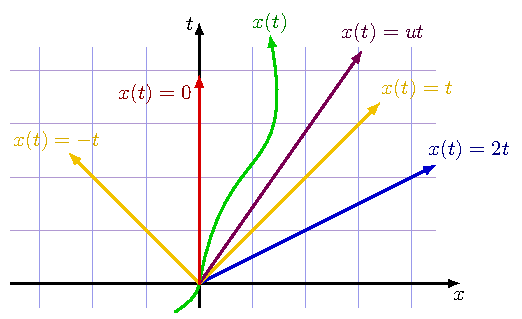
\includegraphics[width=.5\textwidth]{fig/chpt01/worldlines.pdf}
    \caption{\small 2 维时空图。以某惯性系为\textbf{绘图基准}是一种时空图的绘制习惯:将其坐标网格画成欧氏正交、时间轴未来方向朝上(空间轴右手排列)、尺度均匀的,这样迎合几何制,反向的光线也相互正交。}
\end{wrapfigure}

更普遍地,考察\textit{全体事件}规律排布的集合。比如,以某参考系为基准,可连续堆叠各时刻的同时事件集,即给空间补上时间轴就形成了\textbf{时空连续统}(spacetime continuum),简称\textbf{时空}。
故同时事件集又可形象地称为\textbf{同时面}(simultaneity surface)。
由于存在不同参考系选择,故建议直接默认存在一个 4 维\textbf{流形}(manifold)作为时空的理想模型。
流形就是点连续分布形成的集合,从而能建立坐标系\footnote{最初,我们仅用微积分和坐标系研究背景的\textbf{局部}(local)性质,建立了\textbf{微分几何}(differential geometry)。随着集合论和\textbf{拓扑学}发展,我们发现可将背景准确称为\textbf{拓扑空间}(topological space),其上提供了连续性定义。赋有坐标系的拓扑空间即流形,总规定系 $\{x\},\{x'\}$ 间的变换 $x'^\mu=x'^\mu(x)$ 可逆且光滑,这样可随意做微积分。
拓扑学提供了分析\textbf{整体}(global)性质的工具,便有了\textbf{现代微分几何}。}。
同时面只是截取时空的一系列切片。
实际上物理研究总要预设背景流形。比如,Newton 力学的研究背景是 $\R^3$ 空间;亦或更为抽象,如热力学会研究压强、温度的相图。
无论坐标系选取如何,描述任一事件的 4 个坐标依次记作 $x^0,x^1,x^2,x^3$,约定 $x^0$ 对应时间,正方向为\textbf{未来},反方向为\textbf{过去},其余坐标对应空间。比如选择 Descartes 系 $\{x,y,z\}$:
\eq{
x^0:=ct,\quad x^1:=x,\quad x^2:=y,\quad x^3:=z.
}
其中给时间乘上无歧义常数 $c$ 以使量纲一致。此后多采用几何制($c=G=1$),则 $x^0=t$,这样 $x^0,t$ 都可称\textbf{坐标时}。
时空中的曲线称\textbf{世界线}(worldline)。一族世界线构成\textbf{世界管}(worldtube)或\textbf{线汇}(congruence) $\mathscr C$。参考系 $\mathscr R$ 就是其每条世界线 $\gamma$ 都有观者对应的世界管。无交叉线汇 $\mathscr C$ 所占时空范围内每一点,都 $\exists! \alpha\in\mathscr C$ 对应。各观者按 $a^i$ 编号,且用固有时 $a^0$ 参数化,便建立了所谓\textbf{共动系}或\textbf{固有系} $\{a\}$。将实际对象从粒子改为流体质元,则观者即流线,进而对应于流体力学的 Lagrange 表述。凡示意时空及世界线的图就是\textbf{时空图}(spacetime diagram)。就一般的四维时空,固然画不出直观图像,但许多问题总能借助对称性,省略部分空间维度。

这些概念看起来都很显然,但事实远非如此:时空结构很可能极其怪异。
我们有野心将时空流形施以整个宇宙,但宇宙的拓扑形状迄今未知,也许在大尺度上无法用 $\R^4$ 覆盖;在 $10^{-15}$\,m 或 $10^{-25}$\,m 的小尺度上,不可能建立起足够刚性的参考系。目前我们认为这是因为微观量子性质,但也或许存在更深刻的物理。Wheeler 认为在 $10^{-35}$\,m 的亚核子尺度,量子引力的涨落极其剧烈,产生量子泡沫,戳破时空连续统。量子引力理论必须一致包含常数 $c,G,\hbar$,其中 $\hbar=h/2\pi$ 是约化 Planck 常数。简单分析可构造出具有长度量纲的\textbf{Planck 长度} $\sqrt{\hbar G/c^3}\approx 1.6\times10^{-35}$\,m,这意味着涨落的特征尺度在 Planck 长度的量级。
即便如此,人类仍只能间接地探测变态性质,即假设时空能用连续坐标描述。若基于这一假设成功描述了涨落,就有理由相信,至少日常生活中的时空结构良好,因为 Planck 长度确实太小。
对于复杂的拓扑,仍然希望邻域上能连续地标记坐标,用 $\R^4$ 去近似。这正是流形的定义。拓扑背景不提供物理量的计算能力。


默认光速不变导致的遗憾是:有限能量下,亚光速有质粒子不能加速至光速。目前未发现超光速的快子(tachyon),故我们更愿意承认亚光速粒子、光子在时间上的连续性,即确认某两事件属同一粒子。凡信息就需载体,故光速是信息传速上限。注意,存在粒子能依次经历的两事件才称有\textbf{因果联系},可见并非所有事件都能涉及因果。
相互作用是一种信息,物质总通过动量、能量、质量的变化反馈。
可见相互作用至多以光速影响邻域,此即\textbf{定域性}(locality)或\textbf{局域性}。
从而,我们总能适当忽略环境对所关心的系统的作用以建立\textbf{孤立系统}模型,即忽略环境与系统的动量、能量、质量交换。此乃物理研究之根基:
宇宙是无所不包的最大时空,但我们往往只关心某些局部区域,即宇宙子系统。
理解子系统必须且可以使用孤立系统,否则讨论任何客体时都须考虑整个宇宙的作用,结果一事无成。
经典力学无定域性。Newton 引力定律是典型的超距案例,任二事件可通过 Newton 引力涉及因果。这一定律现只作为近似。对不具备连续性的事件亦能定义速率,比如介质光速。谈论超光速现象时往往指这种含义,以因果为前提的速度自然默认亚光速。

场提供了定域性最自然的图像,迄今所有基本相互作⽤都归结于定域场。两相距较远的粒子的相互作⽤解释为:粒子(作为\textbf{源})与场接触作用,再由场接触作用于另一粒子。接触作用强度均涉及粒子的\textbf{荷}(charge)。实际上,由于粒子动量、能量变化,为保持总和守恒,须设想粒子将其传递给周遭弥漫着的某种媒介。
起初我们这样理解场论:设想一种\textbf{试验粒子}(test particle),忽略其体积、形变及自旋,最重要地是忽略其自场对外场之干扰,就能测量受力来研究外场。每单位荷的场力即\textbf{场强}(strength),通常无关于试验粒子,往往又能表为某个\textbf{势}(potential)之导数。
在量子场论中,粒子解释为量子场的激发态。质子、电子、夸克等 Fermi 子携带作用荷,Bose 子场提供作用媒介。比如,电子场影响电磁场,产生波包(光子)传递电磁作用,在低能情形表现为电磁力。故严格来说,电磁场不依附于某个带电体,将总场分解为由各源所产生的部分是一种经典分析方法。

\subsection{Lorentz 不变性}

如何对钟?
首先想到单程信号。人类总依靠观者和被观测物的信息交流来感知世界,比如能给予视觉图像的可见光,或天文观测。
无论可见光还是神经元生物电,其速率皆有限,传播过程花费时间,图像通常存在扭曲和滞后\footnote{对高速物体、强引力场现象的测算足以总结为一门课题,又同计算机图形学结合,称为\textbf{相对论视觉}。},
故不可能通过单程信号真正体会与周围的同时性。当然,这些信号依旧很快,以至于直到 Einstein 之前,人类都对同时性保有错觉。

\begin{figure}[ht]
    \centering
    \subfloat[\centering 静系对钟]{
    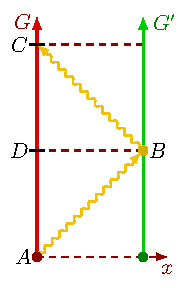
\includegraphics[height=.41\textwidth]{fig/chpt01/reflecting.pdf}
    }%
    \qquad
    \subfloat[\centering 动系对钟]{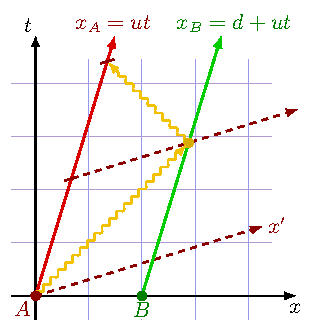
\includegraphics[height=.4\textwidth]{fig/chpt01/reflec2.pdf}
    }%
    \caption{\small 若以 $G$ 为绘图基准,只需使反射光与 $G$ 夹角呈 $45^\circ$ 即可使 $BD,AC$ 正交,结果如(a)。以该系为基准,研究一个运动惯性观者的对钟情况,结果如(b)。可见惯性系的坐标轴总关于 $45^\circ$ 斜线对称。}
    \label{fig:clock_syn}
\end{figure}

随后我们想到双程信号。
先讨论惯性参考系。
规定\textbf{惯性观者}走匀速直线。
无论技术发展如何,双程光速的测量原理至今仍和\textbf{Fizeau 程序}一致:从坐标原点发射球面光波,然后由放置在某处(尽量邻近)距离已知的镜子反射,随后记录光回到原点的时间,这样可计算光速。按现在的约定,不需要再测量光速,故以上步骤更倾向于测距。
任取某条惯性观者线 $G$,规定为坐标原点。设相对静止的另一惯性观者 $G'$;实验上若任意时刻测距均相同,就认为二者相对静止。二者可同属一个惯性参考系。
$G$ 在某时刻发出光(事件 $A$),到达 $G'$ 反射(事件 $B$),最后 $G$ 在某时刻接受该光(事件 $C$)。取 $A,C$ 的中间事件 $D$;实验上由标准钟测量。只需约定 $B,D$ 同时。
按此规定,惯性参考系的共动系称为\textbf{惯性坐标系}或\textbf{Lorentz 系}。不必认真区分时可笼统称为\textbf{惯性系}(inertial frame)。
总之,单程光速是约定的,不可实验测量(除非找到非光对钟法);我们可以测量的是双程光速,且用平均逼近瞬时。
且注意,并非所有参考系都能办到对钟。

时空正交性通常定义为:对钟后的同时面与各观者线正交\footnote{理论上的几何概念只能代数地定义,如勾股定理。实际用物理定律来约定一类基准,各类规则形状的日常用品就是这样生产的。比如,默认光走直线、Lorentz 力确定空间正交性、宇称不守恒确定右手性。}。虽然时空图中动系坐标轴不是欧氏正交,但被约定为时空上的正交。

\begin{figure}[t]
    \centering
    \subfloat[\centering $A,B$ 在 $S$ 中同时]{
    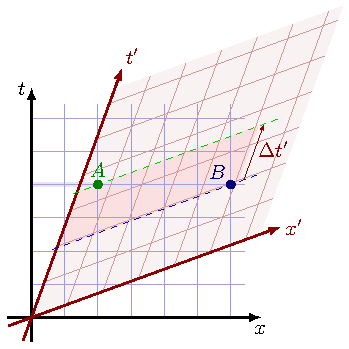
\includegraphics[width=.35\textwidth]{fig/chpt01/SIMULTANEITY.pdf}
    }%
    \quad
    \subfloat[\centering $A,B$ 在 $S'$ 中同时]{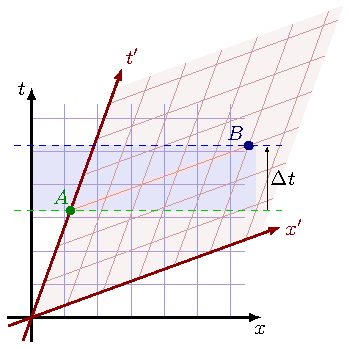
\includegraphics[width=.35\textwidth]{fig/chpt01/SIMU2.pdf}
    }
    \caption{\small 作某事件的同时面可投影得其坐标时。设静系 $S$ 和动系 $S'$。某事件的 $t$ 坐标可做 $S$系同时面截得,而 $t'$ 坐标可做$S'$系同时面截得。
    两个超新星的爆发事件在某系同时,但一般在另一系不同时。无法区别出特定的同时面,此即\textbf{同时的相对性}。}
    \label{fig:simurela}
\end{figure}

考虑任意惯性运动对象 $\gamma$ 于事件 $\gamma(\tau_1),\gamma(\tau_2)$ 经历的(elapsed along)固有时间 $\Delta\tau=\tau_2-\tau_1$。
惯性观者 $G$ 有办法直接测算这一时间吗?假设在 $G$ 系 $\{t,x,y,z\}$ 看来,$\Delta t$ 内 $\gamma$ 走过 $\Delta x,\Delta y,\Delta z$。Descartes 系的勾股定理为$\Delta\ell^2=\delta_{ij}\Delta x^i\Delta x^j$,其中 $(\delta_{ij})$ 为单位阵并对指标使用求和约定。$\delta_{ij}$ 称为\textbf{Kronecker 符号}。速率可写作 $u=\Delta\ell/\Delta t$。
总可设置与 $\gamma$ 相距 $L$、相对静止的镜子使光从 $\gamma(\tau_1)$ 发出并反射回 $\gamma(\tau_2)$,且镜面平行于运动方向。
由 $\gamma$ 系知 $2L=\Delta\tau$。
关键在于 $G$ 系中,镜面间距仍为 $L$,因为间距与运动方向垂直\footnote{测量长度即用量尺同时观察两端,涉及同时性。对任意沿垂线方向运动的尺 $A$,总可设置静止的尺 $B$ 使二者中垂线重合且静长相同。在 $B$ 看来,整个系统关于中垂线对称,故 $A$ 两端必同时到达 $B$ 所在直线,从而判断 $\sgn$($A$ 动长 - $B$ 静长),$\sgn$ 表示取符。这也等于 $\sgn$($A$ 静长 - $B$ 动长),因为在 $A$ 看来也有中垂线对称性,故这两个相遇事件在 $A$ 系也同时。但 $A$ 静长 = $B$ 静长,因此两个观者所处的情形是一致的,只是有反转或 $180^\circ$ 的对称。由相对性原理知 $\sgn$($A$ 动长 - $B$ 静长) = $\sgn$($B$ 动长 - $A$ 静长) = -$\sgn$($A$ 动长 - $B$ 静长),故 $A$ 动长 = $B$ 静长 = $A$ 静长。}。
由光速不变知 $2\sqrt{L^2+\Delta\ell^2/4}=\Delta t$,则 $\Delta\tau^2=\Delta t^2-\Delta\ell^2$,或者 $\Delta t=\gamma\Delta\tau$,其中 $\gamma:=1/\sqrt{1-u^2}\geqslant 1$ 是\textbf{Lorentz 因子}。可见 $\Delta t\geqslant\Delta\tau$,在观者看来,运动的时钟走时慢,这种现象称为\textbf{钟慢效应}或\textbf{时间膨胀}。这种效应是对称的,每个观者都认为其它的相对运动的时钟走时慢。
比如,宇宙射线含有介子,但其寿命非常短,即使以光速运动,穿透大气层所需时间也通常是寿命的几十倍。按理来说它不可能到达地面,但钟慢效应使其保持年轻,寿命“延长”,故仍可到达。

根据相对性原理,对任二惯性系 $\{x\},\{x'\}$ 必有两事件\textbf{间隔}(平方)$\Delta s^2:={\eta}_{\mu\nu}\Delta x^\mu\Delta x^\nu$ 的不变性,其中 $({\eta}_{\mu\nu}):=\diag(-1,1,1,1)$,即
\[-\Delta t^2+\Delta x^2+\Delta y^2+\Delta z^2=-\Delta t'^2+\Delta x'^2+\Delta y'^2+\Delta z'^2.\]
而 Newton 理论则分开定义绝对时间长度和空间长度。
$(\eta_{\mu\nu})$ 作为广义的单位阵,易证 $(\eta_{\mu\nu})=(\eta^{\mu\nu})$。
定义\textbf{号差}(signature)为 $(\eta_{\mu\nu})$ 的迹,本书一般选择 $+2$,称为\textbf{东海岸}习惯\footnote{量子场论教材常选择 $(\eta_{\mu\nu})=\diag(1,-1,-1,-1)$,号差为 $-2$ 即\textbf{西海岸}习惯。更有甚者选择将时间分量排在最后作为第 4 分量,这样有 $\diag(1,1,1,-1)$ 但并不影响号差。也有一种可能有哲学区别的习惯,称\textbf{Wick 技巧}:令 $x^0=\i ct$ 则线元还原回勾股定理 $\d s^2= \delta_{\mu\nu}\d x^\mu\d x^\nu$,伪转动变换的确变为 $x$-$\i ct$ 平面的旋转变换。除讨论某些理论复结构方面的问题外不使用这种做法。}。
该号差下,按 $\Delta s^2$ 为正、负或零,可分别称为\textbf{类空}(spacelike)、\textbf{类时}(timelike)或\textbf{类光}(lightlike)间隔。间隔不变性对类时间隔成立($\Delta\tau^2=-\Delta s^2$)。对类光间隔,注意光速不变与 $\Delta s^2=0$ 等价,仍成立。考察类空间隔。再次利用光测距,设置相对静止的镜子惯性运动,表示待测间隔。入射光的固有用时 $\Delta s$,出射光亦是 $\Delta s$。
外部观者看来,入射光用时 $\frac{L}{1-u}=\gamma\Delta s+\Delta t$,出射光用时 $\frac{L}{1+u}=\gamma\Delta s-\Delta t$。总共 $2\gamma\Delta s=\frac{L}{1-u}+\frac{L}{1+u}=2\gamma^2L$,则 $L=\Delta s/\gamma\leqslant\Delta s$。即运动方向上缩短 $1/\gamma$ 倍。这种现象称为\textbf{尺缩效应}或\textbf{长度收缩}。
蟹状星云和半人马星座 $\alpha$ 星之间的距离是相对的,不必诧异。
进而 $\Delta t=\gamma u\Delta s$。入射光总共走过 $\frac{L}{1-u}=\Delta\ell+\gamma u\Delta s$,则 $\Delta\ell = \gamma\Delta s$。故 $\Delta s^2=-\Delta t^2+\Delta\ell^2$,成立。

    \begin{figure}[t]
        \centering
        \subfloat[\centering 在 $S$ 中静止]{
        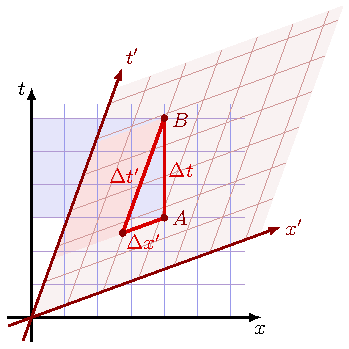
\includegraphics[width=.35\textwidth]{fig/chpt01/TIME DILATION S.pdf}
        }%
        \qquad
        \subfloat[\centering 在 $S'$ 中静止]{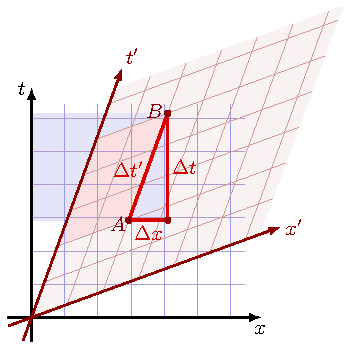
\includegraphics[width=.35\textwidth]{fig/chpt01/TIME DILATION S'.pdf}
        }
        \caption{钟慢效应}
    \end{figure}

考虑无穷小的事件间隔或\textbf{时空线元}
\eq{
\d s^2={\eta}_{\mu\nu}\d x^\mu\d x^\nu=-\d t^2+\d x^2+\d y^2+\d z^2.
}
设任意(分段光滑的)观者线 $C(\sigma)$,$\sigma$ 是任取参数,可有 $\gamma=\dv*{t}{\tau}$。考察它于事件 $C(\sigma_1),C(\sigma_2)$ 的固有时间 $\Delta\tau$。设置其固有坐标系 $\{x'\}$($x'^0=\tau$),$C$ 上事件总满足 $x'^i=0$,则 $\d\tau^2=-\d s^2$。它在惯性系 $\{x\}$ 下的参数式记 $x^\mu(\sigma)$,则
\eq{
\Delta\tau=\int_C \sqrt{-\eta_{\mu\nu}\d x^\mu\d x^\nu}=\int_{\sigma_1}^{\sigma_2}\sqrt{-\eta_{\mu\nu}\dv{x^\mu}{\sigma}\dv{x^\nu}{\sigma}}\d\sigma=\int_{\sigma_1}^{\sigma_2}\sqrt{-\eta_{\mu\nu}T^\mu T^\nu}\d\sigma,}
$T^\mu:=\dv*{x^\mu}{\sigma}$ 为关于 $\sigma$ 的\textbf{切矢}(tangent vector)在该系的分量,$\eta_{\mu\nu}T^\mu T^\nu$ 即模方。
切矢按模方符号(进而相应曲线)可类似分为三类。
\begin{figure}[t]
    \centering
    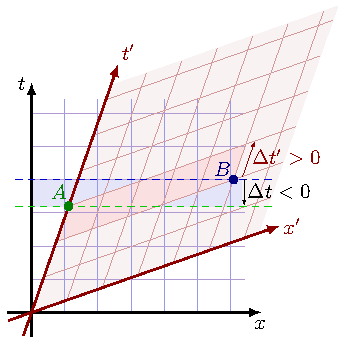
\includegraphics[width=.35\textwidth]{fig/chpt01/order.pdf}
    \caption{\small 若间隔类光或类时,则(由 $\Lambda^0{}_0>0$ 联系)各惯性系将一致认同两个事件的先后顺序。但对于类空间隔,其事件的坐标时差距可以在不同惯性系下取任意实数。不同观者对其先后次序各抒己见。
    类空间隔的事件没有因果联系。}
    \label{fig:spacelike}
\end{figure}
类时或类光线统称\textbf{因果线}(causal curve),能用因果线连接的事件正是具有因果联系的事件。在 $\R^4$ 中这等价于用非类空间隔连接。
类光矢量亦称\textbf{零模}(null)矢量,构成的集合 $C_N$ 称\textbf{光锥}(light cone)。
$\Delta\tau$ 即观者线的线长,故 $\tau$ 又称\textbf{线长参数}。$\lambda=a\tau+b$ 统称\textbf{仿射参数}(affine parameter)。
光对其世界线上的事件标记为一致坐标时,即对光而言不能定义固有时。光不能充当观者。描述光线可用坐标时 $t$ 参数化。

设 $V^\mu$ 类时,$W^\nu$ 是非零类时或类光矢量,则由三维 Cauchy 不等式知 $V^\mu W_\mu<0\eqto V^{0} W^{0}>0$,即 $V^\mu,W^\nu$ 具有相同的\textbf{时间指向}。
因此可在光锥及其内部定义等价关系。约定某一惯性系后,规定 $V^0>0$ 是\textbf{指向未来}(future directed)矢量,那 $V^0<0$ 是\textbf{指向过去}(past directed)矢量。光锥被分为了\textbf{未来光锥}和\textbf{过去光锥}。讨论时间的反演时可以考虑指向过去的惯性系。类空矢量无未来或过去之分。

\begin{figure}[t]
    \centering
    \subfloat[\centering 3 维时空的光锥]{
     \begin{tikzpicture}[scale=1.5]
    \draw (-1,-1)--(1,1);
    \draw (-1,1)--(1,-1) node[right]{$\scriptstyle C_N$};
    \draw[->] (0,0)--(0.8,0.8) node[below right]{\scriptsize 类光矢量};
    \draw[->] (0,0)--(-0.9,-0.3) node[above left]{\scriptsize 类空矢量};
    \draw[dashed] (0,0)--(-0.175,0.175/0.2);
    \draw[->] (-0.175,0.175/0.2)--(-0.25,0.25/0.2) node[above left]{\scriptsize 类时矢量};
    \draw (0,1)  ellipse [x radius=1, y radius=0.13];
    \draw[dashed] (1,-1) arc [start angle=0, end angle=180, x radius=1, y radius=0.13];
    \draw (1,-1) arc [start angle=0, end angle=-180, x radius=1, y radius=0.13];
    \end{tikzpicture}
    }%
    \quad
    \subfloat[\centering 因果结构]{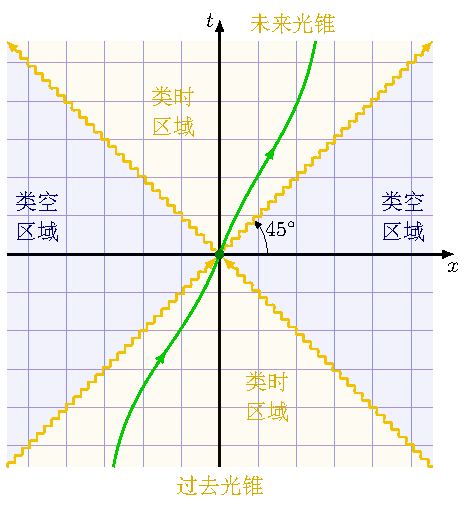
\includegraphics[width=.3\textwidth]{fig/chpt01/structure cone.pdf}
    }
    \caption{光锥}
\end{figure}

惯性系 $\{x\},\{x'\}$ 间满足
\eq{\eta_{\alpha\beta}\d x'^\alpha\d x'^\beta=\eta_{\gamma\sigma}\d x^\gamma\d x^\sigma\iff \eta_{\alpha\beta}\pdv{x'^\alpha}{x^\gamma}\pdv{x'^\beta}{x^\sigma}=\eta_{\gamma\sigma},}
由 \eqref{eq:chris} 式可快速证明变换的仿射性:
\eq{\label{Lorentz} 
\pdv{x'^\alpha}{x^{\gamma}}{x^\epsilon}=0\iff  x'^\mu=x_0^\mu+ \Lambda^{\mu}{}_{\nu}x^\nu,\quad \text{$\Lambda^{\mu}{}_{\nu}$ 满足 $\eta_{\mu\nu}\Lambda^{\mu}{}_{\sigma}{\Lambda^{\nu}}_{\lambda}={\eta}_{\sigma\lambda}$}.
}
满足上式的变换称\textbf{Poincaré 变换}。
置 $S,S'$ 的时空原点重合,则 $x^\mu_0=0$,变换仅线性。设空间轴初态重合,但 $S'$ 相对于 $S$ 沿共同 $x,x'$ 轴匀速运动,则 $y,z$ 坐标一致。设正方向速率 $u$,则 $x=ut$ 对应 $x'=0$。    
进而得到(或直接利用钟慢、尺缩)\textbf{二维 boost 变换}:
\eq{
     t'=\gamma( t-u x),\quad x'=\gamma( x-u t).
}
普通教材称之 Lorentz 变换。Einstein 最初用同时性对钟定义、仿射性假设得到上式,而线元后来才由 Minkowski(参见 \cite{PrincipleR})提出。
由此发展出来的理论由 Lorentz 命名为\textbf{相对性理论}(the theory of relativity),简称\textbf{相对论}。当下主流称呼是\textbf{狭义相对论}(special relativity)。boost 变换仅为特例,一般情形的推导见 \ref{sec:PoincareLorentz} 节。
因为上式在低速极限下退回 Galileo 变换 $t'=t,x'=x-ut$,从而兼容经典力学。
“boost”取时间轴上的推动之意,但由图 \ref{fig:boost} 可知,一个较好称呼是\textbf{伪转动}(pseudo rotation)。

\begin{figure}[p]
    \centering
    \subfloat[\centering 空间转动变换]{
    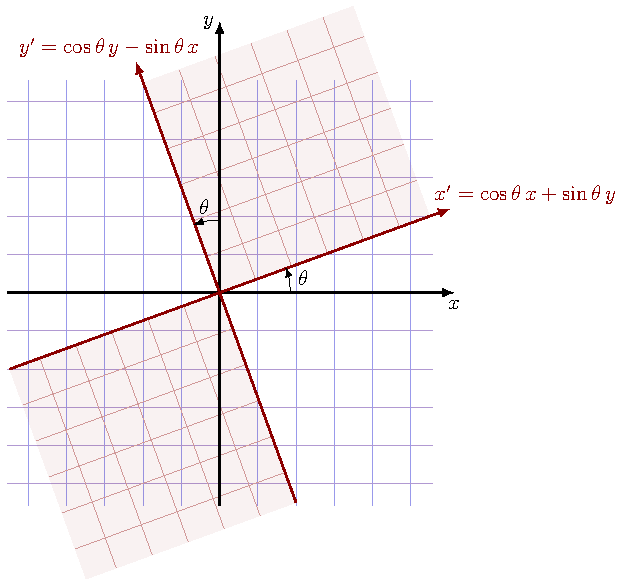
\includegraphics[width=.45\textwidth]{fig/chpt01/ROTATION.pdf}
    }%
    \subfloat[\centering 时空伪转动变换]{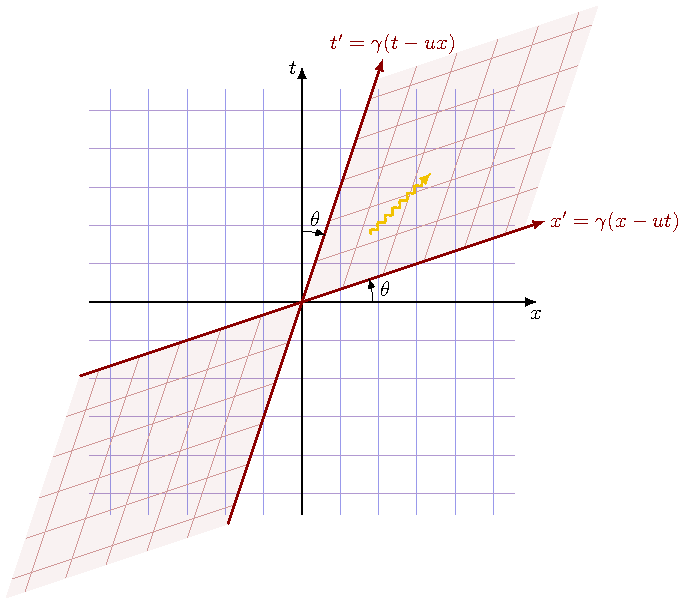
\includegraphics[width=.49\textwidth]{fig/chpt01/boost.pdf}
    }

    \subfloat[\centering 负方向伪转动]{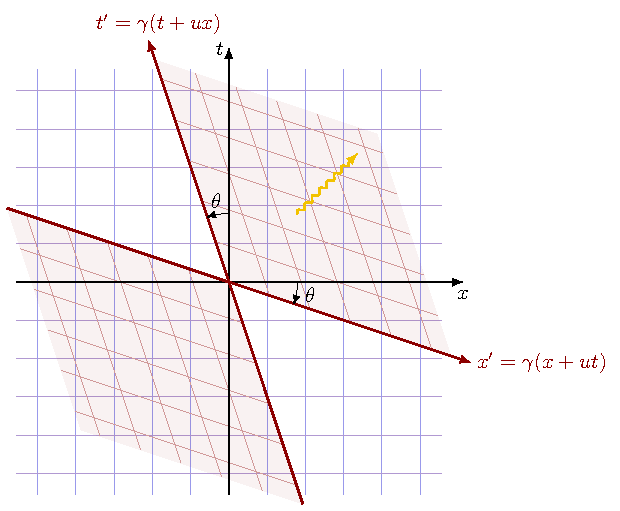
\includegraphics[width=.44\textwidth]{fig/chpt01/INVERSE BOOST.pdf}
    }
    \subfloat[\centering Galileo 变换]{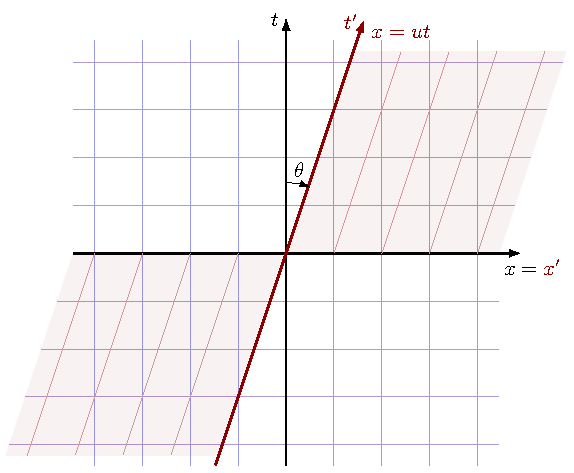
\includegraphics[width=.42\textwidth]{fig/chpt01/GALILEAN.pdf}
    }
    \caption{\small
    $x'$ 轴直线 $t'=0$ 即 $t=u x$,同理 $t'$ 轴即 $t=(1 / u) x$。速率 $u$ 代表动系时间轴斜率。以转动变换类比之,相应的三角函数应替换为双曲函数。$\theta:=\operatorname{artanh}u$不是绘图意义的倾角,称为\textbf{快度}。这样 $\cosh\theta=\gamma,  \sinh\theta=\gamma u$,变换为 $t'= t\cosh\theta - x\sinh\theta, x'= x\cosh\theta -t \sinh\theta$。
    如图,光速相对于日常情形较大,因此图上光线应“下压”,则空间轴转动不明显,退回 Galileo 变换,大家共用绝对时间。快度概念比速度更简洁。比如,设 $u_1=\tanh\theta_{1}$ 是 $B$ 相对于 $A$ 的速度,而 $u_2=\tanh\theta_{2}$ 是 $C$ 相对于 $B$ 的速度,可证 $C$ 相对于 $A$ 的速度是 $u={(u_{1}+u_{2})}/{(1+u_{1} u_{2})}=\tanh(\theta_1+\theta_{2})$,此即速度叠加公式。
    }\label{fig:boost}
\end{figure}

物理学用矩阵书写物理量,如标量、矢量;Cauchy 研究弹性力学时还意识到,一点处质元与质元的作用力不能只由一个数组描述,需用多维矩阵,称之为\textbf{张量}(tensor)。
物理量总与其分量联系,因为观者只能利用仪器的坐标系测量分量,提取实验数据。
关键就在于坐标变换下物理量的分量如何变。
分量及其方程的数学形式在某类坐标变换下不变,称为\textbf{协变性}(covariance)。狭义相对论具有 Lorentz 系间变换下的\textbf{Lorentz 协变性}。
现在就可更严格地阐述狭义相对论的原理:\textit{物理方程具有 Lorentz 协变性,且与物质状态无关的标量常数保持同样的值},如 $c=1,\pi/2$ 和 $\hbar$。合称\textbf{Lorentz 不变性}(invariance)。
例如,经典电动力学虽然能将光解释为无源电磁波,但 Maxwell 方程的 Lorentz 协变性只涉及其数学形式,将协变性提升为不变性才能给出光速不变。

原则上,当然存在满足光速不变、相对性原理,但非 Lorentz 不变的理论,因为前文推导实际上默认了通常的额外条件,比如光走直线、不存在其它不变常数;甚至将来可能存在实验证否光速不变或相对性原理。但相对论以及在此基础上发展的量子场论的许多结果,都在极高精度上获得验证。我们目前有充分理由认可 Lorentz 不变性,直至存在实验证否。

\newpage
\begin{figure}[!h]
    \centering
        \subfloat[\centering 双曲线校准]{
        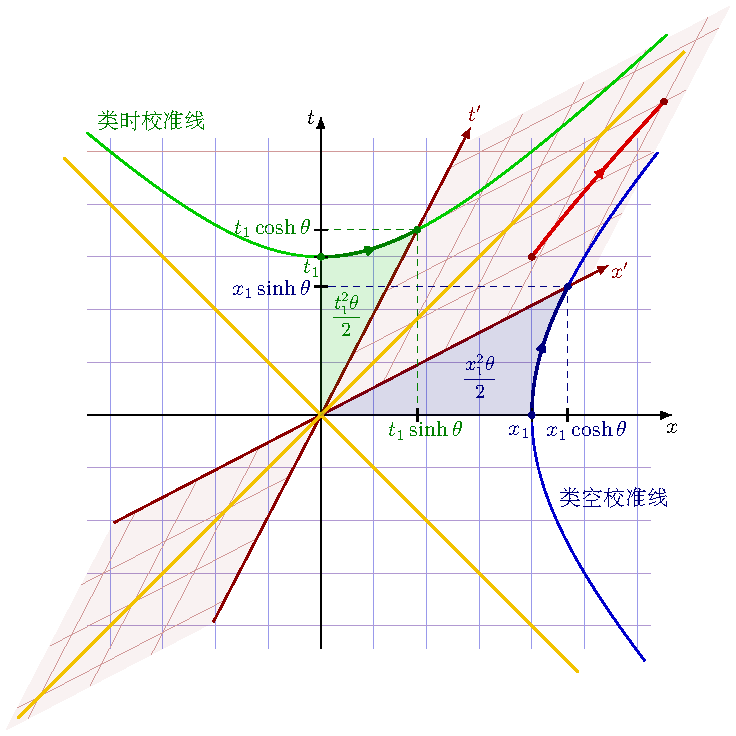
\includegraphics[height=.45\textwidth]{fig/chpt01/HYPERBOLOIDS.pdf}
        }
        \subfloat[\centering 钟慢效应]{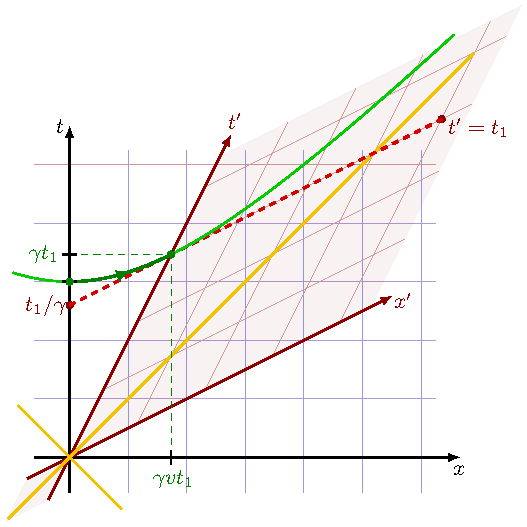
\includegraphics[height=.45\textwidth]{fig/chpt01/INVARIANT HYPERBOLOIDS.pdf}
        }
    \caption{\small 比较间隔的方法是用双曲线校准。令双曲线 $x^2-t^2=x_1^2$,其与 $x$ 轴交于 $\left(t,x\right)=(0,x_1)$。双曲线上的点 $(t,x)=(x_1\sinh\theta, x_1\cosh\theta)$ 与原点连线是类空间隔且恒定,可用来比较类空间隔,故称\textbf{类空校准线}。从 $(0,x_1)$ 至 $(t,x)$ 扫过角度 $\theta$,易得扫过面积为 $x_1^2\theta/2$,可类比欧氏几何的圆。同理推知\textbf{类时校准线}的结论。
    例如,两个观者都看到 $S$ 系原点上的时钟读数“0”,但直线 $t'=t_1$ 与该时钟世界线($t$ 轴)在 $\left(t,x\right)=(t_1,0)$ 下方的 $(t_1/\gamma,0)$ 相交。故$S'$ 系的钟根据同时面 $t'=t_1,t'=0$ 认为 $S$ 的钟慢。}
\end{figure}
    \begin{figure}[!h]
        \centering
        \subfloat[\centering 在 $S'$ 中静止]{
        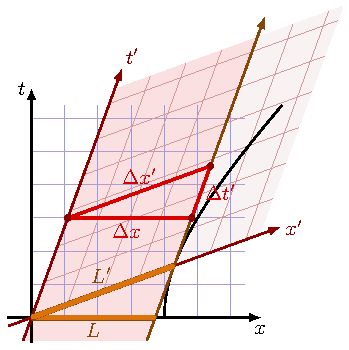
\includegraphics[height=.45\textwidth]{fig/chpt01/INVARIANT 2.pdf}
        }
        \qquad
        \subfloat[\centering 在 $S$ 中静止]{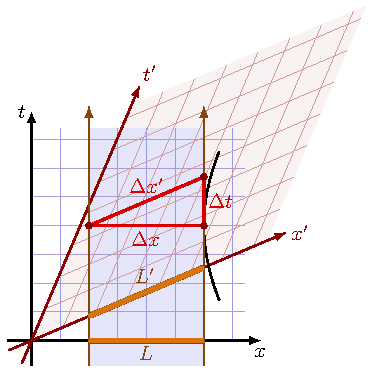
\includegraphics[height=.45\textwidth]{fig/chpt01/INVARIANT 1.pdf}
        }
        \caption{\small 尺缩效应}
    \end{figure}
\newpage
    
\begin{wrapfigure}{l}{.45\textwidth}
    \centering
    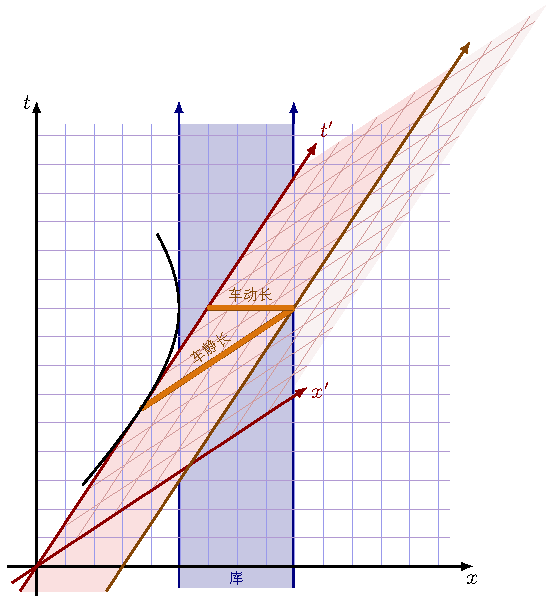
\includegraphics[width=.45\textwidth]{fig/chpt01/ladder.pdf}
    \caption{汽车匀速进库}
\end{wrapfigure}
    
    尺缩效应还导致\textbf{车库佯谬}\footnote{Ladder paradox,由 Rindler 提出,最初借梯子和谷仓(barn)举例,还可用火车和隧道。}。
    设汽车与车库静长相等。汽车朝库匀速前进,司机认为动库变短、不能放下,司库认为动车收缩、放下有余。二者矛盾吗?不妨设车库无后墙(类似于隧道洞口),画图时借用校准曲线以保证车和库有相等静长。由图易见,以司库所在惯性系的同时面衡量,车短于库;以司机所在惯性系的同时面衡量,车长于库。两人观点都对,因为同时性的相对性导致结论的相对性。“\textit{到底}放下还是放不下?”这种问题没有意义,正如在尺缩问题中“到底哪把尺子较长”亦无意义。我们若真要“比较”,能让各位意见一致的做法只能是都放入静系中去。
    从因果角度来理解将更便于在脑海里建立物理图像。“车尾接触入口”“车头接触出口”两个事件没有因果联系,故二人观点都对。我们在脑海中,不假思索地以为有因果联系,这个错觉来源于火车的车身。但在相对论中没有严格的刚体,只能将车身各质元的恒定高速运动理解为独自的、互相影响很小的。当然,现实生活中没有这么长且如此高速的火车,相互作用能在车头车尾间迅速传递,的确具有因果联系。
    当车库有坚硬后墙时,车头固然撞墙停止。但撞墙信息以相互作用纵波传至车身各部分皆需时间,只当车尾获悉后整个车身才能停住,因而汽车将缩至比司库期初所测
    
    \begin{wrapfigure}{r}{.35\textwidth}
        \centering
        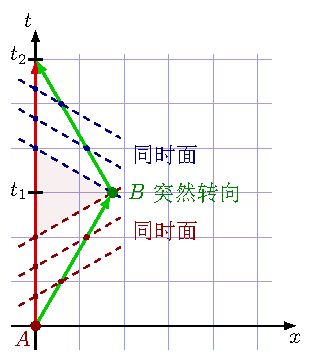
\includegraphics[width=.35\textwidth]{fig/chpt01/TWIN PARADOX.pdf}
        \caption{孪生佯谬}
        \label{fig:twin}
    \end{wrapfigure}

    \noindent 长度更短的程度。这时的确在谁看来都装得下。设材料性质理想,使信息传递为光速且质点获悉信号后立即停止,读者不妨在图上补出撞车后的时空图。

    最后,著名的\textbf{孪生佯谬}(twin paradox)就是说,设一对双胞胎从某时空点分离,并回合于另一时空点,则惯性运动者将年长于非惯性运动者。
    前文已直接证明了这一点。图 \ref{fig:twin} 给出了三角情形,也可理解为,折线的同时面在 $B$ 处发生突变,因此惯性观者多出了图中阴影部分的时间差。
    结论是不能交换的,因为不能将相对性原理滥用于非惯性系和惯性系间;而实际情形中,两人非质点,因此走惯性运动较为舒适,而走非惯性运动将感受到巨大的加速度,使相对论现象足够明显的物理量达光速级。


\subsection{惯性系存在性}

前文对惯性系存在性的考虑,仍然承袭 Newton 体系的思维,即认为存在一个绝对静止系,则相对其匀速的物体可作为惯性系,而具有加速度的物体不能充当惯性系。然而,并无任何先验原理帮助我们确定绝对静止系在哪。
实际上,物质间皆存在引力,且可在长程上传递,这称为引力的\textbf{万有性},而理想惯性系必须远离所有物质以孤立,因此严格来说不存在。但实验上 Newton 定律一定程度适用于地面系,可见惯性系仍是有用概念。问题出在哪里?

物质在仅受引力作用时有\textbf{Galileo 性}:任意试验质点在同一时空点所受加速度相同(由任意坐标系测量),与内部结构及组成无关。Newton 对 Galileo 性的解释如下。$\bm f=m_I\ddot{\bm x}$ 定义的质量 $m_I$ 是\textbf{惯性质量}。Mach 提出了一种测量性定义:承认动量守恒并规定好某一物体的质量数值,使二者产生相互作用(如碰撞),根据加速度比值便可测得另一物体的质量。而 $\bm f=m_G\bm g $ 定义的质量 $m_G$ 是\textbf{引力质量}或\textbf{引力荷}。联立有 $\ddot{\bm x}=(m_G/m_I)\bm g $,说明 Galileo 性即指比例 $m_G/m_I$ 与物质本身无关,重新定义 $G,m_G$ 还可使此二概念不再区分:$m_I=m_G\Rightarrow\bm g =\ddot{\bm x}$。
设 $A,B$ 共同自由落体,二者相对加速度近似为零。关键在于,\textit{总能以一者为研究对象,另一者抽象为背景坐标系}。比如,$B$ 可以是一部足够小、无自转的封闭电梯,而 $A$ 是乘客,则 $A$ 将感到失重。Newton 理论指出 $B$ 系中出现惯性力,但它与引力局域抵消,$B$ 系中做任何局域的力学实验结果都与惯性系等效,尤其在抛弃绝对系概念后,我们无法分辨。

对任意自由落体质点而言,总存在局域坐标系,使质点相对于该系的动力学,像是在理想惯性系中一样。这种坐标系称为相应质点的\textbf{局域惯性系}。参考系的惯性性在局域上不可物理观测,惯性系可以且只能局域建立。任何我们所规定的惯性系,其实均是局域惯性系。Newton 的绝对运动不是相对于绝对系的运动,而是相对于局域惯性系的运动。
Einstein 于 1907 年察觉到这一等效性\footnote{顺便提一句,Newton 是知道这件事的:“\textit{无论诸物体彼此间以何种方式运动,若它们被沿着平行线的相等加速力所推动,则它们都将继续彼此间的运动,遵循的方式就如同没有那些力作用一样}。”——《原理》\cite{Principia} 推论 VI “运动定律”。可用这个推论来计算太阳系中月球的复杂运动。在地球系下,惯性力和太阳引力在良好近似下相互抵消,那么月球就遵循一个 Kepler 轨道。}。
尽管 Galileo 性是谈及质点的,但他坚信任何物质都应如此,他称之为\textbf{等效原理}(equivalence principle)。这里要包括电磁、量子等任何实验:容易想象,在落体电梯里打开手电筒,光相对电梯按一定频率走直线,而在地球上看光线只能弯曲且频率变化,便能预言光的偏折、红移。

现在再研究可多大程度上建立局域惯性系。对于两相距足够远的时空点,引力加速度一般不同。一水球各部分受力不均,从而出现形变。这就是\textbf{潮汐效应}。邻近质元间相对力也称\textbf{潮汐力}(tidal force),相对加速度称\textbf{潮汐加速度}。可见,理想的局域惯性系只建立在自由落体质点的世界线上。当然,只要在设备精度内未观测到潮汐,就可认为是实验意义的局域惯性系。若物质集团的尺度较大,密度较稀疏,则外部引力较弱,潮汐现象不明显,因此能近似为局域惯性系的时空区域很大。比如,地球、太阳系、银河系能作为局域惯性系的范围应依次增大。现在,理想惯性系只视作局域惯性系在无引力时延伸的极限。综上,实验意义的局域惯性系的范围由外部引力强弱决定。

\subsection{广义协变性}

等效原理指出惯性系与非惯性系局域难以区分,因而最好是认同任意参考系,即一种广义相对性原理。更进一步地,我们本就默认物理对象、规律不受坐标系影响,即\textbf{坐标冗余性},因而不仅考虑与参考系有关的那类坐标系,任意坐标系均可接受,即直接寻求对任意坐标变换的\textbf{广义协变性}。
由前文知曲线线长可由切矢的积分给出。
广义协变性要求同一切矢在任意坐标系下皆表以 $T^\mu=\d x^\mu/\d\sigma$ 形式,则根据全微分知:
\eq{
    T'^\mu= \pdv{x'^\mu}{x^\nu}T^\nu.
}
称这种变换为\textbf{逆变的}(contravariant),按这种方式变换的矢量称为\textbf{逆变矢量}(contravector)或切矢,故上指标又称\textbf{逆变指标}。一点处全体逆变矢量构成该点\textbf{切空间}(tangent space)。实际上,物理学很多矢量都与相切有关,因而是逆变矢量。可以存在变换与之互逆的矢量:
\eq{\omega'_i=\pdv{x^j}{x'^i}  \omega_j,}
则称\textbf{协变矢量}(covector)或\textbf{余切矢}(cotangent vector),简称\textbf{余矢}。下指标称\textbf{协变指标}。这一称呼与“协变性”有区别,没有物理方程“逆变性”的说法。

数学上给定 $\d s^2=g_{\mu\nu}\d x^\mu\d x^\nu$ 后用积分定义线长、矢量模,借圆弧和三角函数定义角,最后按投影定义切矢的内积(inner product),等价于 $g_{\mu\nu}V^\mu W^\nu$。可用该式定义内积,反之给出线长和夹角,此即线性代数教材的逻辑。$g_{\mu\nu}$ 乃人为给定,称为\textbf{度规}(metric)。据此定义有 $g_{\mu\nu}=g_{\nu\mu}$。取 Descartes 系,代入勾股定理 $\d\l^2=\delta_{ij}\d x^i\d x^j$ 就得欧氏几何,$\delta_{ij}$ 称\textbf{欧氏度规}。
欧氏几何现降级为一种选择,而非保守派所认为的绝对真理。比如 ${\eta}_{\mu\nu}$ 就是\textbf{闵氏度规};还可有双曲几何 $\d\l^2=(\d x^2+\d y^2)/(1-x^2-y^2)$,当接近 $x^2+y^2<1$ 边缘时,该线元相较于欧氏线元会越来越大,但它除平面几何第五公理外符合其余公理。公理的特征是可替代性,故这说明第五公理不能由其余公理推出,而只能作为欧氏几何的约束。\textbf{Gauss 假设}希望存在坐标系使线元表为勾股定理,进而在广义协变性要求下保持二次型:
\eq{
    g_{\mu\nu}\d x^\mu\d x^\nu=g'_{\gamma\sigma}\d x'^\gamma\d x'^\sigma\iff g'_{\gamma\sigma}= g_{\mu\nu}\pdv{x^\mu}{x'^\gamma}\pdv{x^\nu}{x'^\sigma}.
}
主流几何理论总研究二次型,不研究 $\d\l=(|\d x|^3+|\d y|^3)^{1/3}$ 等。上式是合同变换,$g_{\mu\nu}$ 保持可逆,故总可定义 $(g^{\mu\nu}):=(g_{\mu\nu})^{-1}$,即满足 $g^{\mu \lambda} g_{\lambda\nu}=g_{\nu\lambda}g^{\lambda\mu}=\delta^\mu_\nu$,其中 $\delta^\mu_\nu$ 也是 Kronecker 符号。称 $g^{\mu\nu}$ 为\textbf{度规逆}。
规定 $T_\mu$ 相应的\textbf{对偶矢量}(dual vector)为 $T_\mu:=g_{\mu\nu}T^\nu$,内积就可紧凑写作 $V^\mu W_\mu=V_\mu W^\mu$。它为协变矢量一例。也可对偶回去:$T^\mu=g^{\mu\nu}T_\nu$。

推而广之的概念称为\textbf{广义协变张量},本书简称张量。当然,称 $T^{\cdots}{}_{\cdots}$ 是张量,准确是想称分量等价类 $[T^{\cdots}{}_{\cdots}]=\{T^{\cdots}{}_{\cdots},T'^{\cdots}{}_{\cdots},\cdots\}$ 是张量。
$(k,l)$\textbf{型张量}简称 $(k,l)$-\textbf{张量},应满足如下\textbf{张量变换律}:
\eq{
    T'^{\mu_1\cdots\mu_k}{}_{\nu_1\cdots\nu_l}=T^{\rho_1\cdots\rho_k}{}_{\sigma_1\cdots\sigma_l}\pdv{x'^{\mu_1}}{x^{\rho_1}}\cdots\pdv{x'^{\mu_k}}{x^{\rho_k}}\pdv{x^{\sigma_1}}{x'^{\nu_1}}\cdots\pdv{x^{\sigma_l}}{x'^{\nu_l}},
}
可记忆为是满足指标平衡的 Jacobi 矩阵元乘积,这样就可快速写出公式。
常习惯于先将上指标写完,再错开地写下指标。
只要求 Lorentz 协变性 $\pdv*{x'^\mu}{x^\nu}=\Lambda^\mu{}_\nu$ 则称\textbf{Lorentz 张量}。张量一定是 Lorentz 张量,反之不然。
$(k+l)$ 叫作张量的\textbf{阶}(rank)。$(0,0)$-张量就是不变标量。$(n,0),(0,n)$ 型分别称\textbf{$n$ 阶逆变、协变张量}或 $n$-张量,比如切矢是 1-逆变张量,余矢是 1-协变张量;度规是对称、非退化的 2-协变张量;Kronecker 符号是 2-张量。由张量的变换律,若存在坐标系使其分量为零,其在任何坐标系下分量都为零,故不论何型都称\textbf{零张量}。
基本运算性质如下:
\begin{enumerate}
    \item 张量的直接拼凑称\textbf{张量积}\footnote{电动力学、量子力学中的\textbf{并矢}(dyadic)就是张量积,如 $\bm A\bm B,|\psi\rangle\langle\phi|$ 等。},结果仍为张量,比如将 $T^\mu,S_{\lambda\sigma}$ 拼成 $T^\mu S_{\lambda\sigma}$,变换式无非将各自 Jacobi 矩阵元按实数规律相乘;
    \item 张量缩并仍是张量,因为变换式只是消去一对 Jacobi 矩阵元;
    \item 若干张量线性相加仍是张量;\item 指标升降约定用 $g_{\mu\nu},g^{\mu\nu}$,构成\textbf{度规对偶};
    \item 求坐标偏导:$T^{\cdots}{}_{\cdots,\mu}=\del_\mu T^{\cdots}{}_{\cdots}=\pdv*{T^{\cdots}{}_{\cdots}}{x^\mu}$,但保持张量性的导数见 \ref{sec:co-di} 节。
\end{enumerate}

虽然这在物理和计算上没有问题,但似乎还是缺了些什么。我们期望的是如果有分量,就应该有某种数学对象,使得分量是这一数学对象在不同坐标系下的不同转述。当然希望能用类似 $A=A^I e_I$ 的形式表述矢量。换一组 $\{e_I\}$ 就可给出另一组分量,但这又涉及 $e_I$ 的定义是什么。鉴于对切矢图像的充分观察,Cartan 率先给出了这一数学对象的构造,称为\textbf{映射语言},详见附录 \ref{appx:manifold}。但这套框架比较抽象。很多人因其语言之优雅,成了 Cartan 及其后世之信徒,常声称其优势在于“无需借助坐标”,即 Cartan 关于矢量的定义是“几何”的、“坐标无关”的。这一论断当然过分夸张。
这种所谓“坐标无关”,我们给出准确陈述:\textbf{坐标独立性}(coordinate independence)或\textbf{坐标选择无关},从而支撑了物理上的坐标冗余性。
最重要地,计算时还存在一类高维矩阵不满足任何协变性,常称\textbf{赝张量}。
对于赝张量,映射语言需要将其强行定义为“坐标系依赖的张量”,非常累赘,分量语言反成聪明的选择。唯遇到歧义或能简化推导时,才讨论映射语言。


今后会经常遇到某些指标具有对称、反称性,这往往是物理量的具体定义导致的,且可以简化大量运算。对赝张量和张量都可定义
\begin{align}
    T_{\cdots(\mu_1\cdots\mu_k)\cdots}&:=\frac{1}{k!}\sum_{\sigma\in S_k} T_{\cdots\mu_{\sigma(1)}\cdots\mu_{\sigma(k)}\cdots},\\
    T_{\cdots[\mu_1\cdots\mu_k]\cdots}&:=\frac{1}{k!}\sum_{\sigma\in S_k} \sgn\sigma\,T_{\cdots\mu_{\sigma(1)}\cdots\mu_{\sigma(k)}\cdots},
\end{align}
其中 $S_k$ 是全体 $(1\cdots k)$ 排列之集;$\sigma\in S_k$ 为偶排列时 $\sgn\sigma=1$,否则为 $-1$;$\sigma(k)$ 为 $\sigma$ 的第 $k$ 项。上式分别称为 $T_{\cdots}$ 的\textbf{对称部分}(symmetric part)和\textbf{反称部分}(alternating part)。除序 $1/k!$ 是为与原张量平均。对上标定义同理。对两个指标,在代数学中就学过矩阵的对称、反称分解。上下标之间的对称、反称性要用度规升降后再讨论。有时会横跨地标注,如 $V^{[\mu}W^{\nu]},F_{(\mu|\sigma\lambda|\nu)}$ 都标记在了 $\mu,\nu$ 指标。运算性质如下:
\begin{enumerate}
    \item \textit{缩并时两种括号都有传递性},如
    \[T_{(\mu_1\cdots\mu_k)}S^{\mu_1\cdots\mu_k}=T_{(\mu_1\cdots\mu_k)}S^{(\mu_1\cdots\mu_k)}=T_{\mu_1\cdots\mu_k}S^{(\mu_1\cdots\mu_k)},\]
    证明不难,留给读者;
    \item \textit{嵌套括号时,同种子括号可随意添删,但异种子括号会直接为零},如 $T_{[\cdots[\cdots]\cdots]}=T_{[\cdots]},T_{[\cdots(\cdots)\cdots]}=0$。这几乎显然,只需不失一般性地考虑
    \begin{align*}
        T_{[[\mu_1\cdots\mu_k]\mu_{k+1}\cdots\mu_{k+l}]}&=\sum_{\sigma\in S_{k+l},\tau\in S_k}\frac{\sgn\sigma\sgn\tau}{(k+l)!k!}\,T_{\mu_{\sigma(\tau(1))}\cdots\mu_{\sigma(\tau(k))}\mu_{\sigma(k+1)}\cdots\mu_{\sigma(k+l)}}\\
        &=\sum_{\sigma\in S_{k+l}}\frac{k!\sgn\sigma}{(k+l)!k!}\,T_{\mu_{\sigma(1)}\cdots\mu_{\sigma(k)}\mu_{\sigma(k+1)}\cdots\mu_{\sigma(k+l)}}=T_{[\cdots]},
    \end{align*}
    而另一条证明类似;
    \item 由此还可推出\textit{异种括号缩并为零},如 $T_{(\mu_1\cdots\mu_k)}S^{[\mu_1\cdots\mu_k]}=0$。
    对 $k\geqslant 3$ 只能有 $T_{\mu_1\cdots\mu_k}\ne T_{(\mu_1\cdots\mu_k)}+T_{[\mu_1\cdots\mu_k]}$,但仍可在\textbf{全对称}或\textbf{全反称}时有
    \[T_{\mu_1\cdots\mu_k}=T_{(\mu_1\cdots\mu_k)}\Rightarrow T_{[\mu_1\cdots\mu_k]}=0,\quad
        T_{\mu_1\cdots\mu_k}=T_{[\mu_1\cdots\mu_k]}\Rightarrow T_{(\mu_1\cdots\mu_k)}=0.\]
\end{enumerate}

\subsection{拉氏理论}

许多相互作用定律能靠着一种信念得到:\textit{实际规律总使系统}\textbf{作用量}\textit{最小},这称为\textbf{最小作用量原理}(principle of least action)。当然,最小只是美学说法,其实只要求导数为零,故严格称法为\textbf{稳恒}(stationary)\textbf{作用量原理},仅在分析解的稳定性时再关注最优化问题。
这一哲思由 Lagrange, Hamilton 等人于 18 世纪提出。取惯性系及绝对时间,对 $N$ 个粒子的保守系统,给定初末位置 $\bm x_i(a),\bm x_i(b)$,势能 $V$ 给出相互作用,实际运动满足 Newton 第二定律 $m_i\ddot{\bm x}_i(t)=-\grad V(\bm x_i)$,其中 $i=1,\cdots,N$。
非保守力的实质是统计效应,不在纯粹的经典力学范围中。上式可使如下作用量 $S$ 取最小值:
\[S(\bm x_i(t))=\int_{a}^{b}L(\bm x_i,\dot{\bm x}_i)\d{t},\quad L=T-V,\quad T=\frac{1}{2}\sum_{i=1}^N m_i \dot{\bm x}_i^2,\]
其中 $L$ 称作\textbf{拉氏量}(Lagrangian),$T$ 即总动能。通俗地说,这种函数的函数称为\textbf{泛函}(functional)\footnote{设函数 $f:A\to\R$。$A=\R^n$ 时说明自变量可由 $n$ 个独立实数描述,称\textbf{自由度}为 $n$。曲线的点无限多,因此泛函可视作函数在\textbf{无穷自由度}下的极限。泛函的自变量称为\textbf{宗量}。},通常表为积分形式,如曲线的线长。按 $L=T-V$ 设定的 $S(\bm x_i(t))$ 就给出关于 $\bm x_i(t)$ 的经典力学方程。

将此抽象到其它领域。我们无非要研究系统的可能分布状态及其随参数的演化。前者简称\textbf{位形}(configuration),后者简称\textbf{路径}(path)。全体位形之集称\textbf{位形空间},其维数为\textbf{系统自由度}。在 $s$ 维位形空间上任取坐标系,路径参数记 $\sigma$,其坐标式表为 $q^i(\sigma)$。
对于经典力学的粒子系,位形空间是 $\R^{3N}$,路径参数为绝对时间,表为 $x^i(t)$,也即 $(x_1(t),y_1(t),z_1(t),\cdots,x_N(t),y_N(t),z_N(t))$。
时空可看做单粒子事件的位形空间,世界线是路径,参数可取坐标时或固有时。
我们默认许多系统及其规律具备作用量表述,且固定端点 $A,B$ 并规定参数为 $a,b$ 后,总保为积分形式:
\eq{S(q^i(\sigma))=\int_{a}^{b}L(q^i,\dot q^i)\d{\sigma},\quad \dot q^i:=\dv{q^i}{\sigma}.}
修改泛函往往给出不同方程,可见拉氏量代表了一套理论。
固定端点间的全体路径之集称\textbf{Fréchet 空间},作用量是其上的函数。此处记 $\Omega_A^B$。实际路径称\textbf{正路}或\textbf{在壳}(on shell),其余路径称\textbf{旁路}或\textbf{离壳}(off shell)。未给出实际规律之前,Fréchet 空间中所有元素皆可考虑。
但一般不再研究 $L(\sigma,q^i,\dot q^i,\ddot q^i,\cdots)$,理由如下:
\begin{enumerate}
    \item 承认\textbf{Newton 决定性原理}:\textit{仅由位置和速度即可确定经典运动},更高阶导数不会出现;
    \item 承认物理规律不随参数变化,$L$ 就不显含 $\sigma$,即 $\pdv*{L}{\sigma}=0$。
\end{enumerate}
$L$ 只通过 $q,\dot q$ 的关系隐含 $\sigma$。按理来说因为有 $q(\sigma)$,$L$ 就应能用 $\sigma$ 表示,似乎与 $\pdv*{L}{\sigma}=0$ 矛盾。其实这涉及符号混淆,简单来说,在给出运动方程前当然\textit{不知道}正路 $q(\sigma)$。

泛函求导法称为\textbf{变分法}:设正路 $q^i(\sigma)$ 存在,任取旁路 $\hat q^i(\sigma)$,但差值\footnote{这也称为 Fréchet 微分或\textbf{等时变分}。因 $\delta\sigma=0$,则即使 $\pdv*{L}{\sigma}\ne 0$ 也仍有 $\pdv{L}{\sigma}\delta\sigma= 0$。} $\delta q^i(\sigma):=\hat q^i(\sigma)-q^i(\sigma)$ 严格遵循 $\delta q^i(a)=\delta q^i(b)=0$。泛函变分指其增量的线性主部。可见 $\delta$ 无关于参数及其端点,因此可与参数的微分、积分交换,且代数性质与微分相似。最小作用量原理指出正路上恒有 $\delta S=0$,即 $S$ 增量总属于 $o(\delta q^i)$。
变分法关键是\textbf{分部积分法},从含有 $\dot q$ 的部分得到\textbf{边界项},结合变分限制条件而消去。
\begin{align}
    \delta S&=\int_{a}^{b}\delta L\d{\sigma}=\int_{a}^{b}\bigg(\pdv{L}{q^i}\delta q^i+\pdv{L}{\dot q^i}\delta \dot q^i\bigg) \d{\sigma}\nonumber\\
    &=\int_{a}^{b}\left(\pdv{L}{q^i}-\dv{\sigma}\pdv{L}{\dot q^i}\right)\delta q^i\d{\sigma}+ \eval{\pdv{L}{\dot q^i}\delta q^i}_{a}^{b}\nonumber\\
    &\simeq\int_{a}^{b}\left(\pdv{L}{q^i}-\dv{\sigma}\pdv{L}{\dot q^i}\right)\delta q^i\d{\sigma}=0,\quad\forall \delta q^i\iff \dv{\sigma} \pdv{L}{\dot q^i}-\pdv{L}{q^i}=0.
\end{align}
此即\textbf{Euler-Lagrange 方程},简称\textbf{E-L 方程}。常用“$\simeq$”强调消除边界项。由反证法知等价性。读者由此可推得经典力学方程。
不过需强调,对简单的 $L$ 才考虑计算 E-L 方程,更多时候按以上标准流程直接变分。即使不用等时变分,基本上也总会找理由消除边界项。故以后常省略积分域,少数情况才讨论边界。

粒子受外场作用,而场自身的演化也要服从最小作用量原理。
考虑单个场,不妨从离散粒子系统逼近。
同时面 $t=0$ 上系统位形为 $\{\psi_i(0)\}$,路径为 $\{\psi_i(t)\}$,拉氏量涉及对各粒子的求和。
考虑连续极限,$i$ 化为 $\bm x$,路径是空间场往时间的延伸,即正是时空上的场 $\psi(x)$。
拉氏量涉及时间导数 $\del_t\psi$、相邻微小单元间的势能 $\del_i\psi$ 的积分:$L=\int\mathcal L(\psi,\psi_{,\mu})\d[3]{x}\Rightarrow S=\int \mathcal L \d[4]{x}$。$\mathcal L$ 称为\textbf{拉氏密度}。
同理,默认许多理论能存在 $\mathcal L$ 表述;$\mathcal L$ 一般不显含时空点的坐标 $x^\mu$,且\textit{至少}含一阶导。在粒子情形我们通过决定性原理排除高阶导,但现在是关于时空坐标的导数,且空间项有相互作用势的含义,冒然排除高阶是激进做法。一般应写作
\eq{
S(\psi(x))=\int \mathcal L(\psi,\psi_{,\mu_1},\cdots,\psi_{,\mu_1\cdots\mu_k})\d[4]{x}.
}
若 $\mathcal L$ 至多含二阶导,即 $\mathcal L(\psi,\psi_{,\mu})$,则类似计算可得场的 E-L 方程
\eq{
\pdv{x^\mu} \pdv{\mathcal L}{\psi_{,\mu}}-\pdv{\mathcal L}{\psi}=0.
}
当然,实操中总是直接计算变分。
单元微积分下,边界项即函数作差;在多元情形中这是高维 Gauss 定理,见附录 \ref{appx:form}。故为消除边界项可有三类方法:
\begin{enumerate}
    \item 若无任何条件,可取无穷积分,认为场在无穷远没有贡献(被积项至少比 $1/r^2$ 更快地趋于零)或不存在边界;
    \item 仅在 $\delta \psi=0$ 条件下,可通过修改 $\mathcal L$ 使其消除边界项;
    \item 考虑积分域 $U$时,规定边界上任意阶都有 $(\delta \psi)_{,\mu_1\cdots\mu_k}=0$(比如认为 $U$ 外的旁路 $\psi$ 恒定地与边界一致),这一更强的条件使 $\mathcal L$ 无论含多少阶导数都能消除边界项。
\end{enumerate}
总之,不与物理意义冲突时,默认舍去变分中的全微分项。

\subsection{对称性}

对称性是当代物理的重要概念。读者熟知动量、能量概念及其守恒,现代观点下,许多守恒量可解释为对称性的结果。在量子场论中,对称性还用于粒子分类、相互作用约束等。
以圆为例,它具有左右对称、旋转对称等,实质是圆在反射变换、旋转变换下长相没变。
作用量理论中,我们考虑的是位形空间上的\textbf{点变换}。描述点变换只需给定新旧点在同一坐标系下的坐标关系 $\tilde{q_i}=\phi(q_i)$。这说明点变换和坐标变换十分相似。区别在于,前者是点变、坐标系不变(\textbf{主动观点}),后者是点不变、坐标系变(\textbf{被动观点})。
为教学方便,常直接用坐标变换的语言讨论对称性。对于更复杂的对称性,为避免混淆概念,要明白实质是点变换。

全体变换构成一个群\footnote{集合上若存在一个满足结合律的二元封闭运算,且具有恒等元和逆元的存在性,则这种集合称为\textbf{群}(group),其元素称为\textbf{群元},该运算称为\textbf{群乘}。}。比如沿 $x$ 轴的任意平移变换表为 $\bar x=x+a$,记作 $\phi_a$。为使 $\{\phi_a:a\in\R\}$ 是群,只需规定群乘为 $\phi_a\phi_b:=\phi_{a+b}$,这样 $\R$ 的加法和乘法自动给出 $\phi_0$ 为恒等变换,$\phi_{-a}$ 为 $\phi_{a}$ 为逆元。像这样,可用实数作为表征参数的变换称为\textbf{单参变换}。参数只取有限值时称\textbf{离散变换},比如反射变换只包含两种操作;参数取值为某区间 $I\subset\R$ 时称\textbf{连续变换},如平移、旋转按平移量、旋转角来描述可有无穷多种。
连续变换按 $\phi_a\phi_b:=\phi_{a+b}$ 定义群乘,则称\textbf{单参群}。
计算时为方便,常将连续变换视作一系列参数为小量的\textbf{无穷小变换}之累积。
严格做法是先取参数 $\alpha=\epsilon$,最后同除以 $\epsilon$ 再令 $\epsilon\to 0$。因而能在取极限前,就开始放心地近似到一阶。
参数与时间无关的变换称为\textbf{整体变换},否则称\textbf{局域变换}。
保持作用量形式不变的变换称为\textbf{对称变换},称作用量具有这种对称性。
当然也可让二者只相差边界项或常系数(称为\textbf{准不变性}),因为它们给出相同正路。

除点变换外还可考虑重参数化。无论路径是否在壳,在点变换连同重参数化 $q(t)\to\tilde q(\tilde t)$ 下,可导致路径本身的改变 $\delta_s q(t):=\tilde q(t)-q(t)$ 以及参数变化 $\delta_s t:=\tilde t-t$。无穷小时即 $\delta_s t  =\epsilon \eta(t, q, \dot{q}), 
\delta_s q =\epsilon \xi(t, q, \dot{q})$。
比如,沿某个空间单位矢量 $\hat{\bm e}$ 的无穷小整体平移为 $\delta_s \bm x_i=\epsilon\hat{\bm e},\delta_s t=0$;在某个空间单位法矢 $\bm n$ 的平面上的无穷小整体转动为 $\delta_s \bm x_i=\theta\bm n\times\bm x_i,\delta_s t=0$。
总的变化保留至一阶有
\[\Delta q(t):=\tilde q(\tilde t)- q(t)=\delta_s q(t)+\left(\dot{q}(t)+\dv{t}(\delta_s  q(t))\right) \delta_s t=\delta_s q(t)+\dot{q}(t) \delta_s t,\]
而 $\dot q(t)$ 的总变化保留至一阶为
\begin{align*}
    \Delta\dot q(t)&:=\dv{\tilde q(\tilde t)}{\tilde t}-\dot q(t)=\dv{t}{\tilde t}\dv{t}\left(q(t)+\Delta q(t)\right)-\dot q(t)\\
    &=\left(1-\dv{\tilde t}(\delta_s t)\right)\left(\dot q(t)+\dv{t}(\delta_s  q(t))+\ddot{q}(t) \delta_s t+\dot q(t)\dv{t}(\delta_s t)\right)-\dot q(t)\\
    &=\dv{t}\left(\delta_{s} q(t)\right)+ \ddot{q}(t)\delta_{s} t.
\end{align*}
整个系统的 $\Delta q(t)$ 将改变作用量的值,变化是
\[\Delta S:=\int L\left(\tilde t,\tilde q(\tilde t),\dv{\tilde q(\tilde t)}{\tilde t}\right)\d{\tilde t}-\int L(t,q(t),\dot{q}(t)) \d{t},\]
这里我们添回了含时情形,原则上还可考虑更高阶导数。
注意,我们只是在讨论 $\Delta q(t)$ 导致的 $\Delta S$。无论 $q(t)$ 的函数形式如何,只要 $\Delta S=0$ 成立,变换就称为对称变换。
注意两个积分的积分变量和边界不同,我们可以对 $\tilde t$ 换元而统一成变量 $t$,这样边界一致就可以合并在一起,并展开到一阶有
\begin{align*} &\quad~\int  L\left(\tilde{t}, \tilde{q}(\tilde{t}), \frac{\mathrm{d} \tilde{q}(\tilde{t})}{\mathrm{d} \tilde{t}}\right) \frac{\mathrm{d} \tilde{t}}{\mathrm{d} t} \d t\\ & =\int \left(1+\frac{\mathrm{d}\left(\delta_s t\right)}{\mathrm{d} t}\right) L\left(t+\delta_s t, q+\delta_s q+\delta_s t \dot{q}, \dot{q}+\frac{\mathrm{d}\left(\delta_s q\right)}{\mathrm{d} t}+\left(\delta_s t\right) \ddot{q}\right) \d t  \\ & =\int \left(1+\frac{\mathrm{d}\left(\delta_s t\right)}{\mathrm{d} t}\right)\left(L+\frac{\partial L}{\partial t} \delta_s t+\frac{\partial L}{\partial q}\left(\delta_s q+\delta_s t \dot{q}\right)+\frac{\partial L}{\partial \dot{q}}\left(\frac{\mathrm{d}\left(\delta_s q\right)}{\mathrm{d} t}+\ddot{q}\delta_s t  \right)\right)\d t,
\end{align*}
则
\begin{align*}  \Delta S &=\int  L\left(\tilde{t}, \tilde{q}(\tilde{t}), \frac{\mathrm{d} \tilde{q}(\tilde{t})}{\mathrm{d} \tilde{t}}\right) \frac{\mathrm{d} \tilde{t}}{\mathrm{d} t} \d t-\int  L\,\d t \\& =\int \left(\frac{\partial L}{\partial q} \delta_s q+\frac{\partial L}{\partial \dot{q}} \frac{\mathrm{d}\left(\delta_s q\right)}{\mathrm{d} t}+L \frac{\mathrm{d}\left(\delta_s t\right)}{\mathrm{d} t}  +\left(\frac{\partial L}{\partial t}+\frac{\partial L}{\partial q} \dot{q}+\frac{\partial L}{\partial \dot{q}} \ddot{q}\right) \delta_s t\right)\d t \\ & =\int \left(\frac{\partial L}{\partial q} \delta_s q+\frac{\mathrm{d}}{\mathrm{d} t}\left(\frac{\partial L}{\partial \dot{q}} \delta_s q\right)-\frac{\mathrm{d}}{\mathrm{d} t} \frac{\partial L}{\partial \dot{q}} \delta_s q+L \frac{\mathrm{d}\left(\delta_s t\right)}{\mathrm{d} t}  +\frac{\mathrm{d} L}{\mathrm{d} t} \delta_s t\right)\d t,
\end{align*}
由 $\Delta S=0$ 得
\eq{
    \left(\frac{\partial L}{\partial q}-\frac{\mathrm{d}}{\mathrm{d} t} \frac{\partial L}{\partial \dot{q}} \right)\delta_s q+\frac{\mathrm{d}}{\mathrm{d} t}\left(\frac{\partial L}{\partial \dot{q}} \delta_s q+L \delta_s t\right)=0,
}
这称为 \textbf{Noether 条件},它是作用量对称性的判据。第二项已经是时间全导数的形式,特别是时间变换 $\delta_s t$ 的贡献总是时间全导数的形式。所以 Noether 条件仅对 $\delta_s q$ 的形式做出要求。进一步地,若 $q(t)$ 是正路,且变换是整体变换,则
\eq{
    \dv{Q}{t}=0,\quad  Q:=\frac{1}{\epsilon}\left(\frac{\partial L}{\partial \dot{q}} \delta_s q+L \delta_s t\right)=\frac{\partial L}{\partial \dot{q}} \xi+L \eta.
}
对于多参数变换的推广是类似的。
可见\textit{在壳时连续整体对称性导致相应的守恒量},这称为\textbf{Noether 定理}。

注意逆命题不一定成立,因为并非所有守恒量都来源于某个对称性。
但对阐释常见的能量、动量来讲,Noether 定理是足够的。它们正是\textbf{时空对称性}的结果。
考虑 $N$ 个粒子的系统,\textbf{空间平移对称性}的守恒量为
\eq{
    Q=\frac{1}{\epsilon} \frac{\partial L}{\partial \dot{\boldsymbol{x}}_{i}} \cdot \delta_s \bm x_i=\hat{\bm e}\cdot \sum_{i=1}^{N} \boldsymbol{p}_{i},\quad \boldsymbol{p}_{i}:=\frac{\partial L}{\partial \dot{\boldsymbol{x}}_{i}},
}
$\bm p_i$ 称为\textbf{正则动量}。此即总正则动量在 $\hat{\bm e}$ 方向上的分量守恒。读者可验证 $L=T+V$ 的确给出了通常我们所理解的动量 $\bm p=\pdv*{L}{\bm u}=m\bm u$。
\textbf{空间各向同性}的守恒量为
\eq{
    Q=\frac{1}{\theta} \sum_{i=1}^{N}\bm p_i \cdot \delta_s \bm x_i=\bm n\cdot\sum_{i=1}^{N} \bm L_i,\quad \bm L_i:=\bm x_i\times\boldsymbol{p}_{i},
}
即总角动量在 $n$ 方向上的分量守恒。
严格来说,对称变换指的是 $\delta_s q$,而不是诸如 $\delta_s t$ 这种积分参数的重参化。$\delta_s t$ 之所以也被称作对称变换,是因为其通过 $\Delta q=\delta_s q+\dot q\delta_s t$ 导致的 $\delta_s q$ 是对称变换。若系统具有\textbf{时间平移对称性},其中时间的无穷小整体平移记作 $\delta_s t=\epsilon$,且 $q=\bm x$ 在该重参化下满足 $\Delta q=0$,因此 $\delta_s q=-\dot q\delta_s t=-\epsilon\dot q$,
时间平移对称性的守恒量为
\eq{
    H:=-\frac{1}{\epsilon}\left(\sum_{i=1}^{N}\bm p_i \cdot \delta_s\bm x_i+L\delta_s t\right)=\sum_{i=1}^{N}\bm p_i \cdot \dot{\bm x}_i-L.
}
这称为\textbf{哈氏量}(Hamiltonian)。其与 $L$ 的关系称为\textbf{Legendre 变换}。
\eq{
    H:=\pdv{L}{\dot q^i}\dot q^i-L.
}
读者可验证 $H=2T-L=T+V$,后者即机械能。
因为仅考虑保守作用,则机械能等同总能量。故我们有系统总能量守恒。
Legendre 变换是一个更有优势的写法,因为这帮助我们在一般理论的拉氏量下直接定义能量。当然,由于存在准不变的不同 $L$,哈氏量不一定等于能量。若只从守恒角度考量,非要称任意哈氏量都能作为能量定义亦可。
附录(辛几何)对 Legendre 变换、Noether 条件等给出了直观理解。

另一种能轻松办到 $\Delta S=0$ 的方法是假设 $\pdv*{L}{\kappa}=0$,则相应变换 $\bar\kappa=h(\kappa)$ 毫无意义。$\kappa$ 称为\textbf{循环坐标}。
比如,对某个粒子若有 $\pdv*{L}{q}=0$,则 $p:=\pdv*{L}{\dot{q}}$ 守恒,因为 E-L 方程给出 $\dv{t} \pdv{L}{\dot q}=\pdv{L}{q}=0$。
若 $q$ 是某个线坐标,则此即沿该方向的线动量守恒(读者可验证 $L=T-V$ 给出 $\bm p=m\bm u$),对应;同理,取某平面上的角坐标则给出沿法线的角动量守恒,对应。再者,当 $\pdv*{L}{t}=0$ 时,可证能量守恒:$\dot H=\pdv{L}{\dot q^i}\ddot q^i+\dot q^i\dv{t}\pdv{L}{\dot q^i}-\pdv{L}{q^i}\dot q^i-\pdv{L}{\dot q^i}\ddot q^i=\dot q^i\big(\dv{t}\pdv{L}{\dot q^i}-\pdv{L}{q^i}\big)=0$。

\ref{sec:Noether} 节将给出一般证明,但实操时总按具体的作用量就事论事。

\subsection{有效性}

自场当然也作用自己,但经典理论在处理这类问题时存在严重矛盾,如辐射阻尼。量子电动力学通过电子自能图的重整化来解决电子的自相互作用,虽依旧不尽完美,但至少知道症结在于点模型导致\textbf{无穷大自能}。应当认为,目前的理论都是某种尚未发掘的基本规律的\textbf{低能}情形,低能意指理论所涉及的\textbf{能标}(energy scale)远小于某个数量级很大的值。
现有理论视为\textbf{有效的}(effective)。因而无穷大及其截断是可以接受的,因为这些无穷大究其本性是有效性导致的。
只要意识到\textit{物理理论总是近似的},就可给人类的科学提供台阶。\textit{所有理论都是错的,但一些是有用的}。因此,我们总是追求尽可能简单的理论,但这不意味着自然规律(若有且能被人总结)从简。美学纯粹是出于人为便利,能迎合目前技术所能允许的实验即可。

研究各物质场间的相互作用,就要用各对应的物理量来构建总作用量。这一主题称为\textbf{耦合}(coupling)。
目前除接受实验筛选,没有先验原理支撑唯一的耦合方式。
以粒子和场的耦合为例。有时可修改自由粒子作用量,并保证无场时还原;更多是直接相加的形式:$\text{自由粒子作用量}+\textbf{耦合强度}\times\text{场与粒子的耦合项}$。引入耦合强度无非是为了给理论参数更多自由余地。
从有效性和对称性出发,并依据该相互作用的实验特征、量纲要求,所考虑的最简单耦合称为\textbf{最小}(minimal)\textbf{耦合}。

\section{狭义相对论}
\subsection{Lorentz 群}
观察 $\eta_{\mu\nu}\Lambda^{\mu}{}_{\sigma}{\Lambda^{\nu}}_{\lambda}={\eta}_{\sigma\lambda}$,其形同正交矩阵。回忆一下,正交矩阵 $R^i{}_j$ 满足保持单位阵不变的合同变换
\[
    R^\mathrm{T} R = I\iff (R^\mathrm{T})_k{}^i\delta_{ij} R^j{}_l=\delta_{ij}R^i{}_k R^j{}_l=\delta_{ij}.
\]
其中注意矩阵转置满足 $(R^\mathrm{T})_k{}^i=R^i{}_k$;矩阵乘法顺序涉及指标的相靠。从正交右手归一系 $\{x\}$ 出发,只要坐标变换是保定向的,即 Jacobi 行列式满足
\eq{
    J=\det(\pdv{x'^i}{x^k})>0,
}
则称新系 $\{x'\}$ 也是右手系。对上式取行列式有  $|R|^2=1$。当 $|R|=1$ 时它就是旋转变换,当 $|R|=-1$ 时就存在空间反射。右手 Descartes 系间相差保定向旋转变换、原点平移,它们都保持 $\d\l$ 不变。

同理,我们要扩大对正交矩阵的直觉,考虑 $(\eta_{\mu\nu})$ 这种带负号的单位阵。以后,凡满足 $|\Lambda|^2=1$ 的矩阵 $\Lambda$ 都称正交矩阵。$\Lambda$ 也代表转动,但无非是比空间转动还多出了时空伪转动。取 \eqref{Lorentz} 式 $\sigma=\lambda=0$ 就有
\eq{
    (\Lambda^0{}_0)^2=1+\delta_{ij}\Lambda^i{}_0\Lambda^j{}_0=1+(\Lambda^1{}_0)^2+(\Lambda^2{}_0)^2+(\Lambda^3{}_0)^2\geqslant 1.
}
可见我们能按 $\Lambda^0{}_0,|\Lambda|$ 的符号将所有满足 \eqref{Lorentz} 的 $\Lambda$ 分为四类。$\Lambda^0{}_0$ 的符号代表时间是否反演,因此 $\Lambda^0{}_0\geqslant 1$ 的 $\Lambda$ 称\textbf{正时的}。只有正时的变换才保持时间轴的未来、过去方向。$|\Lambda|$ 的符号代表整个时空坐标系的右手性,$|\Lambda|=1$ 时称\textbf{固有的}(proper)。进而可分为如表 \ref{table:class} 所示的四种情形。
\begin{table}[ht]\centering
    \begin{tabular}{|c|c|c|c|}
    \hline
    \diagbox{$|\Lambda|$}{$\Lambda^0{}_0$}& $\geqslant 1$ & $\leqslant -1$  \\ 
    \hline
    $1$ & 正常时空 &  时空翻转 \\ 
    \hline
    $-1$ & 空间反射 & 时间反演 \\ 
    \hline
    \end{tabular}
    \caption{变换的四种分类}
    \label{table:class}
\end{table}
固有、正时的线性 Poincaré 变换称为(正齐次)\textbf{Lorentz 变换}。

线元在坐标变换下的不变性,可以通过主动观点理解为时空对称性,故物理学会直接称 Poincaré 变换构成的集合 $P$ 为\textbf{Poincaré 群},而不区分该变换究竟是指坐标变换还是点变换。
只包含时空平移的群称\textbf{时空平移群}。如果变换是线性的,则一种变换对应一种矩阵,故群乘可对应矩阵乘法,数学上称\textbf{广义正交群},号差 $+2$ 下记作 O(1,3),这里前者指度规负项个数,后者指正项个数。因此 $P$ 可视为 O(1,3) 和平移群所张成的,即数学上的半直积。可按正时和负时分为 O$^+$(1,3) 和 O$^-$(1,3)。O(1,3) 的固有子群 SO(1,3) 称\textbf{狭义正交群},正时且固有的子群称\textbf{Lorentz 群} SO$^+$(1,3)。
\begin{table}[ht]\centering
    \begin{tabular}{|c|c|c|c|}
    \hline
    \diagbox{$|\Lambda|$}{$\Lambda^0{}_0$}& $\geqslant 1$ & $\leqslant -1$  \\ 
    \hline
    $1$ & SO$^+$(1,3) &  SO$^-$(1,3) \\ 
    \hline
    $-1$ & O$^+$(1,3)$\backslash$SO$^+$(1,3) & O$^-$(1,3)$\backslash$SO$^-$(1,3) \\ 
    \hline
    \end{tabular}
    \caption{四个分支}
\end{table}
正时性和固有性之间无连续过渡,故 O(1,3) 分为四个连通分支\footnote{通俗地说,集合称为\textbf{连通的}(connected),是指集合是一整块的,其任意两点存在完全位于集合中的连续路径。两个分离球体之并不是连通的,但二者都是其连通的子集,这称为\textbf{连通支集}(component)或\textbf{连通分支}(branch)。}。
显然若 ${\Lambda^{0}}_{0}=1$,则 Lorentz 变换实质只有固有的旋转作用,即空间部分是$({R^{i}}_{j})$,而剩下的是恒等变换。固有空间旋转构成的集合是\textbf{空间转动群} SO(3),可视为 SO(1,3) 的子群。
号差不改变实质也可体现在群论中:可证 O(1,3),O(3,1) 同构。


\subsection{相对论动力学}

本节默认惯性系。对于类时线,可取固有时为参数:
\eq{
    U^\mu:=\dv{x^\mu}{\tau},
}
称为\textbf{4-速}。显然 4-速是单位类时切矢:$U_\mu U^\mu=-1$,且是广义的逆变矢量。
$u^i:=\dot{x}^i$ 称为\textbf{3-速},其对偶为 $u_i=\eta_{ij}u^j=\delta_{ij}u^j$,模长即 $u:=\sqrt{u_i u^i}$。可见 4-速分量为 $U^0=\gamma,U^i=\gamma u^i$。
同理,\textbf{4-加速}为
\eq{
    A^\mu:=\dv[2]{x^\mu}{\tau}=U^\nu\del_\nu U^\mu.
}
由于 $A^\mu U_\mu=\frac 12 \dv{\tau}(U^\mu U_\mu)=0$,4-加速一定类空。$\dv*[2]{x^\mu}{\tau}$ 是 Lorentz 张量,但还不是张量,后续将对此详解。$a^i:=\ddot{x}^i$ 称为(坐标)\textbf{3-加速}。
可见 4-加速分量为 $A^0=\gamma \dot{\gamma}=\gamma^4 u\dot{u}=\gamma^4 u^ia_i, A^i=\gamma^2 a^i+\gamma^4 u^ja_j u^i$,
其中考虑到 3-加速在 3-速上投影为 $\dot{u}$;模方为 $A^\mu A_\mu=\gamma^4 a^ia_i+\gamma^6(u^ia_i)^2$。故 $A^\mu=0$ 时任意坐标 3-加速都为零。共动系中 $u^i=0$,故 \textit{4-加速等于共动系 3-加速}。

对单个自由质点构造拉氏量。对称性指出它是 Lorentz 不变标量。我们能找的只有 $\d\tau,m,c=1$,故 $S\propto m\int \d\tau$。注意 $u\ll 1$ 时
\[
m\int\sqrt{-\eta_{\mu\nu}\dot x^\mu \dot x^\nu}\d{t}=m\int\sqrt{1-u^2}\d{t}\approx m\int\left(1-\frac{u^2}{2}\right)\d{t},
\]
其中常数不影响变分,可见若想还原至经典力学的自由质点动能,只能取
\eq{
L=-m\sqrt{-\eta_{\mu\nu}\dot x^\mu \dot x^\nu}=-m/\gamma,\quad S=-m\int\sqrt{-\eta_{\mu\nu}\dot x^\mu \dot x^\nu}\d{t}.
}
若想取参数为固有时 $\tau$,则默认是\textit{正路}的固有时。对于任何邻近旁路,$\tau$ 都非其固有时而只是纯粹的参数。为何不能用每条路径自己的固有时来作参数?因为变分应与参数无关。比如置有限积分域,Fréchet 空间中任意邻近旁路上所用参数的取值范围,必为同一区间,若每条路径皆用自己的固有时作参数就办不到。既然该参数无论如何都只有数学意义,我们取坐标时 $t$ 就可避免这些讨论。变分得到实际方程后,再将 $\eta_{\mu\nu}\dot x^\mu \dot x^\nu=-1$ 代入,就相当于将 $x^\mu(t)$ 重参化为 $x^\mu(\tau)$。许多书籍对如下现象都未解释或作出错误解释:若用固有时 $\tau$ 作参数,则 $L=-m$,得不到任何方程,故强行解释为需还原代数形式才能进行变分。正确的解释是 $U^\mu U_\mu=-1$ 只对正路成立,其中参数 $\tau$ 与固有时一致。变分必须考虑邻近旁路,有它们自己的不同于 $\tau$ 的固有时,因而沿这些旁路 $U^\mu U_\mu\ne -1$。由 $L=-m\sqrt{-\eta_{\mu\nu}\dot x^\mu\dot x^\nu}$ 可计算得 $\pdv*{L}{\dot x^\kappa}=m\eta_{\kappa\lambda}\dot x^\lambda$ 和 $\pdv*{L}{x^\kappa}=0$,
则 E-L 方程在约去 $m$ 并与 $\eta^{\mu\kappa}$ 缩并后是直线方程 $\ddot x^\mu=0$,也可重参化为 $A^\mu=0$,符合实验对自由质点的观测结果,可以认为作用量构造正确。
我们知道两点间直线最短,但由于 $\d s^2=-\d\tau^2$,故时空中的直线是使固有时最大而非最小,即“长程线”。对于分段光滑情形,显然总能转化为分段直线情形,故只需考虑三角情形,而显然斜线的固有时短于竖线,故结论仍成立。曲线性质更差的情形见第 \ref{chpt:causal} 章。
可计算知 $\pdv*{u}{u^i}=u_i/u$,故
\eq{
p_i=\pdv*{L}{u^i}=\gamma m u_i\implies p^i=\gamma m u^i=m u^i+\frac{1}{2} m u^{2}u^i+\cdots,
}
后者称为\textbf{3-动量},并将 $\gamma$ 按二项式定理展开。可见若 $u\ll 1$,则 3-动量近似于经典动量 $m u^i$,即 3-动量给出了其相对论修正。也可用 4-速 $U^\mu=\gamma\dot x^\mu$ 得出相应动量,注意 $L=m U^\mu U_\mu/\gamma=m U_\mu \dot x^\mu$,则
\eq{
    P_\mu=\pdv*{L}{\dot x^\mu}=m U_\mu\implies P^\mu=m U^\mu.
}
后者称为\textbf{4-动量}。易知 $p^2:=p_i p^i=m^2u^2/(1-u^2)$,则 $u={p}/{\sqrt{p^2+m^2}},\gamma={\sqrt{p^2+m^2}}/{m}$。故在相对论中能量为
\eq{
E=p_i u^i-L=pu+{m}/{\gamma}=\sqrt{p^2+m^2}=\gamma m=m+\frac{1}{2} mu^{2}+\cdots,
}
此即我们悉知的\textbf{质能方程},经典动能 $(1/2)mu^{2}$ 的出现表明 $(\gamma-1)m$ 是其相对论修正。可见质点静止时也有能量,其应能释放并得到应用,对核能的开发已验证了这一点。$P^\mu$ 同时具备能量和动量意义,即 $P^0=\gamma m=E,P^i=\gamma m u^i=p^i$,则模方为 $-E^2+p^2=P^\mu P_\mu=-m^2$ 或者 $E^2= p^2+m^2$,此即\textbf{质壳}(mass-shell)\textbf{关系}或\textbf{Hamilton-Jacobi 方程}。

$F^\mu:=\dv*{P^\mu}{\tau}$ 称\textbf{4-力},分量 $F^0=\gamma\dot{E},F^i=\gamma f^i$,其中\textbf{3-力}为 $f^i:=\dot{p}^i$。质量守恒时 $F^\mu=m A^\mu,f^i=m a^i$,功能关系 $f^i u_i=\dot{E}$ 得到保留。
质点线不能从类时光滑演变为类光,换言之,不可能在任意有限过程下达到类光,因为达到光速所需的力或能量无穷大,不被目前的物理规律允许。质点必走类时线,从而亚光速。此即\textbf{相对论限制}。故通常不考虑切矢模方符号变化的世界线。

\subsection{经典电动力学}

狭义相对论缘起于经典电动力学,其研究经典电磁场、电荷构成的系统。
我们曾从电荷守恒假设、若干实验定律推测出 Maxwell 方程,其优美的对称性启发我们寻找这些假设的根源。而 Noether 定理正也指出,对称性与守恒量有关。考虑闵氏时空上的标量场 $\phi$。置惯性系。场是粒子系统连续化,作用量中的动能项显然用 $\del_\mu\phi$ 构造。
若 $\phi$ 是实的,最简单的选择是 $\del^\mu\phi\del_\mu\phi$。其系数总可适当标度,但要求为正,则系数为负。我们可取
\eq{
\mathcal L= -\frac 12\del^\mu\phi\del_\mu\phi-U(\phi)\implies \square\phi-\pdv*{U}{\phi}=0,
}
从 E-L 方程可以看出,$\phi$ 的一次项对运动方程无实质贡献,故势能项最简单的取法是至少二次项,如 $U(\phi)=\frac 12 m^2\phi^2$,则得\textbf{Klein-Gordon 方程} $\square\phi-m^2\phi=0$。
这最初是为得到相对论量子力学的一种尝试。
在量子场论中用以描述自旋为零的粒子,如 $\pi$ 介子。$m$ 表示量子化后的粒子静质量。当然,量子理论通常考虑复标量场 $\phi$,则标量可用其共轭 $\bar\phi$ 构造:
\eq{
    \mathcal L=-  \del^\mu\phi\del_\mu\bar\phi-U(\phi\bar\phi).
}
作用量具有 Lorentz 不变性,涉及时空的 Lorentz 变换。但作用量的内在结构还会导致另一种对称性,其不涉及时空变换,称为\textbf{内部对称性}。比如上式还在整体\textbf{相位变换}或\textbf{U(1)变换} $\phi \to \e^{\i \theta} \phi$ 下保持不变。相应地 $\bar{\phi} \to \e^{-\i \theta} \bar{\phi}$。
这称为\textbf{U(1) 对称性}。引入耦合强度 $e$ 使 $\theta=e\alpha$,取小量 $\alpha=\epsilon$,则场的(一阶)改变为

\eq{
    \delta_s \psi(x) =\epsilon F(x),
}

\eq{\delta_s \phi :=\tilde \phi-\phi=\i \epsilon \phi, \quad \delta_s \bar{\phi}=-\i \epsilon \bar{\phi},\quad\delta_s x^\mu=0,}
则
\eq{
    \delta_s \mathcal L=\del_\mu J^\mu, 
}

直接导出守恒流
$J^\mu=\i e\left(\phi\partial^\mu \bar{\phi}-\bar{\phi} \partial^\mu \phi \right)$,但读者仍可验证 $\partial_\mu J^\mu=0$。定义 $\rho:=J^0,j^i:=J^i$,则 $\del_t\rho+\div\bm j=0$,于是 $\rho,\bm j$ 分别解释为该系所测电荷密度和电流密度。称 $J^\mu$ 为\textbf{4-电流密度}。

然 $\phi$ 只代表电荷系统,电磁场从何而来?原来,场论的定域性使相位往往应随时空点可变,这称为相位变换的\textbf{局域化}或\textbf{规范化}(gauging)。为得局域 U(1) 对称性,需引入矢量场 $A_\mu$,而最小耦合指出,只需给作用量加上缩并项 $\i e\left(\phi\partial^\mu \bar{\phi}-\bar{\phi} \partial^\mu \phi \right) A_\mu$,则
\eq{
    \mathcal L=-D^\mu\phi \overline{D_\mu \phi} - U(\phi\bar\phi),\quad D_\mu \phi :=(\partial_\mu -\i e A_\mu)\phi.
}
注意 $\overline{D_\mu \phi}=\partial_\mu \bar\phi+\i e A_\mu \bar\phi$。
考虑局域相位变换 $\phi\to\e^{\i e\alpha(x)} \phi$,为使作用量不变,只需 $D^\mu\phi\to\e^{\i e\alpha(x)}D^\mu\phi$,也即
\eq{
    A_\mu \to A_\mu +\del_\mu \alpha(x).
}
即任意 $A_\mu+\del_\mu f$ 导致一致作用量,此称\textbf{规范自由性}(gauge freedom)。
守恒流更新为
\eq{
    J^\mu=\i e\left(\phi\overline{D^\mu\phi}-\bar{\phi} D^\mu \phi\right).
}
$D_\mu=\partial_\mu -\i e A_\mu$ 称为\textbf{规范协变导数}。定义$\varphi:=A^0,a^i:=A^i$,从而分别解释为电标势和磁矢势。$A_\mu$ 称为\textbf{4-势},可见规范自由性导致 $\varphi+C,\bm a+\grad f$ 的选取自由。

回到经典宏观视角将有所裨益,这时场还原回带电粒子。
置点电荷 $q$ 及其 4-速 $U^\mu$,同样考虑最小耦合
\eq{
S=\int \left(-m+q A_\mu U^\mu\right)\d\tau,
}
其中耦合强度收进荷的单位定义。耦合项变分为
\[\delta \int  A_\mu U^\mu\mathrm{d} \tau=\int \left(\del_\nu A_{\mu} \delta x^\nu U^\mu+A_\mu \frac{\mathrm{d} \delta x^\mu}{\mathrm{d} \tau}\right) \mathrm{d} \tau \simeq \int  F_{\mu \nu} U^\nu \delta x^\mu \mathrm{d} \tau,\]
其中 $F_{\mu \nu}:=2\del_{[\mu} A_{\nu]}$ 称\textbf{电磁张量}。变分结果为
\eq{
    \frac{\d P^\mu}{\d\tau}=m\frac{\d^2 x^\mu}{\d\tau^2}=q F^{\mu}{}_{\nu}U^\nu.
}
只需注意电磁场 $\bm B:=\curl\bm a,\bm E:=-\grad\varphi-\del_t{\bm a}$,便能将其解释为 Lorentz 力定律。首先,叉乘 $\bm A\times \bm B$ 的分量写法为 $\varepsilon_{ijk} A^j B^k$,$\varepsilon_{ijk}$ 称为\textbf{Levi-Civita 符号},若 $(ijk)\in S_n$,则 $\varepsilon_{ijk}=\sgn(ijk)$,否则为零。且可证明(见附录 \ref{sec:tensor-density} 节)
\eq{\varepsilon_{kij} \varepsilon^{kmn} =2\delta_{[i}^{m}\delta_{j]}^{n}=2\delta_{i}^{[m}\delta_{j}^{n]}.}
再注意 $A_0=-\varphi,A_i=a_j$,则\footnote{不同于普通代数等式有乘除消项的说法,指标运算中,必须理解为是用缩并得到 $\delta^\mu_\nu$ 以消项。}
\eq{
    E_i=F_{i0},\quad B_i=\varepsilon_{ijk}\del^j A^k=\varepsilon_{ijk}\del^{[j}A^{k]}=\frac 12 \varepsilon_{ijk}F^{jk}\eqto F^{ij}=\varepsilon^{ijk}B_k.
}
可使用矩阵表示为
\eq{\left(F_{\mu\nu}\right)=\left[\begin{array}{cccc}0& -E^{1} & -E^{2} & -E^{3}\\E^{1} & 0 & B^{3} & -B^{2} \\E^{2} & -B^{3} & 0 & B^{1} \\E^{3} & B^{2} & -B^{1} & 0 \end{array}\right],}
它\textit{确有}场强意义。取 $f^i=m \dot{u}^i$ 可看出该方程正是 $\bm f=q(\bm E+\bm u\times\bm B)$。称 $q F^{\mu}{}_{\nu}U^\nu$ 为\textbf{4-Lorentz 力}。
类似地,欲直接得 3 维表述可用惯性坐标时 $t$ 作为参数,位形空间取同时面 $\Sigma_t$,这样可表为 $L=-m\sqrt{1-u^2}-q\varphi+qu_i a^i$,对 $x^i$ 变分即可。可见最小耦合迫使场强成为 4-速的线性变换。从定义立即得到微分恒等式
\eq{
 F_{[\mu\nu,\lambda]}=2  A_{[[\nu,\mu],\lambda]}=2  A_{[\nu,(\mu,\lambda)]}=0,
}
这已给出 $\div\bm B=0$ 和 $\curl\bm E=-\del_t \bm B$。
%也可从 $Accelerate^\mu U_\mu = 0$ 出发,由 $F_{\mu\nu} U^\mu U^\nu=0$ 通过分配律理解其反称性。

为研究 $A_\mu$ 的动力学,需构造自由电磁场作用量。选择用 $F_{\mu\nu}$ 构造,因为 $A^\mu$ 的运动方程应至少二阶,且由 $F_{\mu\nu}=2\del_{[\mu}A_{\nu]} + 2\del_{[\mu} \del_{\nu]}f=\del_{\mu} (A_{\nu}+\del_\nu f)-\del_{\nu} (A_{\mu}+\del_\mu f)$ 可知 $F_{\mu\nu}$ 保持 U(1) 对称性。
最简单构造是 $F_{\mu\nu} F^{\mu\nu}=2(\bm B^2-\bm E^2)$。考虑
\eq{
    \mathcal L=-\frac{1}{16\pi}F^{\mu\nu} F_{\mu\nu}-\left(D^\mu\phi \overline{D_\mu \phi} + U(\phi\bar\phi)\right),
}
其中耦合强度由实验测定并取 Gauss 几何制($4\pi\epsilon_0 = 1$)。
进而
\[\delta\int F^{\mu\nu} F_{\mu\nu} \d[4]{x}=4\int F^{\mu\nu} \delta (\del_\mu A_\nu) \d^4 x\simeq -4\int \del_\mu F^{\mu\nu} \delta A_\nu \d^4 x.\]
另一项 $-\var\int\left(D^\mu\phi \overline{D_\mu \phi} + U(\phi\bar\phi)\right)\d[4]x=\int J^\mu \delta A_\mu \d[4]x$,故
\eq{
    \del_\mu F^{\mu\nu}=-4\pi J^\nu,
}
这给出了 $\div\bm E=4\pi \rho$ 和 $\curl\bm B-\del_t \bm E=4\pi \bm j$。

为消除规范自由度,可约定\textbf{规范固定}(gauge fixing)条件。比如\textbf{Lorenz 规范}\footnote{指丹麦物理学家 Ludvig Valentin Lorenz(1829-1891)。当然它又是 Lorentz 协变的,所以也可叫做 Lorentz 规范。二人名字的发音相同,容易混淆,需要注意 Lorentz 是荷兰的物理学家,相对论的奠基者之一。}
\eq{
    \del_\mu A^\mu =0.
}
这种 $A^\mu$ 总是存在的,因为对任意 $\del^\mu A_\mu \ne 0$ 的 $A^\mu$,总可构造 $\tilde A_\mu = A_\mu + \del_\mu f$ 且 $\del^\mu\del_\mu f=-\del^\mu A_\mu $,即可有 $\del^\mu \tilde A_\mu =0$。而 $\del^\mu\del_\mu=\eta^{\mu\nu}\partial_{\mu}\partial_{\nu}$ 即电动力学中的 d'Alembert 算子 $\square$,类似于 3 维空间中的 Laplace 算子 $\nabla^2$。“$\square f =$\,常数”的非零解存在且甚多。
利用 $A^\mu$ 和 Lorenz 规范,可将 Maxwell 方程组写作一条:
\eq{
    -4\pi J_\nu=\del^\mu\del_\mu A_\nu-\del_\nu \del^\mu A_\mu = \del^\mu\del_\mu A_\nu =\square A_\nu.
}
此即\textbf{d'Alembert 方程}。而 $F_{[\mu\nu,\lambda]}=0$ 自动由定义满足。

最后研究经典宏观下带电粒子如何推广到连续介质。

考虑质量守恒且无内部作用的流体,称为\textbf{尘埃}(dust)。设 $\mu^*$ 是\textbf{固有能量密度}或\textbf{质量密度}。置尘埃系统仅受外引力场作用,则 $\mathcal L_M=-\mu^*$。质量守恒等价为 $\del_\nu(\mu^* U^\nu)=0$

研究耦合项 $q\int A_\mu U^\mu \d\tau$。 
取共动系 $\{a\}$ 测得\textbf{固有电荷密度} $\rho^*$,即满足 $q=\int\rho^*\d[3]{a}$,则 $q\int\d\tau=\int\rho^*\d[4]{a}$。
惯性系变换保持 Jacobi 行列式为 1,则 $\d[4]x =\d[4]{a}$。
进而耦合项为 $\int A_\mu J^\mu \d[4]x$,其中 $J^\mu=\rho^*U^\mu$。设某荷电系统的 3-速场 $u^i$


对于给定流线,守恒⽅程可通过流线上某点的初值唯⼀地确定 $J^\mu$ 在同⼀流线上的值,因此 $\var J^\mu=0$。
因而 $\var\int A_\mu J^\mu \d[4]x=\int J^\mu \delta A_\mu \d[4]x$,故

\eq{
    \mathcal L=-\frac{1}{16\pi}F^{\mu\nu} F_{\mu\nu}+A_\mu J^\mu-\mu^*.
}
对 $F_{\mu\nu}$ 的动力学,$\mu^*$ 项无关。对流线的动力学


而运动方程为 $\mu^* Z^\mu\del_\mu Z^\nu=F^\mu{}_{\lambda}J^\lambda$,式右称为\textbf{4-Lorentz 力密度}。

\subsection{光学}

对于光,虽不能定义固有时和质量概念,但可借量子理论的 de Broglie 关系定义其能量和动量。设频率 $\nu$ 和波矢 $k^i$,则能量为 $E=h\nu$,3-动量为 $p^i = \hbar k^i$。4-动量仍满足 $P^0=E,P^i=p^i$。

实际上,描述光线时一般取任意仿射参数 $\lambda$。比如,考虑一点 $x_{0}$,此处一个指向未来的类光矢量 $N$ 就可代表光的走向。由 $\alpha(\lambda)=x_{0}+\lambda N$ 定义的直线 $\alpha$ 就是自由光子经过 $x_{0}$ 的世界线。

\subsection{Fermi-Walker 移动}
Fermi-Walker 移动是一个重要的概念,用于描述沿着测地线的运动。它是指在一个弯曲时空中,沿着测地线移动的观测者所经历的时间和空间的变化。

相对论限制告诉我们,相对于某外部观者的 3-加速不可能恒定。匀加速运动多指 4-加速费移的运动。而 4-加速等于共动系 3-加速,故在共动观者看来,即方向和模长同时恒定的 3-加速,故的确是一种匀加速。
4-加速费移说明 $U^\mu,A^\mu$ 所在平面固定,可退化至 2 维来研究。
取惯性系 $\{T,X\}$,设 4-加速模长恒为 $A$,4-速模长恒为 $-1$ 且指向未来,则
\[-\left(\dv{U^0}{\tau}\right)^2+\left(\dv{U^1}{\tau}\right)^2=A^2,\quad U^0=\sqrt{(U^1)^2+1}.\]
设速度初态 $U^1=0$,则 $U^1=\sinh A\tau,U^0=\cosh A\tau$。设位置初态 $T=0,X=x$,则 $T=\frac 1A\sinh A\tau,X=x+\frac 1A\cosh A\tau-\frac 1A$。
可见轨迹为双曲线。
不妨令 $x=1/A$ 使渐近线穿过原点,即 $X=\frac 1A\cosh A\tau$,或者 $X^2-T^2=x^2$。
由 $U^0=\gamma$ 可知快度为 $\theta=A\tau$。定义\textbf{Rindler 系} $\{t,x\}$ 满足
\eq{T=x\sinh At,\quad X=x\cosh At\implies \d s^2=-\d T^2+\d X^2=-(Ax)^2\d t^2+\d x^2.}
坐标网格即双曲线族和过原点直线族。无交叉项说明 Rindler 系是正交系,故可认为 Rindler 系是按 $A=1/x$ 分布的一系列匀加速观者的共动系。

\begin{figure}[h!]
    \centering
    \subfloat[\centering 按 $A=1/x$ 分布]{
    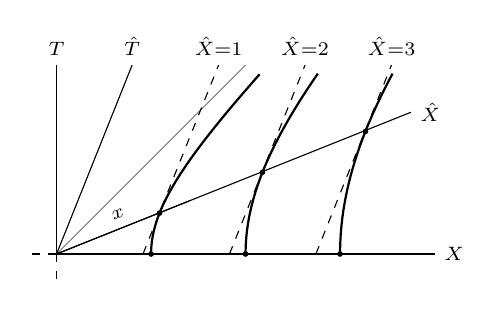
\begin{tikzpicture}[scale=1.2]
    \draw[color=gray] (0,0)--(2,2);
    \draw (0,0)--(4,0) node[right]{$\scriptstyle X$};
    \draw[dashed] (0,0)--(-0.3,0);
    \draw[dashed] (0,0)--(0,-0.3);
    \draw (0,0)--(0,2) node[above]{$\scriptstyle T$};
    \draw (0,0)--({1.3*sinh(0.42)*2.5},{1.3*sinh(0.42)}) node[midway,sloped,above]{$\scriptstyle x$};
    \draw (0,0)--(1.5*2.5,1.5) node[right]{$\scriptstyle\hat{X}$};
    \draw (0,0)--(0.8,0.8*2.5) node[above]{$\scriptstyle\hat{T}$};
    \draw[domain=0:1.4,thick,samples=100] plot({cosh(\x)},{sinh(\x)});
    \draw[domain=0:0.85,thick,samples=100] plot({2*cosh(\x)},{2*sinh(\x)});
    \draw[domain=0:0.6,thick,samples=100] plot({3*cosh(\x)},{3*sinh(\x)});
    \foreach \n in {1,2,3}{
    \fill (\n,0) circle(0.03);
    \fill ({\n*cosh(0.42)},{\n*sinh(0.42)}) circle(0.03);
    \draw[dashed] (\n*0.915,0)--(0.8+\n*0.915,0.8*2.5) node[above]{$\scriptstyle\hat{X}=\n$};}
    \end{tikzpicture}
    }
    \quad
    \subfloat[\centering 按 $A$ 相等分布]{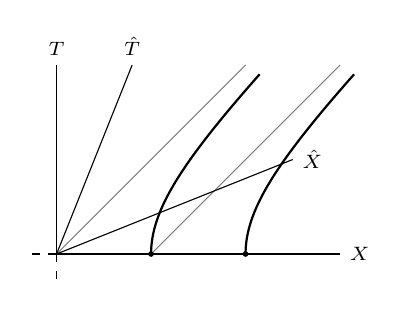
\begin{tikzpicture}[scale=1.2]
    \draw[color=gray] (0,0)--(2,2);
    \draw[color=gray] (1,0)--(3,2);
    \draw (0,0)--(3,0) node[right]{$\scriptstyle X$};
    \draw[dashed] (0,0)--(-0.3,0);
    \draw[dashed] (0,0)--(0,-0.3);
    \draw (0,0)--(0,2) node[above]{$\scriptstyle T$};
    \draw (0,0)--(2.5,1) node[right]{$\scriptstyle\hat{X}$};
    \draw (0,0)--(0.8,0.8*2.5) node[above]{$\scriptstyle\hat{T}$};
    \draw[domain=0:1.4,thick,samples=100] plot({cosh(\x)},{sinh(\x)});
    \draw[domain=0:1.4,thick,samples=100] plot({cosh(\x)+1},{sinh(\x)});
    \fill (1,0) circle(0.03);
    \fill (2,0) circle(0.03);
    \end{tikzpicture}
    }%
    \caption{\small 欧氏空间中向心加速率恒为 $a$、匀速率 $v=1$ 转动的质点将走 $X^2+Y^2=R^2$ 且 $a=1/R$,弧长为 $\ell=R\theta$。从而预料,物体在加速率恒定时经伪转动走 $X^2-T^2=x^2$ 且 $A=1/x$,固有时为 $\tau=x\theta$。若观者按 $A=1/x$ 分布,则在共动系看来间距恒定,因为 $\d t = 0$ 时 $\d s^2 = \d x^2$。但若各观者 $A$ 一致,则双曲线成平移关系,间距不恒定,不同于 Newton 力学。}
\end{figure}

\subsection{Lorentz 变换推导*}\label{sec:PoincareLorentz}

本节旨在补上任意 Lorentz 变换的代数证明。由于重点只在矩阵的行列指标,故本节将上标都写作下标以简化运算。
根据相对性原理,对 $\Lambda$ 的分类同样适用于相应 $\Lambda^{-1}$。当然,亦可直接证明之。注意 $|\Lambda^{-1}|=|\Lambda|^{-1}$,我们只需证明 $(\Lambda^{-1})_{00}=\Lambda_{00}$。
欲用 $\Lambda$ 表示 $\Lambda^{-1}$。由式 \eqref{Lorentz} 有
\eq{\label{eq:nA-1=nA}
    \eta_{\mu\nu}(\Lambda^{-1})_{\mu\sigma}=\eta_{\sigma\lambda}\Lambda_{\lambda\nu},
}
进而
\eq{\label{eq:1258}
    (\Lambda^{-1})_{\lambda\sigma}=\eta_{\mu\sigma}\Lambda_{\mu\nu}\eta_{\nu\lambda}.}
此即用 $\Lambda$ 表示 $\Lambda^{-1}$ 的方法,取其 $\sigma=\lambda=0$ 就有 $(\Lambda^{-1})_{00}=\Lambda_{00}=(\Lambda^\mathrm{T})_{00}$。

下面用 $\{x\},\{x'\}$ 的相对速度表示 Lorentz 变换。
我们说 $S'$ 系相对于 $S$ 的速度是 $u_i=\dv*{x_i}{t}$,是指 $S'$ 任意的相对静止的世界线在 $S$ 下测得的速度分量都是 $u_i$。显然这等价于研究 $S'$ 系的空间原点运动。反之,设 $S$ 系的空间原点在 $S'$ 下测得 $u'_i=\dv*{x'_i}{t'}$。先考虑 $S'$ 的空间原点,其世界线始终满足 $\d x'_i=0$,则 $\d x_\lambda=(\Lambda^{-1})_{\lambda 0}\d x'_0$,故 $\Lambda_{00}=(\Lambda^{-1})_{00}=\dv*{t}{t'},(\Lambda^{-1})_{i0}=u_i\dv*{t}{t'}$,
    据式 \eqref{eq:nA-1=nA} 有 $\eta_{\mu\nu}(\Lambda^{-1})_{\mu\sigma}(\Lambda^{-1})_{\nu\lambda}={\eta}_{\sigma\lambda}$,    取 $\sigma=\lambda=0$ 有 $(\Lambda_{00})^2=1+\delta_{ij}(\Lambda^{-1})_{i0}(\Lambda^{-1})_{j0}$。
    再结合正时条件有 $\Lambda_{00}=(\Lambda^{-1})_{00}=\gamma$,以及 $(\Lambda^{-1})_{i0}=\gamma u_i$,其中 $u:=\sqrt{u_i u_i}$。再考虑 $S$ 的空间原点,类似地有 $\Lambda_{00}=\dv*{t'}{t},\Lambda_{i0}=u'_i \dv*{t'}{t}=\gamma u'_i$,
    以及
    \eq{
        u'_iu'_i=u_i u_i=u^2.
    }
    这看似是显然的,但现在要作为经过证明的结论。
    不过,这是用 $u'_i$ 表示 $\Lambda$,固然渴望用 $u_i$ 直接表示。对 \eqref{eq:1258} 其余 $\sigma,\lambda$ 值讨论有 $(\Lambda^{-1})_{i0}=-\Lambda_{0i},(\Lambda^{-1})_{0i} =-\Lambda_{i0}$,
    以及 $(\Lambda^{-1})_{ij}=(\Lambda^\mathrm{T})_{ij}$。
    可得 $\Lambda_{0i}=(\Lambda^\mathrm{T})_{i0}=-\gamma u_i$。

    还差 $\Lambda_{i0},\Lambda_{ij}$。尝试用 $u_i$ 表示 $u'_i$。取 \eqref{Lorentz} 式 $\sigma=0,\lambda=k$(反之亦可),有
    \eq{\label{eq:Au'=u}
        \delta_{ij}\Lambda_{i0}\Lambda_{jk}=\Lambda_{00}\Lambda_{0k}\implies \Lambda_{jk} u'_j=-\gamma u_k.
    }
    同理取 $\eta_{\mu\nu}\Lambda_{\sigma\mu}\Lambda_{\lambda\nu}={\eta}_{\sigma\lambda}$ 的 $\sigma=0,\lambda=k$ 有
    \eq{\label{eq:Au=u'}
        \Lambda_{kj} u_j=-\gamma u'_k.
    }
    故只需关注 $\Lambda_{ij}$。更直观的表示可利用 $R\in\mathrm{SO}(3)$。若两坐标系仅差一个旋转变换,则仍相对静止,相对论的动力学效应不会体现。boost 变换即指这类相对速度可朝任意方向的 Lorentz 变换,但保持空间坐标轴平行。二维特殊情形保持 $y'=y,z'=z$。boost 变换是“时空旋转”,故任意 Lorentz 变换应可表为一个 boost 变换和一个空间旋转的复合(因此不一定有 $u_i=-u'_i$)。为找到 $R$,注意总可假设
    $R_{ij}=:\Lambda_{ij}+S_{ij}$,
    其中 $\Lambda_{ij}$ 的符号取正是为迎合固有条件。由定义,$R_{ij}$ 满足
    \eq{
        \delta_{ik} R_{ij} R_{kl}=\delta_{jl},\quad R_{ij} u_j=-u'_i,\quad R_{ij} u'_i=-u_j.
    }
    取 \eqref{Lorentz} 式 $\sigma=j,\lambda=l$ 有 $\delta_{ik}\Lambda_{ij}\Lambda_{kl}=\delta_{jl}+ \gamma^2 u_j u_l$,
    结合式 \eqref{eq:Au'=u},\eqref{eq:Au=u'} 以及上式,经过一些繁琐计算后可得 $S_{ij}=\frac{\gamma-1}{u^2}u'_i u_j$,综上任意 Lorentz 变换可表为
    \eq{
        \Lambda_{00}=\gamma,\quad\Lambda_{0i}=-\gamma u_i,\quad\Lambda_{i0}=-\gamma R_{ij} u_j,\quad \Lambda_{ij}=R_{ij}+\frac{\gamma-1}{u^2}  R_{ik} u_k u_j.
    }
    取 $R_{ij}=\delta_{ij}$ 就可得任意 boost 变换
    \eq{
\Lambda_{00}=\gamma,\quad \Lambda_{0i}=\Lambda_{i0}=-\gamma u_i,\quad \Lambda_{ij}=\delta_{ij}+\frac{\gamma-1}{u^2}u_iu_j.
}
再令 $u_2=u_3=0$ 就有 $\Lambda_{11}=\Lambda_{00}=\gamma, \Lambda_{01}=\Lambda_{01}=-\gamma u_1$,即二维 boost 变换,常记作 $\Lambda(\theta)$。鉴于此,任意 Lorentz 变换可用 $R_{1},R_{2}\in\mathrm{SO}(3)$ 表为 $R_{1} \Lambda(\theta) R_{2}$ 的形式。

\section{广义相对论}
\subsection{引力度规}

引力场强正是试验质点加速度,加速度又恰是运动学概念,仅涉及时空坐标;另一方面,由于涉及运动坐标系,局域惯性系必将完整涉及 4 个坐标。可见四维时空很适合用于描述引力。
先考虑试验粒子在外场中的运动。根据等效原理,试验粒子的\textbf{最小引力耦合}(minimal gravitational coupling)即要求在局域惯性系中还原回狭义相对论。置自由落体质点,世界线在某局域惯性系 $\{\xi\}$ 中表为 $\xi^\alpha(\tau)$,则
\eq{
    \delta\int\d\tau=\delta\int\sqrt{-\eta_{\alpha\beta}\d\xi^\alpha\d\xi^\beta}=0\implies \tilde A^\alpha=\dv{\tilde{U}^\alpha}{\tau}=\dv[2]{\xi^\alpha}{\tau}=0.
}
考虑任意坐标系 $\{x\}$。注意 4-速表为 $U^\mu=\pdv{x^\mu}{\xi^\alpha}\tilde U^\alpha=\dv*{x^\mu}{\tau}$,则
\eq{
    A^\lambda=\pdv{x^\lambda}{\xi^\alpha}\tilde A^\alpha=\pdv{x^\lambda}{\xi^\alpha}\dv{\tau}(\pdv{\xi^\alpha}{x^\mu}U^\mu)=\dv{U^\lambda}{\tau}+\Gamma^\lambda_{\mu\nu}U^\mu U^\nu=0,
}
其中
\eq{\label{Christoffel}
\Gamma^\lambda_{\mu\nu}:=\pdv{x^\lambda}{\xi^\alpha}\pdv{\xi^\alpha}{x^\mu}{x^\nu}}
称为\textbf{Christoffel 符号},简称\textbf{克氏符}。微积分学的 Fubini 定理指出,任意坐标均有 $\del_{[\mu}\del_{\nu]}=0$,因此有 $\Gamma^\lambda_{[\mu\nu]}=0$。
同理,固有时满足
\eq{\label{eq:metric}
    \d\tau^2=-g_{\mu\nu}\d x^\mu\d x^\nu,\quad g_{\mu\nu}:= \eta_{\alpha\beta}\pdv{\xi^\alpha}{x^\mu}\pdv{\xi^\beta}{x^\nu}.
}
此即\textbf{时空度规}或\textbf{Lorentz 度规}。光属于电磁或量子实验的内容,也符合等效原理。
取参数 $\lambda:=\xi^0$,同理得
\eq{
    \dv[2]{x^\kappa}{\lambda}+\Gamma^\kappa_{\mu\nu}\dv{x^\mu}{\lambda}\dv{x^\nu}{\lambda}=0,\quad g_{\mu\nu}\dv{x^\mu}{\lambda}\dv{x^\nu}{\lambda}=0.
}

可从度规计算出克氏符。为构造克氏符定义式 \eqref{Christoffel},应对度规定义式 \eqref{eq:metric} 求坐标偏导:
\eq{\label{eq:g=gamma}
g_{\mu\nu,\lambda}=\Gamma^\rho_{\lambda\mu}g_{\rho\nu}+\Gamma^\rho_{\lambda\nu}g_{\rho\mu},
}
其中注意 $\eta_{\alpha\beta,\lambda}=0$。为从中提出克氏符,做指标轮换便可合并同类项。做轮换 $\mu\to\nu\to\sigma\to\mu$ 再消元得 $g_{\sigma\nu,\mu}+ g_{\mu\sigma,\nu}-  g_{\mu\nu,\sigma}=2g_{\sigma\lambda}\Gamma^\lambda_{\mu\nu}$。两边与 $g^{\sigma\alpha}$ 缩并可移项,再将 $\alpha$ 换回 $\lambda$ 就有
\eq{\label{eq:chris}
\Gamma^\lambda_{\mu\nu}=\frac{1}{2}g^{\sigma\lambda}\left(g_{\sigma\nu,\mu}+ g_{\mu\sigma,\nu}-  g_{\mu\nu,\sigma}\right).
}
由此快速证明 Poincaré 变换的仿射性:任意惯性系下克氏符全零,则 $\pdv{x'^\alpha}{x^\mu}{x^\nu}=\Gamma^\lambda_{\mu\nu}\pdv{x'^\alpha}{x^\lambda}=0$。
也可通过一般坐标系下的作用量得到运动方程。由等效原理知
\eq{
    \delta\int\sqrt{-g_{\mu\nu}\d x^\mu \d x^\nu}=0.
}
由 $L=-\sqrt{-g_{\mu\nu}\dot x^\mu\dot x^\nu}$ 计算得 $\pdv*{L}{\dot x^\kappa}=g_{\kappa\lambda}\dot x^\lambda$ 和 $\pdv*{L}{x^\kappa}=\frac{1}{2}g_{\mu\nu,\kappa}\dot x^\mu\dot x^\nu$,
则 E-L 方程是
\eq{
\ddot x^\lambda+\frac 12g^{\kappa\lambda}\left(2g_{\kappa\nu,\mu}-g_{\mu\nu,\kappa}\right)\dot x^\mu\dot x^\nu=0\implies \ddot x^\lambda+\Gamma^\lambda_{\mu\nu}\dot x^\mu\dot x^\nu=0,
}
最后一步是注意 $g_{\kappa\nu,\mu}\dot x^\mu\dot x^\nu=g_{\kappa(\mu,\nu)}\dot x^\mu\dot x^\nu$。再重参数化即可。

克氏符没有错开指标书写是考虑到一般不会混淆,且它其实是赝张量:
\begin{align} \Gamma_{\mu \nu}^{\prime \lambda} &= \frac{\partial x^{\prime \lambda}}{\partial \xi^\alpha} \frac{\partial^2 \xi^\alpha}{\partial x^{\prime \mu} \partial x^{\prime \nu}}=\frac{\partial x^{\prime \lambda}}{\partial x^\rho} \frac{\partial x^\rho}{\partial \xi^\alpha} \frac{\partial}{\partial x^{\prime \mu}}\left(\frac{\partial x^\sigma}{\partial x^{\prime \nu}} \frac{\partial \xi^\alpha}{\partial x^\sigma}\right)\nonumber\\ 
    & =\frac{\partial x^{\prime \lambda}}{\partial x^\rho} \frac{\partial x^\rho}{\partial \xi^\alpha}\left(\frac{\partial x^\sigma}{\partial x^{\prime \nu}} \frac{\partial x^\tau}{\partial x^{\prime \mu}} \frac{\partial^2 \xi^\alpha}{\partial x^\tau \partial x^\sigma}+\frac{\partial^2 x^\sigma}{\partial x^{\prime \mu} \partial x^{\prime \nu}} \frac{\partial \xi^\alpha}{\partial x^\sigma}\right)\nonumber\\
&=\frac{\partial x^{\prime \lambda}}{\partial x^\rho} \frac{\partial x^\tau}{\partial x^{\prime \mu}} \frac{\partial x^\sigma}{\partial x^{\prime \nu}} \Gamma_{\tau \sigma}^\rho+\frac{\partial x^{\prime \lambda}}{\partial x^\rho} \frac{\partial^2 x^\rho}{\partial x^{\prime \mu} \partial x^{\prime \nu}},
\end{align}
可见多出一项。$\Gamma^{\lambda}_{\mu\nu}$ 是坐标系自身信息。比如,平面上的测地线是直线,但是克氏符仍可非零,只要选择复杂的坐标系即可。

\begin{figure}[ht]
    \centering
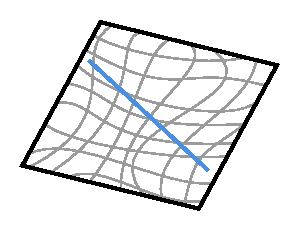
\includegraphics[width=.4\textwidth]{fig/chpt01/geodesic.pdf}
    \caption{ $\R^2$ 任意坐标系及直线}
\end{figure}

引力作用现解释为度规非闵。因为倘若存在某系使得处处 $g_{\mu\nu}=\eta_{\mu\nu}$,该系就为惯性系,而自由粒子运动为直线,说明无引力。可见即使克氏符是赝张量,其实也能体现绝对的引力现象,因为度规非闵等价于\textit{不存在}坐标系使克氏符\textit{处处}为零。只保证存在局域惯性系使克氏符严格在测地线上全零。
引力场可由时空度规描述,而前文提过,度规决定一套几何学,故\textit{引力可表为时空的几何效应},即\textbf{Lorentz几何}。
Poincaré 和 Riemann 都尝试过仅用空间几何构建引力理论,但未能成功。引力几何理论的关键就在于补上时间这一维,时间对引力亦有贡献。

测地线方程指出 $\Gamma^{\lambda}_{\mu\nu}$ 具有引力场强的意义,进而 $g_{\mu\nu}$ 具有引力势的意义。实际上的确可直接寻找度规同引力势的关系。
置一孤立场源。
研究时坐标系可取为与场源共动,比如地面系或某个遥远观者所尽可能构造的坐标系。
注意孤立系统各不影响,因而所关心场源的外引力场很弱,则该系近似为惯性系的余地很大。
并且,当远离所关心的孤立系统时,引力场是\textbf{渐弱的},即任取某种距离 $r$(如欧氏距离)后有 $g_{\mu\nu}=\eta_{\mu\nu}+O(r^{-1})$。
当然,也可直接考虑的场源质量较小。可见无论如何,都能考虑\textbf{线性近似},即与 $\eta_{\mu\nu}$ 只差小量:
\eq{
    g_{\mu\nu}=\eta_{\mu\nu}+h_{\mu\nu},\quad |h_{\mu\nu}|\ll 1.
}
从而能在 $\eta_{\mu\nu}$ 的惯性系中将引力近似解释为 $h_{\mu\nu}$。在弱场意义上,假若所研究的对象还\textbf{低速},即 $h_{\mu\nu,0}=0$ 且试验质点近似静止,便可认为 Newton 理论成立。
这其实也是对一套新理论的基本要求,称为\textbf{Newton 极限}。
由归一性知
\eq{
    U^\mu=(-g_{00})^{-1/2}\delta^\mu_0,
}
从而一阶意义上 $U^\mu=\delta^\mu_0$。此时测地线方程为 $\dv*{U^\mu}{\tau}=-\Gamma_{00}^\mu= \frac 12 g^{\mu\nu} g_{00,\nu}=\frac 12 \eta^{\mu\nu} h_{00,\nu}$,则 $-\del^i\phi=\dv*[2]{x^i}{t}=\frac 12 \delta^{ij} h_{00,j}$,故
\eq{
    h_{00}=-2\phi,\quad g_{00}=-(1+2\phi),
}
其中规定 $h_{\mu\nu},\phi$ 在无穷远处均衰减至零。


\subsection{Levi-Civita 联络}\label{sec:co-di}

可以看到 $\dv*{U^\lambda}{\tau}$ 或偏导数只有 Lorentz 协变性而无广义协变性。我们将 4-加速理解为对 4-速求一种保持张量协变性的导数,这种导数只在局域惯性系中才还原为 ${\d\tilde U^\alpha}/{\d\tau}$。不妨记 $D/\d\tau$,即 $A^\lambda={D U^\lambda}/{\d\tau}=\dv*{U^\lambda}{\tau}+\Gamma^\lambda_{\mu\nu}U^\mu U^\nu$。
$D$ 称为\textbf{绝对微分}或\textbf{协变微分},日文译为\textbf{共变}。$D/\d\tau$ 称为\textbf{沿线协变导数}。换言之 $D/\d\tau$ 总保持其作用对象的广义协变性,而只在局域惯性系中还原回 $\d/\d\tau$。
相应于 $\dv*{\tau}$ 可按全微分关系表为若干坐标偏导 $\del_\nu$ 的线性组合,对 $D/\d\tau$ 而言亦有\textbf{协变导数} $\nabla_\mu$ 的概念\footnote{注意与规范协变导数 $D_\mu$ 相区分。}。一般只讨论张量的协变导数。比如对逆变矢量 $V^\mu$ 而言有 ${D V^\mu}/{\d\tau}=:\nabla_\nu V^\mu {\d x^\nu}/{\d \tau}=U^\nu\nabla_\nu V^\mu$,且可有类似的分号简记:$V^\mu{}_{;\nu}=\nabla_\nu V^\mu :={V^\mu}{}_{,\nu}+\Gamma^\mu_{\sigma\nu}V^\sigma$。常把多出的克氏符项称为对偏导数的“协变性修正”。
协变导数的优势是无需借助于曲线及其参数,但劣势是某点的 $ V^\mu{}_{;\nu}$ 要求 $V^\mu$ 在该点邻域都有定义,而沿线求导只要求曲线上的邻域有定义。

其它张量的协变导数仍可从局域惯性系出发,按张量变换律推出,但更简单地关注如下事实:首先,就标量 $f$ 而言,由全微分或链式法则可知,偏导已有广义协变性,故 $f_{;\nu}=f_{,\nu}$。
其次,从局域惯性系的偏导可知,任意协变导数应具有\textbf{Leibniz 法则},便可从标量、逆变矢量的协变导数及 Leibniz 法则推出一般情形。首先就协变矢量而言,构造标量 $V^\mu\omega_\mu$,则对任意 $V^\mu$ 有 $(V^\mu\omega_\mu)_{;\nu} = (V^\mu\omega_\mu)_{,\nu} $,用 Leibniz 法则拆项并代入矢量协变导数有 $V^\mu \omega_{\mu;\nu}+\omega_{\mu}\Gamma^\mu_{\nu\sigma}V^\sigma=V^\mu(\omega_{\mu;\nu}+\Gamma^\sigma_{\mu\nu}\omega_{\sigma})=V^\mu \omega_{\mu,\nu}$,因此 $\omega_{\mu;\nu}=\omega_{\mu,\nu}-\Gamma^\sigma_{\mu\nu}\omega_\sigma$。
按此方法可得 $(k,l)$-张量的协变导数为
\begin{align}\label{eq:cov-tens}
     T^{\mu_1\cdots\mu_k}{}_{\nu_1\cdots\nu_l;\lambda}&=
      T^{\mu_1\cdots\mu_k}{}_{\nu_1\cdots\nu_l,\lambda}\nonumber\\
&+\sum_{i=1}^k \Gamma^{\mu_i}_{\lambda \sigma} T^{\mu_1\cdots\sigma\cdots\mu_k}{}_{\nu_1\cdots\nu_l}-\sum_{j=1}^l\Gamma^{\sigma}_{\lambda \nu_j} T^{\mu_1\cdots\mu_k}{}_{\nu_1\cdots\sigma\cdots\nu_l}.
\end{align}
在记忆时注意,此即先填上一个偏导,再对所有指标依次添加相应的克氏符修正项(正负取决于指标上下),并满足指标平衡。

式 \eqref{eq:g=gamma} 说明度规的协变导数为零:$g_{\mu\nu;\sigma}= {g_{\mu\nu,\sigma}}-g_{\mu\lambda}\Gamma^\lambda_{\sigma\nu}-g_{\nu\lambda}\Gamma^\lambda_{\sigma\mu}=0$,
称为\textbf{度规适配性}(metric-compatibility)。进而可直接在任意坐标系下证明 $A^\mu,U^\nu$ 正交: $A^\mu U_\mu=\frac 12  \frac{D}{\d\tau} (g_{\mu\nu} U^\nu U^\mu)=0$。
数学上称满足 $D V^\mu/\d\tau=0$ 的逆变矢量 $V^\mu$ 在做\textbf{平行移动}(parallel transport)或\textbf{Levi-Civita 移动}。切矢 $T^\mu=\dv*{x^\mu}{\sigma}$ 沿其自身平行移动的曲线称为\textbf{测地线}(geodesic),即 $T^\mu\nabla_\mu T^\lambda =0$。
此称\textbf{测地线方程}。可见自由落体运动就是引力度规下的测地线。假设 $V^\mu,W^\nu$ 沿某条线平行移动,则内积沿线恒定:$\frac{D}{\d\tau}(V^\mu W_\mu)=0$。
就单个 $V^\mu$ 而言说明模方恒定,的确可看作一种“平行移动”。
\begin{figure}[ht]\centering
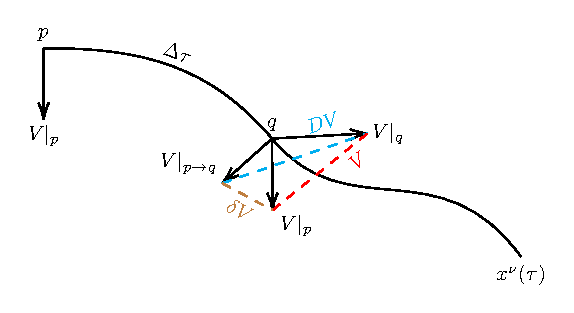
\includegraphics[width=.6\textwidth]{fig/chpt01/covar-deri.pdf}
    \caption{图中 $\Delta\tau$ 等差值均夸大}\label{covar-deri}
\end{figure}
不妨考察其直观含义。如图 \ref{covar-deri},设某曲线 $x^\nu(\tau)$ 上 $p$ 为参数零点,而邻近点 $q$ 的参数记作 $\Delta\tau$(可正可负)。若矢量场 $ V$ 至少在 $p,q$ 线段上有定义,便可讨论 $p$ 处沿线导数算符。设矢量场在 $p,q$ 分别取值 $ V|_p, V|_q$,则
\[\eval{\dv{V^\mu}{\tau}}_p=\lim_{\Delta\tau\to 0}\frac{V^\mu|_q-V^\mu|_p}{\Delta\tau}\]
是直接比较 $V|_q,V|_p$,但二者隶属不同切空间,差值 $\d V$ 意义不明。这是 $\d V^\mu/\d\tau$ 不协变的直观理解。欲画出 $\d V$,需将矢量照搬至同一点作差。不妨考虑 $q$ 点。图中 $q$ 点的 $V|_p$ 为照搬结果,故 $\d V$ 标注如图。另一方面,
\[\eval{\frac{DV^\mu}{\d\tau}}_p=\lim_{\Delta\tau\to 0}\frac{V^\mu|_q-V^\mu|_p}{\Delta\tau}+\Gamma^\mu_{\lambda\nu}|_p  V^\nu|_p \lim_{\Delta\tau\to 0} \frac{\Delta x^\lambda}{\Delta\tau}=\lim_{\Delta\tau\to 0}\frac{V^\mu|_q-V^\mu|_{p\to q}}{\Delta\tau},\]
其中 $V^\mu|_{p\to q}=V^\mu|_p-\Gamma^\mu_{\lambda\nu}|_p  V^\nu|_p \Delta x^\lambda$。
可见 $DV^\mu/\d\tau$ 是求 $V|_q$ 与 $q$ 处新矢量 $V|_{p\to q}$ 之差。这样 $D V$ 表为如图。$\delta V$ 为 $V|_{p\to q}, V|_p$ 之差。由上式或图示知 $\delta V^\mu = \d V^\mu-D V^\mu=-\Gamma^\mu_{\sigma\nu}V^\sigma\d x^\nu$,这便是克氏符项所给出的修正。$V|_{p\to q}$ 其实就是平移移动的结果。为看出这一点,只需令 $V$ 自己就处处按这种方式移动,则 $D V^\mu/\d\tau=0$。

设定时空上的逆变矢量场是给各时空点赋予其相应的逆变矢量,一个逆变矢量是绑定于一点的,故任意两点 $p,q$ 处各自的逆变矢量本无关联。然而给定某 $p,q$ 间之曲线,可通过矢量的平行移动,将两个切空间联系起来。因此 $\nabla_\nu$ 又被称为\textbf{联络}(connection)。附录 \ref{appx:curvature} 给出了一般的联络定义,每种联络都有相应的\textbf{联络系数} $\hat{\Gamma}^\lambda_{\mu\nu}$,相应测地线用 $U^\nu\hat\nabla_\nu U^\mu=0$ 定义。设\textbf{挠率}(torsion)为 $T^\lambda{}_{\mu\nu}:=2\Gamma^\lambda_{[\mu\nu]}$,它靠着克氏符作差消除了这一项,故是张量。按式 \eqref{Christoffel} 定义的联络系数满足 $T^\lambda{}_{\mu\nu}=0$,这种联络称为\textbf{无挠}(torsion-free)\textbf{联络}。度规适配的无挠联络称为\textbf{Levi-Civita 联络}。由此二条件可证联络系数正是克氏符,故 Levi-Civita 联络存在且唯一。
我们主要研究\textbf{无挠时空},必须选择 Levi-Civita 联络。一是出于方便,二是每一时空点都有局域的 Lorentz 不变性。若要求还要涵盖局域的平移对称性,即总地要求局域 Poincaré 对称性,需要考虑有挠联络。这仍能遵循等效原理,因为测地线方程中 $U^\mu U^\nu=U^{(\mu} U^{\nu)}$,只要求对称部分 $\Gamma^\lambda_{(\mu\nu)}$ 等于 \eqref{Christoffel} 式也仍使粒子在引力下走测地线。同理 $g_{[\mu\nu]}\ne 0$ 亦可,但为方便总选二阶对称张量作为度规。 

\subsection{广义不变性}

Einstein 想要借由广义协变性发展出一套坐标选择无关的理论,以\textit{尽可能排除人为因素}。但协变性对约束引力理论是不够的,事实上还需要不变性。首先,将 Lorentz 不变性中的常数不变推广到所谓的\textbf{绝对对象}(absolute object),即与物质状态无关的各种量,除了常数 $c=G=1,\hbar/2$,最重要的是还包括更高指标的,比如 Jacobi 矩阵元 $\pdv*{x^\mu}{x'^\nu}$。与物质状态有关而可变的称\textbf{动力学对象}(dynamical object),例如粒子的位置和动量、场的场强和能量密度等。给定任何物理方程,按定义总能把其中的量分为这两类。\textbf{广义不变性}就是说,\textit{任何物理定律有广义协变性,且方程中的绝对对象在任意坐标变换下相同},就能决定了哪些绝对对象才可以出现于方程中。
Jacobi 矩阵元这种一定是绝对对象的项就不能出现了。一个描述物理定律的方程必须是指标平衡的张量方程,才可在坐标变换下消除 Jacobi 矩阵元,进而一种坐标系对应方程的一种表达,并保持广义不变性,不会同时出现两种坐标系符号。

广义不变性所提出的要求当然高于 Lorentz 不变性。
$c=1,\hbar$ 和 $\eta_{\mu\nu}$ 有资格成为 Lorentz 不变性下的绝对对象,但 $\eta_{\mu\nu}$ 不能在任意坐标变换下严格不变,它可变成某个 $g_{\mu\nu}$。在引力理论中,由于 $g_{\mu\nu}$ 必须出现,我们只能期望 $g_{\mu\nu}$ 是动力学对象,它所满足的某个方程才能有广义不变性。结合等效原理,我们知道这是物质源产生引力场的定量关系,称为\textbf{引力场方程}或\textbf{场方程}。当今主流上称这套理论为\textbf{广义相对论}。当然,最初他认为“广义相对”一词来自广义协变性,但现在看来是来自等效原理和广义不变性。为避免歧义,Wheeler 很早就提议将该理论称为\textbf{几何动力学}(geometrodynamics)以强调其本质,即与物质相互作用的动力学几何。 

正如运动方程是 $x^\mu(\tau)$ 的常微分方程,场方程是 $g_{\mu\nu}$ 的偏微分方程,且根据广义不变性,它应是张量方程,其中的张量由度规及其偏导构造。记自由引力场、物质场的总拉氏密度为 $\mathcal L$。尽管可在局域惯性系中消除引力,但作为物理规律的作用量是不能在局域惯性系中失去耦合性的,它必须是标量场。取局域惯性系 $\{\xi\}$ 并置 $S=\int \mathcal L \d[4]{\xi}$。
体元变换 $\d[4]x =\tilde J \d[4]{\xi}$ 的 $\tilde J$ 能用度规行列式表示。记度规在 $\{x\}$ 系的行列式是 $g:=\det(g_{\mu\nu})$。对 $g_{\mu\nu}$ 的定义取行列式有
\eq{
    g=\det(\pdv{\xi^\alpha}{x^\mu})\det(\pdv{\xi^\beta}{x^\nu})\det(\eta_{\alpha\beta})=-\tilde J^{-2},
}
假设坐标变换保持右手性,则
\eq{
    \sgn g=-1\implies 1/\tilde J=\sqrt{-g}\implies S=\int \mathcal L \sqrt{-g}\d[4]{x},
}
可见 $g$ 虽与坐标选择有关,但在变换下一定保号,即引力度规的行列式总是负的(无关号差)。规定\textbf{适配体元} $D^4 x$ 只在局域惯性右手系 $\{\xi\}$ 中表为 $\d[4]\xi$,就有 $D^4 x=\sqrt{-g}\d[4]{x}$。
可以考虑用张量缩并获得标量。这种张量必须直接代表引力强弱,它不能是 $g_{\mu\nu}$ 级的,因为可用局域惯性系消为 $\eta_{\alpha\beta}$;也不能是 $g_{\mu\nu,\lambda}$ 级的,因为其可表为克氏符,在一点处可取局域惯性系使其为零。这意味着至少要考虑二阶导的构造,故最终场方程至少是二阶的。按有效性精神,先考虑有且仅有二阶的情形;且注意 Newton 引力论在低精度实验中是成立的,故广义相对论必须囊括这一理论,而 Poisson 方程恰好也是二阶的。
然暂不清楚将二阶导数作用于何物,因此要回到物理学。相比于单条测地运动,潮汐现象必须在足够大邻域内,等效原理不再适用。若欲寻求尽可能简单的定义,则该张量场\textit{在一点}就应具备潮汐意义。

\subsection{潮汐}

\begin{figure}[ht]\centering
    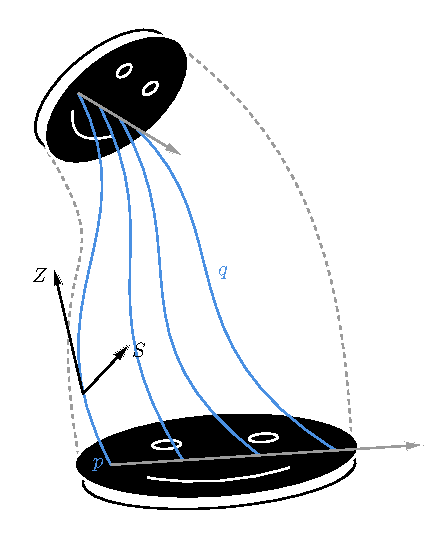
\includegraphics[width=.5\textwidth]{fig/chpt01/geo-devi.pdf}
            \caption{测地偏离}
            \label{fig:geo-devi}
\end{figure}
设物质场与引力场的最小耦合项为 $S_M=\int\mathcal L_M D^4{x}$,并通常令
\eq{
    S=S_G+S_M=\int\left(\frac{1}{2\kappa}\mathcal L_G +\mathcal L_M\right)\sqrt{-g}\d[4]{x},
}
其中 $\kappa$ 是按习惯设置的待定耦合常数。
为构造 $\mathcal L_G$,先找到具有潮汐意义的张量。考虑任意流体,如图 \ref{fig:geo-devi},对共动系的空间部分讨论如下。任选一条不自交的光滑曲线,使其上任一切矢都与过该点的观者相交,称为\textbf{横向曲线}。用 $s$ 参数化横向曲线,则与其相交的观者对应了交点参数,即在线汇中挑出了一个\textbf{单参族},横向曲线沿各观者 4-速便扫出一张 2 维曲面,可称\textbf{世界面}(worldsheet)。设任意坐标系 $\{x\}$,则可表为 $x^\mu(\tau,s)$,其中 $\{\tau,s\}$ 可以视为共动系的子集,当然也可不要求对钟,直接约定某初始的横向曲线 $x^\mu(0,s)$。可取单参族中的一者为\textbf{基准观者}(fiducial observer),比如 $x^\mu(\tau,0)$,而 $s$ 正方向的邻近观者称其\textbf{邻居}(neighbor),或者用\textbf{偏离矢量}(separation vector) $S^\mu:=\pdv*{x^\mu}{s}$ 来指代,其大小象征相对间距。这样 $x^\mu(\tau,s)$ 上建立了观者 4-速场 $Z^\mu:=\pdv*{x^\mu}{\tau}$ 和偏离矢量场 $S^\mu$。由链式法则,它们的确逆变。

再考虑类时测地线汇,其共动系可称\textbf{测地系}。相对加速度场表征为偏离矢量沿 4-速场的二阶协变导数 $Z^\nu \nabla_\nu(Z^\kappa \nabla_\kappa S^\lambda)$,部分书籍也采用记号 ${D^2S^\lambda}/{\d\tau^2}$。很容易展开证明 $Z^\nu\nabla_\nu S^\mu=S^\nu\nabla_\nu Z^\mu$,则
\begin{align}
    Z^\nu \nabla_\nu(Z^\kappa \nabla_\kappa S^\lambda)&= Z^\nu \nabla_\nu\left(S^\kappa\nabla_\kappa Z^\lambda\right) = \left(Z^\nu \nabla_\nu S^\kappa\right)\nabla_\kappa Z^\lambda+Z^\nu S^\kappa \nabla_\nu \nabla_\kappa Z^\lambda\nonumber\\
    &= \left(S^\nu \nabla_\nu Z^\kappa\right)\nabla_\kappa Z^\lambda+Z^\nu S^\kappa\left(\nabla_\kappa \nabla_\nu Z^\lambda+2\nabla_{[\nu}\nabla_{\kappa]}Z^\lambda\right)\nonumber\\
    &=S^\kappa\nabla_\kappa\left(Z^\nu \nabla_\nu Z^\lambda\right) +2Z^\nu S^\kappa\nabla_{[\nu}\nabla_{\kappa]}Z^\lambda\nonumber\\
    &=R^\lambda{}_{\mu\nu\kappa}  Z^\mu  Z^\nu S^\kappa,\quad R^\lambda{}_{\mu\nu\kappa}Z^\mu:= 2\nabla_{[\nu}\nabla_{\kappa]}Z^\lambda,
\end{align}
称为\textbf{测地偏离}(geodesic deviation)\textbf{方程},解 $S^\lambda$ 称为\textbf{Jacobi 场}。$R^\lambda{}_{\mu\nu\kappa}$ 表征潮汐形变程度,是 $g_{\mu\nu,\lambda\kappa}$ 级的张量:式左是协变导数,式右 $Z^\mu,S^\kappa$ 是逆变矢量。这称为\textbf{Riemann 张量}。
Jacobi 场固然无穷多种,但我们感兴趣满足对钟正交性的 Jacobi 场。实际上,任意 $S^\lambda$ 总可投影为正交 Jacobi 场
\eq{\eta^\lambda=S^\lambda+Z_\nu S^\nu Z^\lambda,}
而只要初始横向曲线与线汇正交,则此后都保持正交:$Z^\nu \nabla_\nu\left(S^\mu Z_\mu\right) =Z_\mu Z^\nu \nabla_\nu S^\mu=Z_\mu S^\nu \nabla_\nu Z^\mu=\frac{1}{2} S^\nu \nabla_\nu\left(Z_\mu Z^\mu\right)=0$。
可以展开定义式:计算 $\nabla_\nu\nabla_\kappa V^\lambda$ 时注意勿先展开内部,将 $\nabla_\kappa V^\lambda$ 视作整体以避开对克氏符求导,最后代入无挠性得
    \eq{\label{eq:Rie-cur}
         R^\lambda{}_{\mu\nu\kappa}:=-2\Gamma^\lambda_{\mu[\nu,\kappa]}+2\Gamma^\lambda_{\sigma[\nu} \Gamma^\sigma_{\kappa]\mu}.
    }
故 $R^\lambda{}_{\mu\nu\kappa}$ 表征度规的非闵程度。

再考虑 Newton 极限。取测地系 $\{\xi\}$ 并设正交 Jacobi 场 $\eta^\mu$。显然 $\tilde Z^\mu=\delta^\mu_0$ 且 $\tilde\eta^0=0$。根据定义显然有反称性
\eq{\label{eq:R_..ab=-}
    {R^\lambda}_{\mu\nu\kappa}={R^\lambda}_{\mu[\nu\kappa]},
}
则测地偏离方程在共动系下写作 $\pdv[2]{\tilde\eta^i}{t}=-\tilde R^i{}_{0 j 0} \tilde\eta^j$。
设每条测地线足够低速,故共动系成为了惯性系,进而 $\pdv[2]{\tilde\eta^i}{t}\approx \tilde\eta^j \pdv{\xi^j}\pdv[2]{\xi^i}{t}=-\tilde\eta^j \pdv{\xi^j}\tilde\del^i\phi$。
从而 $\tilde R^\sigma{}_{0 \sigma 0}=\tilde R^i{}_{0 i 0} \approx \tilde\partial_i\tilde\partial^i{\phi}$。可见 $R_{\mu\nu}:={R^\sigma}_{\mu\sigma\nu}$ 很有意义,称为\textbf{Ricci 张量}。
也可从 $g_{00}=-(1+2\phi)$ 及 $R_{\mu\nu}$ 定义得 $\tilde R_{00}=-\frac 12 \nabla^2 g_{00}=\nabla^2\phi$。
还可尝试展开。首先可证线性代数中的 Jacobi 公式:
\[
    \partial_\lambda g=\pdv{g}{g_{\sigma\nu}}g_{\sigma \nu,\lambda}=\pdv{(g\delta_\sigma^\mu)}{g_{\sigma\nu}}g_{\mu \nu,\lambda} =g^{*\gamma\mu}\pdv{g_{\sigma\gamma}}{g_{\sigma\nu}} g_{\mu \nu,\lambda}=gg^{\gamma\mu}\delta^\nu_\gamma g_{\mu \nu,\lambda}=g g^{\mu \nu} g_{\mu \nu,\lambda},
\]
其中 $(g^{*\mu\nu})$ 是 $(g_{\mu\nu})$ 的伴随,具有性质 $g\delta_\sigma^\mu=g_{\sigma\gamma}g^{*\gamma\mu}$ 和 $g^{*\mu\nu}=gg^{\mu\nu}$。注意伴随(转置)矩阵元是相应代数余子式,当然有 $\pdv*{g^{*\gamma\mu}}{g_{\sigma\nu}}=0$。进而\textbf{缩并克氏符}为
\eq{
\Gamma_{ \sigma\mu}^\sigma=\frac{1}{2} g^{\sigma \kappa}\left( g_{\sigma \kappa,\mu}+ 2 g_{\mu [\kappa,\sigma]}\right)=\frac{1}{2} g^{\sigma \kappa}  g_{\sigma\kappa,\mu}=\frac{1}{2g}\partial_\mu g=\partial_\mu\ln\sqrt{-g}.
}
故
\eq{
    R_{\mu\nu}=\Gamma^\sigma_{\mu\nu,\sigma}-(\ln\sqrt{-g})_{,\mu\nu}+(\ln\sqrt{-g})_{,\kappa}\Gamma^\kappa_{\mu\nu}-\Gamma^\kappa_{\sigma\mu}\Gamma^\sigma_{\kappa\nu}.
}
可有进一步的缩并,即 $R_{\mu\nu}$ 的迹
\eq{
    R:=R^\mu{}_\mu=g^{\mu\nu}R_{\mu\nu}.
}
此即一个足够简单的 $g_{\mu\nu,\lambda\kappa}$ 级的标量,称为\textbf{Ricci 标量}。

现可给出实验操作意义的局域惯性系的定量标准。数学上固然要求局域惯性系严格建立在测地线上:假若克氏符在邻域 $U$ 内等于零,则借助邻域按 \eqref{eq:Rie-cur} 式得在线上 $R^\lambda{}_{\mu\nu\kappa}=0$,矛盾。只要邻域足够大,$R^\lambda{}_{\mu\nu\kappa}$ 便可测量。但观者往往又需借助时空邻域进行实验,好在只要 $U$ 尺寸数量级远小于 $1/\sqrt{R}$,同时也远小于其测量精度时,即使时空范围未严格至测地线,但 $R^\lambda{}_{\mu\nu\kappa}$ 也在精度范围内为零。当然,若实验范围较大或仪器精度够高,还是可以测量潮汐,见 \ref{sec:eq-prin} 节。

最小耦合指出可取 $\mathcal L_G=R$。下面研究变分。为简便运算,选择对 $g^{\mu\nu}$ 而非 $g_{\mu\nu}$变分,则 $\var(R\sqrt{-g})$ 即涉及 $g^{\mu\nu},R_{\mu\nu},\sqrt{-g}$ 三个部分。
首先是 $\delta\sqrt{-g}$。注意 $\delta^{\mu}_{\nu}=g^{\mu\lambda}g_{\lambda\nu}$ 可得 $0=g^{\mu\lambda}\var g_{\lambda\nu}+g_{\lambda\nu}\var g^{\mu\lambda}$,故
\eq{
\var g=gg^{\mu\nu}\var g_{\mu\nu}=-g g_{\mu\nu}\var g^{\mu\nu},\quad \delta \sqrt{-g}=-\frac12\sqrt{-g}g_{\mu\nu}\delta g^{\mu\nu}.
}
其次计算 $\var R_{\mu\nu}$。取局域惯性系有 $\delta\tilde R_{\alpha\beta} = \tilde\del_\sigma(\delta\tilde\Gamma^\sigma_{\alpha\beta})-\tilde\del_\beta(\delta\tilde \Gamma^\sigma_{\alpha\sigma}) = \nabla_\sigma(\delta\tilde\Gamma^\sigma_{\alpha\beta})-\nabla_\beta(\delta\tilde \Gamma^\sigma_{\alpha\sigma})$。
注意,虽克氏符不是张量,但克氏符变分是张量(作差消去非协变部分),故任意坐标系下有如下\textbf{Palatini 公式}
\eq{
\delta R_{\mu \nu}=2\nabla_{[\lambda}\delta \Gamma_{\nu]\mu}^\lambda,
}
于是 $g^{\mu\nu}\var R_{\mu\nu}=2 \nabla_{[\lambda}( g^{\mu\nu} \delta \Gamma_{\nu]\mu}^\lambda) =2\nabla_\lambda(g^{\mu [\nu} \delta \Gamma_{\mu \nu}^{\lambda]})$,其积分为边界项,舍去后有
\eq{\var \int R\sqrt{-g}\d[4]{x} 
\simeq\int G_{\mu\nu} \var g^{\mu\nu} \sqrt{-g}\d[4]{x},\quad G_{\mu\nu}:=R_{\mu\nu}-\frac 12 g_{\mu\nu} R.}
$G_{\mu\nu}$ 称\textbf{Einstein 张量}。还可有 $G:=g^{\mu\nu}G_{\mu\nu}=R-\frac{1}{2}\delta^\mu_\mu R=-R\Rightarrow R_{\mu\nu}=G_{\mu\nu}-\frac 12 g_{\mu\nu} G$。这里没有引入物质场,因此自由引力场在最小耦合意义上满足 $G_{\mu\nu}=0$ 即 $R_{\mu\nu}=0$,称\textbf{真空方程}(vacuum equation)。闵氏度规显然是一个解。
真空方程已能描述很多引力现象,因为场源往往限制在很小的区域内,而外部区域真空,可允许试验粒子运动。

再考虑物质部分 $S_M$。约定 $\delta S_M =-\frac{1}{2} \int T_{\mu \nu} \delta g^{\mu \nu} D^4{x}$,即令
\eq{
T_{\mu \nu}:=-\frac{2}{\sqrt{-g}}\fdv{(\mathcal L_M\sqrt{-g})}{g^{\mu\nu}}=-2\fdv{\mathcal L_M}{g^{\mu\nu}}+g_{\mu\nu}\mathcal L_M,
}
则 $\var S\simeq\frac{1}{2\kappa}\int\left(G_{\mu\nu}-\kappa T_{\mu\nu}\right)\var g^{\mu\nu}\sqrt{-g}\d[4]{x}=0\Rightarrow G_{\mu\nu}=\kappa T_{\mu\nu}$,此即引力场方程的一般形式。可以预料 $T_{\mu\nu}$ 与场源质量(因而能量、动量)有关。还可有
\[ 
R_{\mu\nu}=G_{\mu\nu}-\frac 12 g_{\mu\nu} G=\kappa\left(T_{\mu\nu}-\frac12 g_{\mu\nu}T\right),
\]
称为\textbf{反迹}(trace-reversed)表达。当然,$T_{\mu\nu}$ 的具体意义和 $\kappa$ 的值还需落实。

\subsection{曲率的性质}

数学上称 $R^\lambda{}_{\mu\nu\kappa}$ 为\textbf{Riemann 内禀曲率}(intrinsic curvature)或\textbf{曲率}。$1/\sqrt{R}$ 相当于曲率半径。曲率为零时称度规为\textbf{平直的}(flat),非零时称\textbf{弯曲的}(curved),物理学可以借用这些词而称\textbf{时空曲率},时空分为\textbf{平直时空}和\textbf{弯曲时空}。渐弱度规也称\textbf{渐近平直}(asymptotically flat)度规。下面解释曲率称呼的意义。我们预先\textit{规定}欧氏空间是平直的,以它为基准可判断某条线、某张面的弯曲。考虑一个球面,其上任意切矢沿自身平移所得测地线即过球心的大圆。设从赤道某两处垂直延伸两条大圆弧,它们的间距逐渐缩短并交于极点。在一张平面上,初态平行的直线不可能改变间距。矢量平行移动就是相对于路径各处邻域平移,然而考虑将扇形围成圆锥面,矢量沿着包含尖端的环路平行移动后,与原矢量不重合,而直观上尖端处有曲率,故曲率非零时,平行移动结果往往与路径有关。
另一方面,按如下操作可计算球面上的线元:先用球坐标 $\{r,\theta,\phi\}$ 改写欧氏度规为
\eq{
    \d\l^2=\d r^2+r^2\d\Omega^2,\quad \d\Omega^2:=\d\theta^2+\sin^2\theta\,\d\phi^2,
}
当然,此处 $\Omega$ 不是立体角(solid angle),立体角满足的是 $\d\Omega=\sin\theta \d\theta\d\phi$。再取 $r=R$ 就有所谓的\textbf{球面度规} $\d\l^2=R^2\d\Omega^2$,由此可计算球面曲率不为零。像这样,约定背景空间中\textbf{嵌入}(imbedded)\textbf{曲面}的长度是用背景度规衡量的,这称为背景度规的\textbf{诱导}(induce)\textbf{度规}。可见度规在非欧或非闵时,内禀曲率非零而使测地间隔变化。但内禀曲率其实只由度规和坐标系计算而来,甚至无需嵌入某个高维背景来定义度规和曲率——对于四维时空,我们就只能抛弃嵌入思想来想象它。内禀曲率只反应内禀的弯曲程度而与曲面本身无关:球面在内禀意义下弯曲,但圆柱面在内禀意义下平直(借柱坐标发现诱导度规平直),尽管它在直观上弯曲。数学上,描述圆柱面这种对象的弯曲程度就需要嵌入思想,称为\textbf{外}(extrinsic)\textbf{曲率}。一个直观理解是,凡能连续地展平的曲面,尽管外曲率可不为零,但内禀曲率为零;真正不可连续展平的曲面内禀曲率、外曲率都非零。读者可观察纸塑地球仪是如何尝试将平面纸张大致贴合球面的。


曲率具有若干性质。首先注意无挠性导致 $\nabla_{[\nu}\nabla_{\kappa]}(V^\mu \omega_\mu)=0$,则可得
\eq{
    2\nabla_{[\nu}\nabla_{\kappa]} \omega_\mu = - R^\lambda{}_{\mu\nu\kappa} \omega_\lambda.
}
前文已提过反称性 \eqref{eq:R_..ab=-} 式,
其次是所谓的\textbf{Ricci 循环恒等式}(cyclic identities)
\eq{{R^\lambda}_{[\mu\nu\kappa]}=0.}
证明只需默认无挠性,并运用取测地系的技巧(其中 $\tilde R^\lambda{}_{\mu\nu\kappa}=-2\tilde \Gamma^\lambda_{\mu[\nu,\kappa]}$)。

\textbf{降指标 Riemann 曲率} $R_{\lambda\mu\nu\kappa}:=g_{\lambda\sigma}{R^\sigma}_{\mu\nu\kappa}$ 是一个常用概念,它与原先 ${R^\lambda}_{\mu\nu\kappa}$ 有等价的独立分量数,因此有时也称 Riemann 曲率。它使我们能看到更多性质,如反称性
\eq{
    R_{\lambda\kappa\mu\nu}=R_{[\lambda\kappa]\mu\nu}.
}
直接证明它亦可从无挠性和测地系入手。由此可知
$R_{\mu\nu}$ 是 ${R^\lambda}_{\mu\nu\kappa}$ 唯一非平凡缩并,另两种缩并是平凡的:$R^\sigma{}_{\mu\nu\sigma}=-R^\sigma{}_{\mu\sigma\nu}=-R_{\mu\nu}$,以及 $R^\sigma{}_{\sigma\mu\nu}=g^{\lambda\sigma}R_{\lambda\sigma\mu\nu}=g^{(\lambda\sigma)}R_{[\lambda\sigma]\mu\nu}=0$。
最后是前一对指标和后一对指标的对称性:
\eq{
    R_{\mu\nu\lambda\kappa}=R_{\lambda\kappa\mu\nu}.
}
同理默认无挠性并取测地系即可。包括式 \eqref{eq:R_..ab=-} 在内的这四条性质是我们能得到的所有代数性质了。

由 ${R^\lambda}_{\mu\nu\kappa}={R^\lambda}_{\mu[\nu\kappa]}$ 可知 Ricci 恒等式还有如下形式:
\eq{
    R^\lambda{}_{\mu\nu\kappa}+R^\lambda{}_{\nu\kappa\mu}+R^\lambda{}_{\kappa\mu\nu}=0.
}
注意,上式若存在相同指标,则总与另三条性质重复,故常考虑指标各不相同的非平凡 Ricci 恒等式。直观上,四维时空的 Riemann 曲率的分量有 $4^4=256$ 之多,但以上性质使其分量往往重复或为零。利用简单的组合数学可知其实际只有 20 个独立分量。由此还可证明,Riemann 曲率是唯一可由度规二阶导线性组合而成的张量。细节放入附录 \ref{appx:curvature}。故我们选择用 Riemann 曲率描述引力。

可用缩并将 Riemann 曲率进行压缩从而保留有用数据。前文已说明,初步缩并的唯一有用结果是 Ricci 曲率。可直接根据定义得
\eq{
    R_{\mu\nu}=R_{(\mu\nu)}.
}
亦可根据 $R_{\mu\nu\lambda\kappa}=R_{\lambda\kappa\mu\nu}$ 有 $R_{\mu\nu}=g^{\sigma\lambda}R_{\sigma\mu\lambda\nu}=g^{\sigma\lambda}R_{\lambda\nu\sigma\mu}=R_{\nu\mu}$。
此外,Ricci 标量也是非平凡缩并。虽然这不是唯一能从 $g_{\mu\nu},R^\lambda{}_{\mu\nu\kappa}$ 得到的非平凡标量(见附录 \ref{appx:curvature}),但确实是足够简单的一个。

除了上述纯代数性质之外,Riemann 曲率还满足一个微分恒等式:
\eq{
    R^\lambda{}_{ \mu [\sigma\nu ; \kappa]}=0,
}
这称为\textbf{Bianchi 恒等式}。可直接用无挠性和测地系证明之。
由 ${R^\lambda}_{\mu\nu\kappa}={R^\lambda}_{\mu[\nu\kappa]}$ 可知 Bianchi 恒等式还有如下形式:
\eq{
    R^\lambda{}_{ \mu \sigma\nu ; \kappa}+R^\lambda{}_{ \mu \nu\kappa;\sigma}+R^\lambda{}_{ \mu \kappa\sigma;\nu}=0.
}
对上式缩并 $\lambda,\sigma$ 再用 $g^{\mu\kappa}$ 升指标,且注意 $g^{\mu\kappa} R_{\lambda \mu\nu\kappa}=g^{\mu\kappa} R_{\mu\lambda\kappa \nu}=R^{\kappa}{}_{\lambda\kappa \nu}=R_{\lambda\nu}$,则 $\nabla^{\mu} R_{\mu\nu}+ \nabla^\lambda R_{\lambda\nu}-\del_\nu R=0\Rightarrow\nabla^{\mu} R_{\mu\nu}=\frac 12\del_\nu R$,故 $G_{\mu\nu}$ 无散:
\eq{
    \nabla^{\mu}G_{\mu\nu}=0.
}

\subsection{Einstein 方程}

考虑尘埃及其 4-速场 $Z^\mu$,
只需取局域惯性系即知质量守恒等价为 $\nabla_\nu(\mu^* Z^\nu)=0$。而协变散度可直接用偏导表示。
逆变矢量的散度为
\eq{
 V^\mu{}_{;\mu}= V^\mu{}_{,\mu}+\Gamma_{ \mu\nu}^\mu V^\nu=V^\mu{}_{,\mu}+V^\mu \partial_\mu\ln\sqrt{-g} =\frac{1}{\sqrt{-g}} \del_\mu\left(\sqrt{-g} V^\mu\right).
}
结论是任意系有 $\del_\nu(\mu^* Z^\nu\sqrt{-g})=0$,这给出 $\var(\mu^* Z^\nu\sqrt{-g})=0$ 的理由前文已述。
注意 $\var(Z^\mu Z_\mu)=\var(-1)=0$,则易得 $\var Z^\mu=\frac 12 Z_\nu \var g^{\mu\nu}$,故
\eq{
    \var(\mu^*\sqrt{-g})=\frac 12 \mu^* Z_\mu Z_\nu \sqrt{-g}\var g^{\mu\nu}\implies T_{\mu\nu}=\mu^* Z_\mu Z_\nu.
}
同理,可取 $\delta S_M =\frac{1}{2} \int T^{\mu \nu} \delta g_{\mu \nu} D^4{x}$ 而有
\eq{
T^{\mu \nu}:=\frac{2}{\sqrt{-g}}\fdv{(\mathcal L_M\sqrt{-g})}{g_{\mu\nu}}=2\fdv{\mathcal L_M}{g_{\mu\nu}}+g^{\mu\nu}\mathcal L_M=g^{\mu\alpha}g^{\nu\beta} T_{\alpha\beta}.
}
那么当然 $T^{\mu\nu}=\mu^* Z^\mu Z^\nu$。可见 $T^{00}=T_{00}=\mu$ 即能量密度,$T^{i0}=T^{0i}=\mu u^i $ 即动量密度或能流密度,而 $T^{ij}=\mu u^i u^j$ 即动流密度或应力张量。因此,$T^{\mu\nu}$ 称为物质场源的\textbf{4-动流密度}或\textbf{能动张量}(energy-momentum tensor)。$\nabla^{\mu}G_{\mu\nu}=0$ 要求
\eq{
    \nabla_\mu T^{\mu\nu}=0,
}
取 $\nu=0$ 即能量局域守恒,取 $\nu=i$ 即动量局域守恒。代入 $T^{\mu\nu}=\mu^* Z^\mu Z^\nu$,则 $\nabla_\mu T^{\mu\nu}=\mu^* Z^\mu\nabla_\mu Z^\nu$。故 $\nabla_\mu T^{\mu\nu}=0$ 等价于 $Z^\mu\nabla_\mu Z^\nu =0$,说明各质元自由落体。

考虑 Newton 极限。取共动系,$R_{\mu\nu}Z^\mu Z^\nu=\tilde R_{00}=\nabla^2\phi= 4\pi\mu^*$。另一方面 $\tilde Z^\mu=\delta^\mu_0,\tilde Z_\mu=-\delta_{\mu 0}$,则 $T_{\mu\nu}Z^\mu Z^\nu=\tilde T_{00}=\tilde T^{00}=\mu^*$。进而 $T:=g_{\mu\nu}T^{\mu\nu}=-T^{00}=-\mu^*$。由前文知 $R=-G=-\kappa T$,场方程与 $Z^\mu Z^\nu$ 缩并得 $4\pi\mu^*-\frac 12 (-1)\kappa \mu^*=\kappa\mu^*$,则
\eq{
    R_{\mu\nu}-\frac12 g_{\mu\nu} R=8\pi T_{\mu\nu},\quad \kappa=8\pi.
}
这称为\textbf{Einstein 方程}。$\frac{1}{16\pi}\int R \sqrt{-g}\d[4]{x}$ 称为\textbf{Einstein-Hilbert 作用量}。

\subsection{最小引力耦合}

现设流体带固有电荷密度 $\rho^*$,电流密度为 $J^\mu=\rho^* Z^\mu$。电荷守恒从局域惯性系出发变换为 $\nabla_\mu J^\mu = 0$,则后续对 $A_\mu,g^{\mu\nu}$ 的变分均有 $\var(J^\mu\sqrt{-g})=0$。
研究电磁场 $F_{\mu\nu}$ 的最小引力耦合。单粒子的运动方程遵循
\eq{
\delta\int \left(-m+q A_\mu U^\mu\right)\d\tau =0 \implies \frac{D P^\mu}{\d\tau}=q F^\mu{}_{\nu}U^\nu,
}
电磁场的运动方程遵循
\eq{
    \delta\int\left(-\frac{1}{16\pi} F^{\mu\nu} F_{\mu\nu}+A_\nu J^\nu\right)\sqrt{-g}\d[4]{x}=0 \implies \nabla_\mu F^{\mu\nu}=-4 \pi J^\nu,
}
而 $F_{\mu\nu}$ 的定义和无挠性自动给出 $F_{\mu\nu}=2\nabla_{[\mu}A_{\nu]}=2\del_{[\mu}A_{\nu]}$,则
\eq{
    F_{[\mu\nu;\lambda]}=F_{[\mu\nu,\lambda]}=0.
}
Lorenz 规范从局域惯性系出发变换为 $\nabla^\mu A_\mu =0$,则引力耦合的 d'Alembert 方程为
\begin{align}
    -4\pi J_\nu&=\nabla^\mu\nabla_\mu A_\nu- \nabla^\mu \nabla_\nu A_\mu = \nabla^\mu\nabla_\mu A_\nu- (\nabla_\nu\nabla^\mu A_\mu -g^{\kappa\mu} R^\lambda{}_{\mu\kappa\nu} A_\lambda)\nonumber\\
    &=\square_g A_\nu-g^{\mu\kappa} g^{\lambda\sigma} R_{\mu\sigma\kappa\nu} A_\lambda=\square_g A_\nu- R^\lambda{}_{\nu} A_\lambda,
\end{align}
其中 $\square_g:=\nabla^\mu\nabla_\mu$ 称为\textbf{Laplace-Beltrami 算子}。$g_{\mu\nu}$ 出现在克氏符中,以上都是$g_{\mu\nu},F_{\mu\nu}$ 的耦合方程。

由定义,电磁场的能动张量为
\eq{
T_{\mu\nu}=\frac{1}{4\pi}\left(F_{\mu\sigma}F_{\nu}{}^{\sigma}-\frac{1}{4}g_{\mu\nu} F_{\sigma\lambda}F^{\sigma\lambda}\right),
}
显然 $T=0$。以闵氏时空举例,电磁场在惯性系中所测能量密度为 $T^{00}=(\bm E^2+\bm B^2)/8\pi$;能流或动量密度为 $T^{i0}=-T_{i0}$ 即 Poynting 矢量 $(\bm E\times \bm B) / 4\pi$;动流密度或应力张量为 $T^{ij}=-(E^i E^j+B^i B^j)/4\pi+T^{00}\delta^{ij}$。代入 $\nabla_\mu F^{\mu\nu}=-4 \pi J^\nu$ 得
$\nabla^\mu T_{\mu\nu}=-F_{\nu\lambda}J^\lambda$。
设荷电介质为尘埃,则有\textbf{Einstein-Maxwell 作用量}
\eq{
    S=\int\left(\frac{1}{16\pi}(R - F^{\mu\nu} F_{\mu\nu})-\mu^*+A_\nu J^\nu\right)\sqrt{-g}\d[4]{x}.
}
然 $A_\mu$ 不参与度规变分,则能动张量只需加上 $\mu^* Z_\mu Z_\nu$。而运动方程为 $\mu^* Z^\mu\nabla_\mu Z^\nu=F^\mu{}_{\lambda}J^\lambda$,故电磁场和带电流体的总能动张量无散。上式关于 $g^{\mu\nu}$ 的变分结果为
\eq{
    R_{\mu\nu}-\frac12 g_{\mu\nu} R=2\left(F_{\mu\sigma}F_{\nu}{}^{\sigma}-\frac{1}{4}g_{\mu\nu} F_{\sigma\lambda}F^{\sigma\lambda}\right)+8\pi\mu^* Z_\mu Z_\nu.
}
称为\textbf{Einstein-Maxwell 方程}。

最小引力耦合基于等效原理。
可以看到以上弯曲时空中的电磁学方程,似乎都是将其平直情形做直接替换:
\[
    \eta_{\mu\nu}\to g_{\mu\nu},\quad\del_\mu\to\nabla_\mu,\quad\d\to D,
\]
故许多人将最小引力耦合理解为这种所谓的\textbf{最小替换}(minimal replacement)。必须指出这不一定成立,如 $-4\pi J_\nu=\square_g A_\nu- R^\lambda{}_{\nu} A_\lambda$ 就并非从 $\square A_\mu =-4\pi J_\mu$ 直接替换。
关键在于二阶及以上的协变导数将带来曲率效应,这不能用任何坐标系消除。能满足广义不变性的方程是很多的,不能冒然只做最小替换而图高枕无忧。企图从局域惯性系转化到一般坐标系的关键在于,导数内所作用的量\textit{全部}是广义不变的张量,显然 $\del^\nu(\del_\nu A_\mu)$ 括号内的 $\del_\nu A_\mu$ 并不满足。在一阶导时,可轻松保证导数作用的量是张量,故最小替换适用。这才是能从最小耦合推出最小替换的实质关键。

也有人将等效原理及其最小耦合理解为:若一个方程在平直情形时成立,则在弯曲情形也成立。这也是不一定的。的确,协变导数在平直时空的惯性系中表为偏导数。但曲率在平直情形直接为零,因此加上曲率额外项的方程也将符合这句话,比如 $\nabla_\mu F^{\mu\nu}+\alpha \nabla_\mu(F^{\mu\nu}R)=-4 \pi J^\nu$。但等效原理指的是,利用局域惯性系来描述真实引力场,这样才能排除 $\nabla_\mu(F^{\mu\nu}R)$。切记,这些张量和协变导数的定义是从局域惯性系中,做广义坐标变换得来。

或许有读者指出,具有曲率项的正确方程(如 $-4\pi J_\nu=\square_g A_\nu- R^\lambda{}_{\nu} A_\lambda$)也并不在局域惯性系中退回狭义相对论。对此,我们进一步指出最不容易混淆的正确理解:将最小耦合应用于一开始的作用量上。因为作用量始终是广义不变的标量,不涉及坐标变换等麻烦的过程,最小耦合只是引入了适配体元 $\sqrt{-g}\d[4]{x}$。故其实并不需要用局域惯性系去讨论一个物理方程,而只需要讨论最原始的作用量。

当然,并不一定要把等效原理、最小耦合奉为教条。
若在量子理论中非要讨论诸如 $\nabla_\mu(F^{\mu\nu}R)$ 的曲率项,可认为是在量子领域适当地放弃等效原理。但在经典理论的视角下,这些项的数量级太小,且目前实验精度无法达到(尤其是微弱的曲率),故等效原理仍被默认。总之,包括等效原理在内,最终都要接受实验的考验。


\subsection{规范自由与双曲性}

$g_{\mu\nu}$ 的独立分量有 $\binom{4+1}{2}=10$ 个,而仔细观察一下 Einstein 方程,任取坐标系 $\{x\}$ 把分量显式地展开,可发现 Einstein 方程是关于 $g_{\mu\nu}(x)$ 的二阶非线性偏微分方程组。即使给定边界条件,还不能完全确定 $g_{\mu\nu}$ 的具体表达。比如对于真空方程,由于自动满足 $\nabla^\mu G_{\mu\nu} = 0$,独立方程实际为 $10 - 4 = 6$ 个,不足以确定度规所有分量。显然若 $g_{\mu\nu}(x)$ 是一个解,则可通过坐标变换 $\{x\}\to \{x'\}$ 得到
\[
    g'_{\mu\nu}(x')=g_{\sigma\lambda}(x(x')){\pdv{x^\sigma}{x'^\mu}}(x'){\pdv{x^\lambda}{x'^\nu}}(x').
\]
由广义协变性,直接用 $x$ 去替换函数 $g'_{\mu\nu}(x')$ 中的 $x'$,也即直接去掉撇号,得到的 $g'_{\mu\nu}(x)$ 本就可作为 $\{x\}$ 系下 $g_{\mu\nu}(x)$ 之外一个新解。
换言之,度规解之间只能确定到相差 4 个任意函数,其暗含坐标变换的意义。
完全确定只需补充 4 个方程,称为\textbf{坐标条件}。
Einstein 曾为此困扰而企图放弃广义协变性,提出\textbf{空穴论证}(hole argument):设某时空区域内无物质,但存在由外部物质产生的引力场。取“坐标变换函数”在穴外为恒等变换,在穴内任意,则这说明外部确定的物质分布仍无法决定穴内“引力场”。
其错误在于混淆了引力场和度规。无论如何,引力场、物质场是客体实在,度规只是一种描述方法。
从被动观点来看,度规未变,坐标系是冗余的,则“新解”是同一度规在其它坐标系的值直接搬到现有坐标系下:
\begin{align*}
    \text{坐标系:}&\{\{x\},\{x'\},\{x''\}\cdots\},\\
    \text{旧度规 $g_{\mu\nu}$:}&\{g_{\mu\nu},g'_{\mu\nu},g''_{\mu\nu}\cdots\},\\
    \text{新度规 $\tilde g_{\mu\nu}$:}&\{g'_{\mu\nu},g''_{\mu\nu},\cdots\},
\end{align*}
而坐标系的物理实质已变。
我们的方程适于任意坐标系,故坐标条件可视为用于挑选特定坐标系。
从主动观点来看,我们认为产生了新度规,但它们在物理上等价,引力场仍一致,类似于描述同一电磁场的不同 $A^\mu$,这也被称为\textbf{广义相对论的规范自由性}。
换言之,主动观点认为坐标条件是度规的规范条件,而被动观点认为坐标条件用于约束坐标系。被动观点更通俗,更建议读者使用。

由于空穴论证中假设的坐标变换只发生在空穴中,因而 Einstein 开始讨论时空、坐标系在无物质时的存在性。最终他提出\textbf{点重合}(point coincidence)\textbf{原理}:\textit{各种可观测事件都归结为世界线的交叉点,物理理论是在预言这些交叉的分布}。物理预言在这种意义下当然具有坐标冗余性。在量子层面 Pauli 不相容似乎与之矛盾,只要将这种重合性理解为通过相互作用交换信息即可。当然,点重合其实还有更多的哲学意义未发掘,而这或许对量子引力的提出有帮助。
Kretschmann 借鉴 Leibniz 的相对关系主义,进一步提出\textbf{拓扑原理},即物质间的关系是拓扑性质的,实质上是引力场、物质场、时空都被一齐拖拽,而现实中看来,时空未动而坐标系变动。
这其实分别就是主动和被动观点。

对于有源方程,逻辑上自然想到是给定 $T_{\mu\nu}$ 后求解 $g_{\mu\nu}$,但实际上,$T_{\mu\nu}$ 的确切定义也需要 $g_{\mu\nu}$ 给定,比如 $Z^\mu Z_\mu = -1$。换言之,一般 $g_{\mu\nu}$ 同时出现于 $G_{\mu\nu},T_{\mu\nu}$ 中。因此整个方程的未知量除了 $g_{\mu\nu}$,实际上还包括描述物质场的物理量,比如电磁场 $F_{\mu\nu}$。故 Bianchi 恒等式 $\nabla^\mu T_{\mu\nu}=0$ 并不自动满足,而要视作额外约束。以尘埃为例,未知量 $g_{\mu\nu},\mu,Z^\mu$ 总共有 $10+4+1=15$ 个。另一方面,Einstein 方程、坐标条件和 4-速归一化提供了 $10+4+1=15$ 个独立方程。

坐标条件的任务本就是消除广义协变性带来的自由度,故当然不能是广义协变的等式。
一种常见的坐标条件是\textbf{波坐标条件}或\textbf{谐和坐标条件}\footnote{数学上 $\square f = 0$ 的解称为谐和(harmonic)函数。}:
\eq{
    \square_g x^\lambda=0\iff g^{\mu\nu}\Gamma^\lambda_{\mu\nu}=0,
}
其中 $x^\mu$ 按标量场处理。等价性只需展开:标量场的 Laplace-Beltrami 算子、2 阶张量的散度分别为
\begin{align}
    \square_g f&=\frac{1}{\sqrt{-g}} \del_\mu\left(\sqrt{-g} \nabla^\mu f\right)=\frac{1}{\sqrt{-g}} \del_\mu\left(\sqrt{-g} g^{\mu\nu}\del_\nu f\right),\\ 
T^{\mu \nu}{}_{;\nu}&=T^{\mu \nu}{}_{,\nu}+\Gamma_{\lambda \nu}^\mu T^{\lambda \nu}+\Gamma_{\lambda \nu}^\nu T^{\mu \lambda}
=\frac{1}{\sqrt{-g}} \del_\nu\left(\sqrt{-g} T^{\mu \nu}\right)+\Gamma_{\lambda \nu}^\mu T^{\lambda \nu},
\end{align}
进而 $\square_g x^\lambda=(-g)^{-1/2}\del_\mu(\sqrt{-g} g^{\mu\lambda})=-g^{\mu\nu}\Gamma^\lambda_{\mu\nu}$。
在谐和坐标条件下,经过冗长计算发现 Einstein 方程呈 $\square_gg_{\mu\nu}=N_{\mu\nu}$ 的形式,其中 $N_{\mu\nu}$ 是度规及其一阶导的非线性表达式。偏微分方程常见类型有椭圆型方程(如 Poisson 方程)、抛物型方程(如热传导方程)和双曲型方程(如波动方程)。考虑到 Lorentz 度规的号差,该方程组属于数学上的\textbf{拟线性}(quasilinear)\textbf{波动方程}。




方程的双曲性带来两个重要话题。第一是 Cauchy 适定问题,也即动力学问题。\textbf{适定性}是指给定适当的\textbf{初值条件}(某 $\Sigma_t$ 上的 $g_{\mu\nu},g_{\mu\nu,0}$),必存在唯一的解。换言之,给定初值后,研究场方程能否确定时空度规的未来演化。下面要说清方程细节。首先由 Bianchi 恒等式得
$\del_0 G^{\mu 0} =-\del_i G^{\mu i} - \Gamma^\mu_{\lambda\nu} G^{\lambda\nu} - \Gamma^\nu_{\lambda\nu} G^{\mu\lambda}$,
这不含度规的三阶及更高阶时间偏导,故 $G^{\mu 0}$ 至多只含 $g_{\mu\nu,0}$,即 $G^{\mu 0} =\kappa T^{\mu 0}$ 只能用以约束初值条件,从而动力学方程只剩 $G^{ij} =\kappa T^{ij}$,以确定 $g_{ij,00}$。剩下 $g_{0\mu,00}$ 由坐标条件确定即可,从而可代数或数值地求解方程。
第二是引力波。Einstein 本人在 1918 年就关注到方程的波动性,并认为存在波动解。在以后章节中,我们会证明其存在性,并说明其传播速度为光速。

\subsection{球对称黑洞}

首要任务是研究理想质点引力场。以一质点为空间坐标原点,观测结果建议\textit{质点引力场呈空间球对称}(spherical symmetry):存在坐标系 $\{\bar t,\bar r,\theta,\phi\}$,空间部分为正交球坐标系,且变换 $\theta\mapsto -\theta,\phi\mapsto -\phi$ 保持度规形式,则对经纬度只存在 $\d\theta^2,\d\phi^2$ 项;$\Sigma_{\bar t}$ 内任意 $\bar r$ 球面的诱导度规为 $K(\bar t,\bar r)\d\Omega^2$;其余分量只与 $\bar t,\bar r$ 有关\footnote{此形式在数学上属于\textbf{扭曲积}(warped product):度规可分离为 2 维和 $(n-2)$ 维部分:$g_{ab}(x^0,x^1)\d x^a\d x^b+K(x^0,x^1)\hat g_{ij}(x^2,\cdots,x^{n-1})\d x^i\d x^j$,其中 $ab$ 取 $0,1$;$ij$ 取 $2,\cdots,n-1$。}:
\[\d s^2=\bar g_{00}\d\bar t^2+\bar g_{11}\d\bar r^2+2\bar g_{01}\d\bar t\,\d\bar r+K\d\Omega^2.\]
然而 $\d\Omega^2$ 系数可无关于坐标时。令 $r^2=K(\bar t,\bar r)$,则 $2r\d r=\pdv{K}{\bar t}\d\bar t+\pdv{K}{\bar r}\d\bar r$,代入
\begin{align*}
    \d s^2&=\bar g_{00}\d\bar t^2+\bar g_{11}\left(\frac{2r\d r-\pdv{K}{\bar t}\d\bar t}{\pdv*{K}{\bar r}}\right)^2+2\bar g_{01}\d\bar t\left(\frac{2r\d r-\pdv{K}{\bar t}\d\bar t}{\pdv*{K}{\bar r}}\right)+r^2\d\Omega^2\\
    &=\left(\bar g_{00}+\bar g_{11}\frac{(\pdv*{K}{\bar t})^2}{(\pdv*{K}{\bar r})^2}-2\bar g_{01}\frac{\pdv*{K}{\bar t}}{\pdv*{K}{\bar r}}\right)\d\bar t^2+\frac{4K\bar g_{11}}{(\pdv*{K}{\bar r})^2}\d r^2\\
    &+\left(\frac{4r\bar g_{01}}{\pdv*{K}{\bar r}}-\frac{4r\bar g_{11}\pdv{K}{\bar t}}{(\pdv*{K}{\bar r})^2}\right)\d\bar t\,\d r+r^2\d\Omega^2\\
    &=\tilde g_{00}\d\bar t^2+\tilde g_{11}\d r^2+2\tilde g_{01}\d\bar t\,\d r+r^2\d\Omega^2.
\end{align*}
这还不是遥远观者对钟出的坐标系,因为 $\tilde g_{01}\ne 0$。为此设 $C(\bar t,r)$ 使得 $\d\hat t=C(\tilde g_{00}\d\bar t+\tilde g_{01}\d r)$。这等价于 $\pdv{r}(C\tilde g_{00})=\pdv{\bar t}(C\tilde g_{01})$,或者
\[
    \pdv{\ln C}{\bar t}=\frac{1}{\tilde g_{01}}\left(\tilde g_{00}\pdv{\ln C}{r}+\pdv{\tilde g_{00}}{r}-\pdv{\tilde g_{01}}{\bar t}\right),
\]
上式是关于 $\ln C$ 的简单偏微分方程,只需给定边界函数 $\ln C(0,r)$ 便可积分求解,必存在不唯一的非平凡解。
代入有
\begin{align*}
    \d s^2&=\tilde g_{00}\left(\frac{\d\hat t/C-\tilde g_{01}\d r}{\tilde g_{00}}\right)^2+\tilde g_{11}\d r^2+2\tilde g_{01}\d r\left(\frac{\d\hat t/C-\tilde g_{01}\d r}{\tilde g_{00}}\right)+r^2\d\Omega^2\\
    &=\frac{\d\hat t^2}{C^2\tilde g_{00}}+\left(\tilde g_{11}-\frac{\tilde g_{01}^2}{\tilde g_{00}}\right)\d r^2+r^2\d\Omega^2=-\e^{2\nu}\d\hat t^2+\e^{2\mu}\d r^2+r^2\d\Omega^2,
\end{align*}
其中 $\mu(\hat t,r),\nu(\hat t,r)$ 可以是复函数。

再利用场方程确定分量:质点模型使对 $r\ne 0$ 均满足真空方程 $R_{\mu\nu}=0$。注意,并不推荐直接计算克氏符和曲率,因为有办法跳过零分量的计算。基本思想是,注意到 $g_{\mu\nu}\d x^\mu\d x^\nu$ 展开后自动省略零分量,因而直接读取非零分量。类似地,由于无挠性,也可给克氏符补上微元为
$\Gamma^\lambda:=\Gamma^\lambda_{\mu\nu}\d x^\mu\d x^\nu=g^{\sigma\lambda}\left(\d g_{\sigma\mu}\,\d x^\mu- \frac{1}{2} \del_\sigma(\d s^2)\right)$,
遍历 $\lambda$ 四个坐标即可,并注意对角矩阵的逆直接元素取倒数。亦或者,注意这与测地线方程相似,而我们已有度规 $\d s^2$,实际可直接对其变分。比如,只需取 $L=\e^{2\nu}(\dv{\hat t}{\tau})^2-\e^{2\mu}(\dv{r}{\tau})^2+r^2(\dv{\Omega}{\tau})^2$ 再计算 E-L 方程。
结果为
\begin{align*}
    & \Gamma_{00}^0=\dot{\nu}, \quad \Gamma_{01}^0=\nu^{\prime}, \quad \Gamma_{11}^0=\e^{2(\mu-\nu)} \dot{\mu}, \\& \Gamma_{00}^1=\e^{2(\nu-\mu)} \nu^{\prime}, \quad \Gamma_{01}^1=\dot{\mu}, \quad \Gamma_{11}^1=\mu^{\prime}, \quad \Gamma_{22}^1=-r \e^{-2 \mu}, \quad \Gamma_{33}^1=-r \e^{-2 \mu} \sin ^2 \theta, \\
    & \Gamma_{12}^2=\Gamma_{13}^3={1}/{r}, \quad \Gamma_{33}^2=-\sin \theta \cos \theta, \quad \Gamma_{23}^3=\cot \theta.
\end{align*}
其中点撇分别代表 $\del_{\hat t},\del_{r}$。
对 Ricci 张量同样可置
\[R_{\mu\nu}\d x^\mu\d x^\nu=\del_\sigma\Gamma^\sigma-\d^2\ln\sqrt{-g}+(\ln\sqrt{-g})_{,\kappa}\Gamma^\kappa-\Gamma^\kappa_{\sigma\mu}\Gamma^\sigma_{\kappa\nu}\d x^\mu\d x^\nu,\]
其中 $\sqrt{-g}=\e^{\mu+\nu}r^2\sin\theta$。结果为
\begin{align*}
    R_{00} &= -(\ddot\mu+\dot\mu(\dot\mu-\dot\nu))+\e^{2(\nu-\mu)} \left(\nu''+2\nu'/r+\nu'(\nu'-\mu')\right), \\
    R_{11} &= \e^{2(\mu-\nu)} \left(\ddot\mu+\dot\mu(\dot\mu-\dot\nu)\right)-\nu''+2\mu'/r-\nu'(\nu'-\mu'), \\
    R_{22} &= \e^{-2\mu} \left(\e^{2\mu}-1+r(\mu'-\nu')\right), \quad R_{33} = R_{22} \sin ^2 \theta,\quad R_{01} = 2\dot\mu/r.
\end{align*}
施以真空方程:$R_{01}=0$ 给出 $\dot\mu=0$,从而
$\nu''+2\nu'/r+\nu'(\nu'-\mu')=0, 
-\nu''+2\mu'/r-\nu'(\nu'-\mu')=0, 
\e^{2\mu}-1+r(\mu'-\nu')=0$。
前两者相加得 $\mu'+\nu'=0$,代入后者有 $(r\e^{-2\mu(r)})'=1$,得
\[\e^{-2\mu}=1-{2M}/{r},\quad \e^{2\nu}=\e^{f(\hat t)}(1-{2M}/{r}).\]
其中 $M$ 是常数,$f(\hat t)$ 关于 $r$ 为常数。只需取 $\d t=\e^{f(\hat t)}\d\hat t$ 即可有
\eq{
    \d s^2=-\left(1-\frac{2M}{r}\right)\d t^2+\left(1-\frac{2M}{r}\right)^{-1}\d r^2+r^2\d\Omega^2,
}
此即\textbf{Schwarzschild 度规}。上式采用的坐标系称为\textbf{Schwarzschild 系}。显然它的确渐近平直。
取 Newton 极限,则引力势 $\phi=-\frac 12(1+g_{00})=-M/r$ 还原回 Newton 引力定律,因而 Newton 极限下 $M$ 解释为场源质量。
现列举分量如下以供查阅:
\begin{align*}
    \Gamma_{01}^0&=\frac{M}{r^2}\left(1-\frac{2M}{r}\right)^{-1}, \quad \Gamma_{00}^1=\frac{M}{r^2}\left(1-\frac{2M}{r}\right), \\
    \Gamma_{11}^1&=-\Gamma_{01}^0,\quad\Gamma_{22}^1=-r(1-{2M}/{r}),\quad\Gamma_{33}^1=\Gamma_{22}^1\sin ^2 \theta, \\
    \Gamma_{12}^2&=1 / r,\quad\Gamma_{33}^2=-\sin \theta \cos \theta,\quad\Gamma_{13}^3=1 / r,\quad\Gamma_{23}^3=\cot \theta,
\end{align*}
以及
\begin{align*}
    R_{0101}&=-\frac{2 M}{r^3}, \quad R_{0202}=\frac{M}{r}\left(1-\frac{2M}{r}\right), \quad R_{1212}=-\frac{M}{r}\left(1-\frac{2M}{r}\right)^{-1}, \\
    R_{0303}&=R_{0202} \sin ^2 \theta, \quad R_{1313}=R_{1212} \sin ^2 \theta, \quad R_{2323}=2 M r \sin ^2 \theta.
\end{align*}

引力场恒稳,即存在坐标系使 $g_{\mu\nu,0}=0$(时间平移不变性),则称度规\textbf{稳态}(stationary),相应系称稳态系;存在坐标系使 $g_{\mu\nu,0}=0$ 且 $g_{0i}=0$(时间反演不变性),称度规\textbf{静态}(static)。可见静态必稳态。
Schwarzschild 最初除了真空、球对称假设外还引入了静态条件\footnote{1915 年 11 月 18 日,Schwarzschild 趁着假期出席了 Einstein 于普鲁士科学院所作关于场方程的首次演讲,随后于一战德国战场上给出该解——这是场方程第一个引力解析解。他于数月后病逝。},但上述讨论表明真空球对称解必是 Schwarzschild 解,这也称为\textbf{Birkhoff 定理}。
Schwarzschild 解的静态写法还有很多。\textbf{各向同性坐标系}就是指度规在其中形如 $\d s^2=g_{00}\d t^2+K(g_{ij}\d x^i\d x^j)$,则只需取 $r=\rho(1+\frac{M}{2\rho})^2$ 有
\eq{
    \d s^2=-\left(\frac{1-M/2\rho}{1+M/2\rho}\right)^2\d t^2+\left(1+\frac{M}{2\rho}\right)^4(\d x^2+\d y^2+\d z^2),
}
其中 $\rho=\sqrt{x^2+y^2+z^2}$。

Schwarzschild 解一经提出,人们立即发现其\textbf{奇异性}或\textbf{奇性}(singularity)。奇性通常指一些数值的发散,比如度规分量,包括度规逆分量的发散(即行列式 $g$ 为零)。该度规显然在 $r=0,2M$ 都存在奇性,我们依次研究。

假设某静态观者 $r=r_0$。其 4-速为 $U^\mu=(1-2M/r_0)^{-1/2}\delta^\mu_0$,类时条件是 $r_0>2 M$。
或者,它也可视作等 $r$ 面 $r=r_0$ 的其中一条母线,法余矢\footnote{设超曲面方程 $f(x^\mu)=C$ 或 $\d f=0$。考察切矢 $T^\mu$,即总可在曲面上找到曲线 $x^\mu(t)$ 使 $T^\mu=\dv*{x^\mu}{t}$,进而 $T^\mu\partial_\mu f=\dv*{f}{t}=0$,说明\textbf{法矢}正是梯度 $n^\mu=\partial^\mu f$。其对偶称\textbf{法余矢}。}为 $n_\mu=\del_\mu r=\delta^1_\mu$。模方为 $n^\mu n_\mu=g^{11}=1-2M/r_0$,可见 $r_0>2M$ 时 $n^\mu$ 类空,$r=r_0$ 类时。但 $r=2M$ 类光。
这说明光只能在 $r>2M$ 区域自由穿梭,一旦进入 $r<2M$ 便不能逃脱。光至多只能沿 $r=2M$ 传播。观者只可静止于 $r>2M$。
综上 $r=2M$ 称为\textbf{静界}(static surface)、\textbf{事件视界}(event horizon)或简称\textbf{视界}。
\begin{figure}[h!]
    \centering
    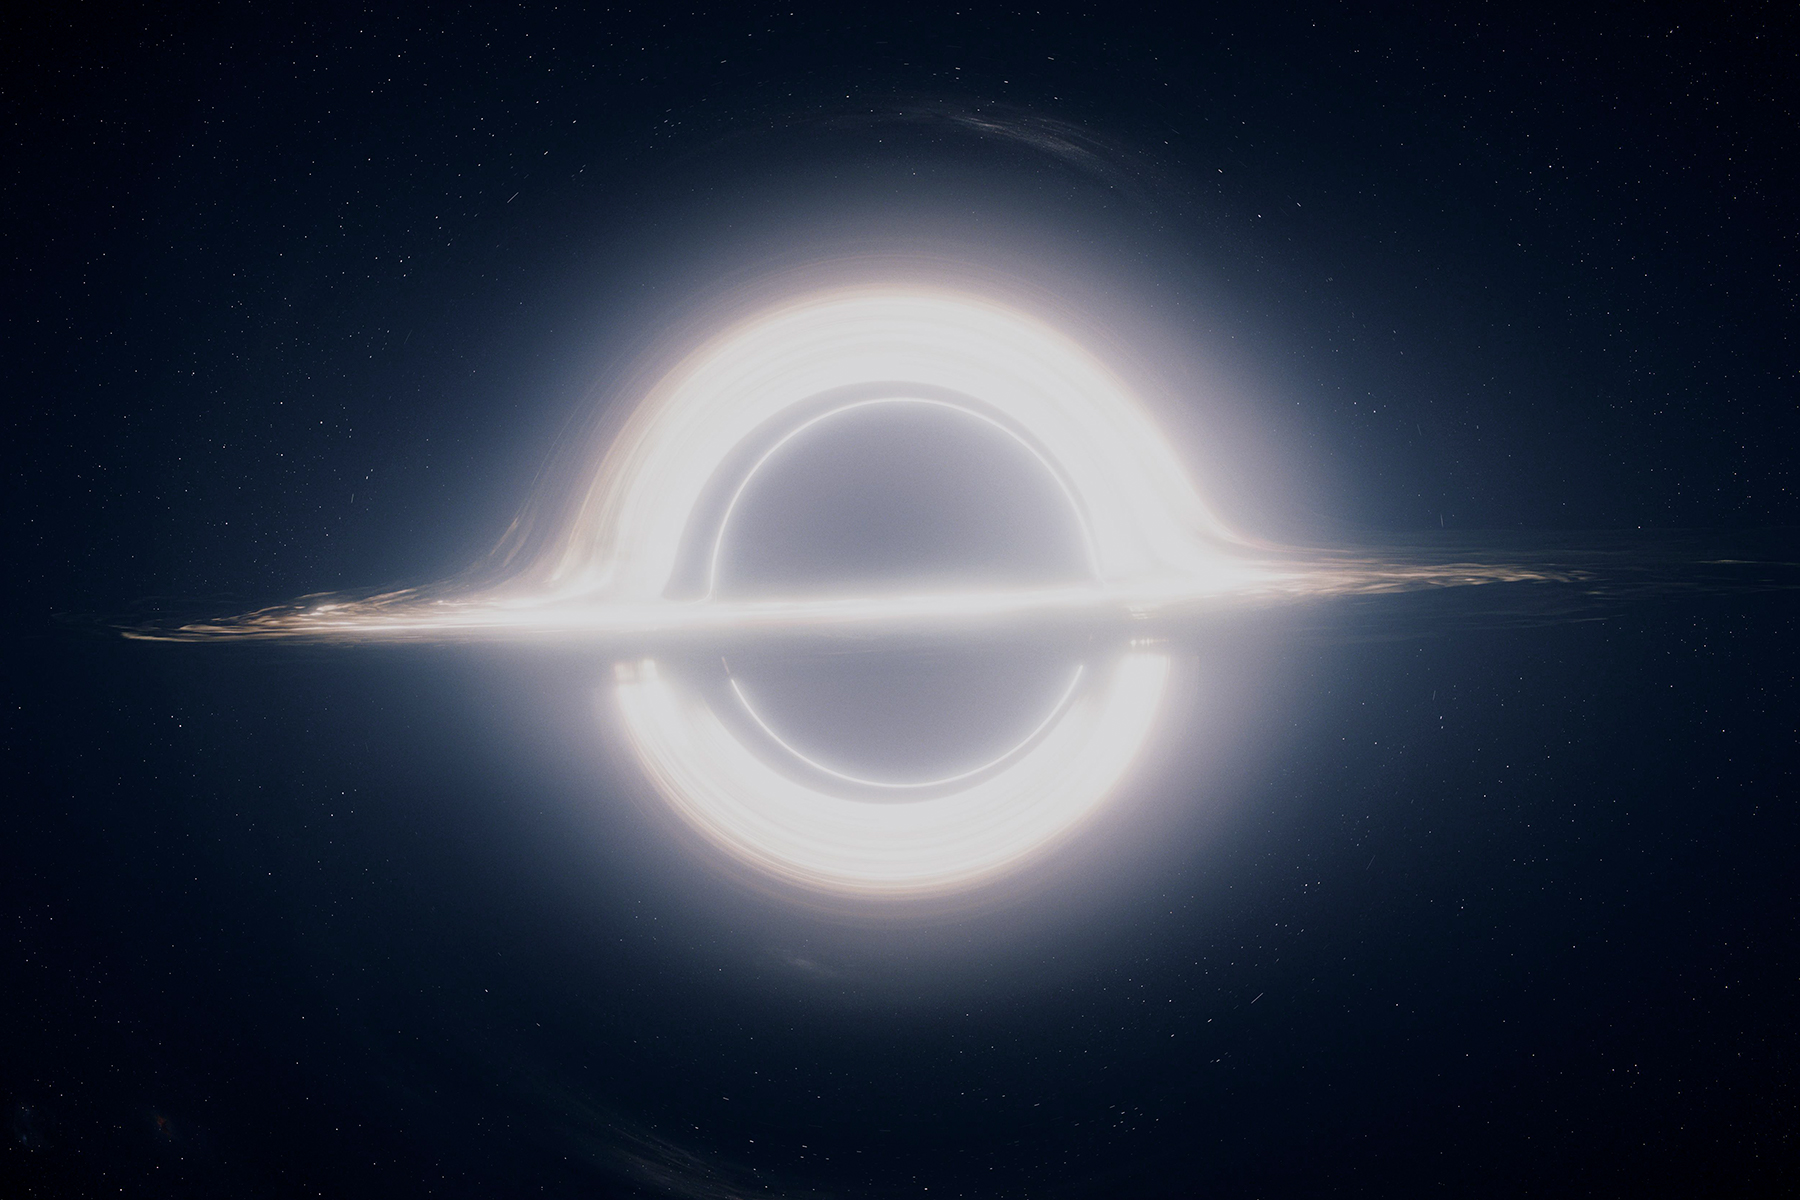
\includegraphics[width=.7\textwidth]{fig/chpt01/blackhole.jpg}
    \caption{\small 电影 \textit{Interstellar} 中黑洞 Gargantua 设定为一颗古老的巨型旋转黑洞,周围绕有的星尘称为\textbf{吸积盘}(accretion disk)。受引力作用,其间有高温物化反应,大量射线放出,包括可见光。观众看来,视界遮挡了部分光源,但光线仍可绕过视界,故视觉上吸积盘仿佛包裹了视界。}
\end{figure}
Wheeler 将视界半径超过其自身半径的星体称为\textbf{黑洞}(black hole)。目前已观测到这种星体。视界所包围的时空区域称为\textbf{黑洞区域},视界又可称黑洞表面。若星体斥力不能与引力抗衡,则质量将无限坍缩至 $r=0$,因而视界内极为空旷。

考虑到球对称性,只需研究 2 维 $\d s^2=-\left(1-{2M}/{r}\right)\,\text d t^2+\left(1-{2M}/{r}\right)^{-1}\text d r^2$。
用\textbf{类光测地线族}(family of null geodesics)研究时空的因果结构。
2 维图上每一点都可确定两条不同的类光测地线,所有类光测地线可分为两类。空间上朝外的称\textbf{外向}(outgoing),反之称\textbf{内向}(incoming)。
令 $\d s^2=0$,则
\eq{\label{dia_Sch}
t=\pm\left(r+2M\ln|r-2M|\right)+C.
}
考虑 $r>2M$,上式正负号取正后斜率为正,为外向族,负号对应内向族。然而 $r=2M$ 时 $t\to\infty$,故在 $\{t,x\}$ 系下任何物质永不落入视界。但请注意,同时的相对性导致“永远”的相对性。
考虑静止于 $r=r_0$ 的钟,其固有时满足 $\dv*{\tau}{t}={\sqrt{1-2M/r_0}}$。当 $r_0\to 2M$ 时 $\dv*{\tau}{t}\to 0$,说明在 Schwarzschild 系下,钟在视界处的读数 $\tau$ 近乎定格。
物理意义是,遥远观者需要通过对钟建立正交性,然而反射事件越接近视界,光就越难逃离,遥远观者接受光信号的用时就越来越久,对钟过程极为缓慢,从而出现永不落入的现象。
欲连续地描述粒子落入视界的过程,就是找到坐标系使测地线连续,也即消除度规的奇性。

考虑从 $r=r_0$ 释放的自由落体质点 $Z^\mu$。E-L 方程给出 $\dv{\tau}(g_{\mu\nu} Z^\nu)=\frac 12 g_{\alpha\beta,\mu} Z^\alpha Z^\beta$。由 $g_{\mu\nu,0}=0$ 知 $g_{0\nu} Z^\nu=\text{常数}$。取 $\nu=0$ 有 $Z^0=E/(1-{2M}/{r})$,其中 $E=1-2M/r_0$,因为 $r=r_0$ 时 $Z^0=1$。由模长归一性,并取内向有 $Z^1=-\sqrt{E^2-1+{2M}/{r}}$。对偶为 $Z_0=-1,Z_1=-(1-{2M}/{r})^{-1}{\sqrt{2M/r}}$。
下面按自由落体者建立新系 $\{\tau,R\}$。$\tau$ 可称\textbf{自由落体时}。由 $\tilde Z^\mu=\delta^\mu_0$ 知 $\tilde g_{0 0}=\tilde g_{\mu\nu}\tilde Z^\mu\tilde Z^\nu=-1$ 且对偶为 $\tilde Z_\mu = \tilde g_{\mu0}$。设 $\tilde g_{01} = 0$ 表示已对钟,则 $\tilde Z_0 = -1,\tilde Z_1 = 0$。代入 $\pdv{\tilde x^\mu}{x^\nu}\tilde Z_\mu=Z_\nu$ 得 $\pdv{\tau}{t}=-Z_0,\pdv{\tau}{r}=-Z_1$,即
\eq{
    \d\tau=\d t+\frac{\sqrt{2M/r}}{1-{2M}/{r}}\d r\implies \tau = t+2 \sqrt{2Mr}+2M\ln\abs{\frac{\sqrt{r}-\sqrt{2M}}{\sqrt{r}+\sqrt{2M}}}.
}
其中积分常数均取零。做 $t\to\tau$ 变换后有
\eq{\d s^2=-\left(1-\frac{2M}{r}\right)\d\tau^2+2\sqrt{\frac{2M}{r}}\d\tau\,\d r+\d r^2=-\d\tau^2+\left(\sqrt{\frac{2M}{r}}\d\tau+\d r\right)^2,}
这称为\textbf{Gullstrand–Painlevé 系},可以再加上没动过的 $r^2\d\Omega^2$。
分量收敛且 $g\ne 0$ 表明已消除了视界奇性,但还不满足 $\tilde g_{00}=-1,\tilde g_{01}=0$。
继续变换。
记 $\d R=A\d t+B\d r$,代入 $\tilde Z^1=\pdv{R}{x^\nu}Z^\nu$ 可知 $B=-A Z^0/Z^1$,则
$\d R=A\Big(\d t+\frac{\sqrt{r/2M}}{1-{2M}/{r}}\d r\Big)=A (\d\tau+\sqrt{r/2M}\d r)$,直接代入上述度规可知 $g_{11}=\frac{2M}{A^2r}$。
可见 $R$ 可确定到只差缩放函数 $A(t,r)$,因为各落体者间距任意。
不妨取 $A=1$,则 $R=\tau+\frac 23(2M)^{-1/2}r^{3/2}$。度规表为
\eq{
    \d s^2=-\d\tau^2+\frac{2M}{r}\d R^2+r^2\d\Omega^2,\quad r=(2M)^{1/3}\left(\frac 32(R-\tau)\right)^{2/3}.
}
这称为\textbf{Lemaître 系}。这是非稳态系,直观上,沿着落体运动 $R=R_0$ 当然感受到变化的引力场。
自由落体者在 $\tau=R$ 到达 $r=0$。这说明视界内时空极为空旷,且一旦进入视界便无法逃脱,最终落入奇点。

可见,显然


 则自然就

计算可得如下的\textbf{Kretschmann 标量}
\eq{
R_{\mu\nu\sigma\lambda}R^{\mu\nu\sigma\lambda} = \frac{48 M^2}{r^6},
}
上式在 $r=0$ 发散。这问题其实很严重,因为我们只是框定一堆物质,便使得光滑的时空上戳出一个“洞”,令人难以接受。$r=0,2M$ 两处的奇性在此体现出区别:上式在 $r=2M$ 有意义。
既然曲率在 $r=2M$ 处并不奇异,那就有可能找到坐标系使度规分量不发散。这种奇性称为\textbf{坐标奇性}或\textbf{假奇性},可尝试消除。
$r=0$ 的奇性就称\textbf{时空奇性}或\textbf{真奇性},因为曲率发散与坐标系无关。此点称\textbf{奇点}\footnote{英文亦是 singularity。为表述性质和地点两种概念,中文语境里可区分使用。但注意奇点不一定仅位于空间点。}。



并且,当视界内部很空旷时,对探险者而言,其进入视界时并无触觉,若稍有不慎,未能警觉自己所处位置,则很可能多走一步而遁入厄运。

当然,探险者还是能通过视觉上“眼前一黑”来观察,但更可怕的是,探险者并非真正的质点,而不同位置所受引力在此极端地带将差距巨大,因此潮汐力(对应于曲率大小)极有可能撕碎探险者,除非视界半径很大而稀释了曲率。此外,前文用测量效应说明了静态观者对探险者的观察,亦可用视觉效应这种现象。若静态观者借光信号观察探险者,则从图容易看出,随探险者逐渐接近视界,探险者所发出的光将越来越晚地到达静态观者,而坠入的画面无法传播出来。


\section{修改引力理论}
\subsection{宇宙学}
观测结果建议,宇宙在大尺度上\textbf{均匀}(homogeneous)且\textbf{各向同性}(isotropic)。这使得不能用非零质量密度和常数场强求解 Poisson 方程,因为在无限充斥的物质场中,试图计算某点场强时要涉及全空间体积分,而这种积分是反常的,其结果结果取决于有限域趋于无穷的方式。方式不同可得到“为零”或“发散”的结果。因此 Newton 引力论很难发展出宇宙学。

但广义相对论允许我们研究均匀各向同性的解及其扰动。
宇宙学的早期发展毫无疑问是 Einstein 带头。当时占统治地位的观点是静态宇宙。这使得 Einstein 为强行凑出静态解而修改场方程。注意除了选择 $R$,还可注意 $\sqrt{-g}\d[4]{x}$ 本身就已广义不变,故可考虑 $\mathcal L=\frac{1}{2\kappa}\left(R-2\Lambda\right)+\mathcal L_M$,结果是
\eq{
    R_{\mu\nu}-\frac12 g_{\mu\nu} R + \Lambda g_{\mu\nu}=\kappa T_{\mu\nu},
}
其中 $\Lambda$ 称为\textbf{宇宙学常数}(cosmological constant)。
根据具体的宇宙模型以及观测结果,可以确定其数值。
当然,在假设静态的情况下也能强行计算其值。但现代观点自 Hubble 开始普遍认为宇宙是\textbf{膨胀的}(expanding)。比如,\textbf{FLRW 解}就是膨胀宇宙的一阶近似。在膨胀模型下可不引入 $\Lambda$,故 Einstein 认为添加 $\Lambda$ 是其\textit{一生中所犯的最大错误}。1967 年 Hawking 证明了膨胀宇宙在时间上回溯可到达奇点,这被称为\textbf{宇宙大爆炸}(the big bang)。1990 年代的理论及观测显示,只有将 $\Lambda$ 重新写进来才能解释宇宙的\textbf{加速膨胀},其结果为 $\Lambda=1.1056\times 10^{-52}$\,m$^{-2}$。对通常的分析,这个数值太小,远不及 $\frac12 g_{\mu\nu} R$ 项的贡献,故会被忽略掉。
目前这一项被解释为\textbf{暗能量}(dark energy)的贡献。在量子场论中,能具备这一性质的概念只有真空能,然而两套理论给出的 $\Lambda$ 数值相差数量级很大。

还可考虑 $R_{\mu\nu} R^{\mu\nu},R_{\mu\nu\sigma\kappa}R^{\mu\nu\sigma\kappa}$ 等\textbf{Gauss-Bonnet 项}:
\eq{
    \mathcal L_G=\frac{1}{2\kappa}R+\alpha R_{\mu\nu} R^{\mu\nu}+\beta R^2+\gamma R_{\mu\nu\sigma\kappa}R^{\mu\nu\sigma\kappa}+\cdots,
}
甚至包括更高阶导数,其中耦合强度都是 $\hbar$ 量级的极小值。一般在日常尺度下可不考虑量子效应。

\subsection{Mach 原理及标量场}

Newton 为了解释绝对空间的存在性,提出了所谓的\textbf{水桶实验}。将一盛有清水的桶静置,并用一根长绳悬吊(图中略去)使桶可以靠绳索的扭力而转动;随后,尽可能使桶很快地加速旋转至某一角速度并保持。起初,桶相对于我们旋转,但(大部分)水由于惯性仍将保持静止,并且液面是平坦的;待桶的运动通过摩擦力传导至水,使水开始渐渐地随桶旋转,液面逐渐凹陷。在某个时刻,水和桶都将以该角速度旋转,即相对静止,液面凹陷呈抛物面状;尽可能很快地停止旋转,这个时候水由于惯性仍然要旋转一会儿才会静止,液面仍然凹陷。
虽说本质是思想实验,但其可行性还是挺大的:Newton 本人就声称“已经做过实验”,并对该结果表示肯定。
\begin{figure}[ht]\centering
    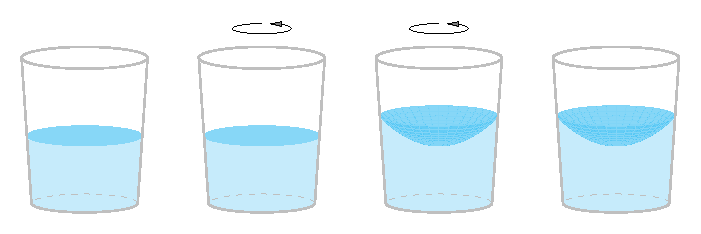
\includegraphics{fig/chpt01/spinning bucket.pdf}
    \caption{水桶实验}
\end{figure}
什么原因使液面凹陷?从经验中知道是水在相对于某个参考系旋转,进而产生了离心作用,但这个参考系是谁呢?起初水相对于环绕它的桶在旋转,随后水与桶一同旋转而相对静止的,但液面是凹陷的。因此,产生凹陷的旋转不是相对于水桶的旋转。Newton 认为这是相对于绝对空间的旋转。水面的凹陷是水的绝对运动的效果,通过凹陷程度可以测得其“绝对角速度”。Newton 认为如果水在其中旋转会凹陷,则这个参考系就是绝对空间。

19 世纪末,Mach 提出水并非相对于某种绝对介质旋转,而是相对于宇宙的全部物质组分,即星空背景。水凹陷是水的惯性效果,故 Mach 认为\textit{惯性需要在物质的相对运动中体现},或者\textit{物体惯性受到周围物质分布的影响}。这称为\textbf{Mach 原理},尽管是一条模糊的定性描述。准确地说,Mach 将桶参考系中所出现的惯性力理解为一种星空背景对水的作用,作用的强度体现为物体惯性,其大小与周围星空背景的质量及相对加速有关。比如,若周围物质很稀疏,就很难找到参照来判断一颗弹性球是否旋转,那么即使其旋转起来也不会形变。这似乎与引力很相似,但在实验上很难验证。因为反之需要加速周遭极大量的物质,绕着水桶旋转并观察水是否凹陷,尽管似乎直觉上应产生同样效果。

Einstein 也曾受到这一原理的启发,而去寻找惯性和引力的关系,最后抓住了等效原理。但实际上,等效原理给出的是新答案,即水是相对于局域惯性系运动。换言之,广义相对论已通过等效原理回答了这一问题。Einstein 起初以为广义相对论符合 Mach 原理,但现在看来显然不符合。且当代观点更多认为 Mach 原理至少在现有实验条件下是错误的。相反,等效原理受到支持的验证就多得多。若非要认为惯性起源于相互作用的话,由于局域惯性系是由外引力场决定的,因此可认为凹陷现象是水和引力场之间的互动造就的。目前用广义相对论回答“怎么办”是完全可行的,而“为什么”则是留给科学哲学。

1960 年代,Brans 和 Dicke\cite{Brans-Dicke} 提出了一个接近 Mach 原理愿景的引力理论。
首先注意,在地球的某个自由落体电梯中,等效原理的解释是电梯与乘客加速度一致,而 Mach 原理的解释是乘客的地球引力与星空背景的作用抵消。Newton 理论给出的地球引力为 $a=Gm/r^2$。假设星空背景有某种宇观质量 $M$ 和半径 $R$,并施加相同 $a$,根据量纲分析可知数量级上 $\frac{Gm}{r^2}\sim \frac{Rm}{Mr^2}$(几何制),因此 $\frac{1}{G}\sim\frac{M}{R}$。一种理解是 $\frac{M}{R}$ 由理论给出,而质量分布由广义相对论场方程的某个边界条件给出。还有一种是局部观察的 $G$(或场源质量)是随时空点变化的,其值由附近的质量分布决定。
假设 $G$ 是某个标量场的函数。首先想到 Ricci 标量,但它含有度规一阶导,随着与场源距离 $r$ 的增大,它比 $1/r$ 减小得还快。这种标量主要由附近质量分布决定,而非远处物质。因此,我们需要一个独立于度规以外的新标量场 $\phi$,但二者都用于描述引力场。假设理论是线性的,则前文表明乘客的惯性力贡献应是引力常数的倒数,即 $\phi\sim\frac{1}{G}$。
进而自由引力场加上标量场的部分为
\eq{
    \mathcal L_G=\frac{1}{16\pi} \left(\phi R-\frac{\omega(\phi)}{\phi}\partial_\mu \phi \partial^\mu \phi-2\Lambda(\phi)\right) ,
}
其中 $\omega$ 是耦合参数,$\frac{\omega}{\phi}$ 是为了使 $\omega$ 无量纲,并且还引入了$\Lambda(\phi)$ 代表可变的宇宙学常数。这就是\textbf{标量-张量理论}。准确地说,是
$\phi$ 的平均值 $\langle\phi\rangle$ 象征 $1/G$。

先对 $g^{\mu\nu}$ 变分,则
\begin{align*}
    16\pi \var(\mathcal L_G\sqrt{-g})&=\phi\left( G_{\mu\nu} \var g^{\mu\nu}+g^{\mu\nu}\var R_{\mu\nu}\right) \sqrt{-g}+ \Lambda g_{\mu\nu} \var g^{\mu\nu}\sqrt{-g}\\
&-\frac{\omega}{\phi}\left(\del_\mu\phi \del_\nu\phi-\frac 12 g_{\mu\nu}\partial_\lambda \phi \partial^\lambda\phi\right)\var g^{\mu\nu}\sqrt{-g},
\end{align*}
重点关注其中 $g^{\mu\nu}\var R_{\mu\nu}=2\nabla_\lambda(g^{\mu [\nu} \delta \Gamma_{\mu \nu}^{\lambda]})$。由于乘了 $\phi$,不能直接当做边界项丢掉,而要进一步用 $\var g^{\mu\nu}$ 表示克氏符变分。直接用协变导数 $\del_\mu g^{\sigma\lambda}+\Gamma^\sigma_{\mu\nu} g^{\nu\lambda}+\Gamma^\lambda_{\mu\nu} g^{\nu\sigma}=0$ 计算出克氏符。变分有 $\nabla_\mu \delta g^{\sigma\lambda}+g^{\nu\lambda}\delta \Gamma^\sigma_{\mu\nu} +g^{\nu\sigma}\delta \Gamma^\lambda_{\mu\nu} =0$。
用 $g^{\kappa\mu}$ 升指标,进行 $\kappa,\sigma,\lambda$ 轮换后加减消项,再缩并移项就有
\eq{
    \delta \Gamma_{\mu \nu}^\lambda=-\frac{1}{2}\left(g_{\kappa \mu} \nabla_\nu\delta g^{\kappa \lambda}+g_{\kappa \nu} \nabla_\mu\delta g^{\kappa \lambda}-g_{\mu \sigma} g_{\nu \kappa} \nabla^\lambda\delta g^{\sigma\kappa}\right).
}
进而与 $g^{\mu\nu}$ 缩并再取反称有
\eq{
    2g^{\mu [\nu} \delta \Gamma_{\mu \nu}^{\lambda]}=g_{\mu\nu}\nabla^\lambda \delta g^{\mu\nu} - \nabla_\mu\delta g^{\mu\lambda},
}
将该结果用于分部积分:
\begin{align*}
    2\int \phi \nabla_\lambda(g^{\mu [\nu} \delta \Gamma_{\mu \nu}^{\lambda]}) D^4x &\simeq -2\int  g^{\mu [\nu} \delta \Gamma_{\mu \nu}^{\lambda]} \nabla_\lambda \phi D^4x\\
    &= -\int  (g_{\mu\nu}\nabla^\lambda (\delta g^{\mu\nu})\nabla_\lambda \phi - \nabla_\mu(\delta g^{\mu\lambda}) \nabla_\lambda \phi)  D^4x\\
    &\simeq \int  (g_{\mu\nu} \delta g^{\mu\nu}\nabla^\lambda \nabla_\lambda \phi - \delta g^{\mu\lambda} \nabla_\mu\nabla_\lambda \phi)  D^4x\\
    &=\int  (g_{\mu\nu} \square_g \phi - \nabla_\mu\nabla_\nu \phi) \delta g^{\mu\nu} D^4x.
\end{align*}
故引入物质场后的结果为
\eq{
    \phi G_{\mu \nu}+\Lambda g_{\mu\nu}=8 \pi T_{\mu \nu}+\frac{\omega}{\phi}\left(\partial_\mu \phi \partial_\nu \phi-\frac{1}{2} g_{\mu \nu} \partial_\lambda \phi \partial^\lambda \phi\right)+\nabla_\mu \del_\nu \phi-g_{\mu \nu} \square_g \phi,
}
并注意其迹为
\eq{\label{eq:BDtrace}
    -R+4\frac{\Lambda}{\phi} =\frac{8 \pi}{\phi} T-\frac{\omega}{\phi^2}\partial_\lambda \phi \partial^\lambda \phi-\frac{3}{\phi}\square_g \phi.
}

再对 $\phi$ 变分:
\[16\pi\var(\mathcal L_G\sqrt{-g})= \left(\left(R-2\dv{\Lambda}{\phi}\right)\var\phi - \frac{1}{\phi}\del_\mu \phi \del^\mu \phi\dv{\omega}{\phi}\var\phi - \omega\var(\frac{1}{\phi}\del_\mu \phi \del^\mu \phi)\right) \sqrt{-g},\]
其中
\begin{align*}
    \int \var(\frac{1}{\phi}\del_\mu \phi \del^\mu \phi) D^4 x
    & =\int \left(-\frac{1}{\phi^2} \del_\mu \phi \del^\mu \phi \delta \phi+\frac{2}{\phi} \del^\mu \phi  \del_\mu \delta \phi\right) D^4 x \\
    & \simeq \int \left(-\frac{1}{\phi^2} \del_\mu \phi \del^\mu \phi \delta \phi-2 \nabla_\mu\left(\del^\mu \phi \frac{1}{\phi}\right) \delta \phi\right) D^4 x \\
    & =\int\left(-\frac{1}{\phi^2} \del_\mu \phi \del^\mu \phi \delta \phi-\frac{2}{\phi} \square_g \phi \delta \phi+\frac{2}{\phi^2} \del^\mu \phi \del_\mu \phi \var\phi\right) D^4 x\\
    & =\int\left(\frac{1}{\phi^2} \del_\mu \phi \del^\mu \phi  - \frac{2}{\phi} \square_g \phi \right)\delta \phi D^4 x.
\end{align*}
进而
\[
    R-2\dv{\Lambda}{\phi}-\frac{1}{\phi}\del_\mu \phi \del^\mu \phi\dv{\omega}{\phi}- \frac{\omega}{\phi^2} \del_\mu \phi \del^\mu \phi  + \frac{2\omega}{\phi} \square_g \phi=0.
\]
利用 \eqref{eq:BDtrace} 式替换掉 $R$ 可得
\eq{
    (3+2\omega) \square_g \phi+4\Lambda-2\phi\dv{\Lambda}{\phi}-\del_\mu \phi \del^\mu \phi\dv{\omega}{\phi}=8 \pi T.
}

具体地,考虑 $\dv*{\omega}{\phi}=0$ 和 $\Lambda=0$,则
\eq{
    \mathcal L_G=-\frac{1}{16\pi} \left(\phi R-\omega \phi^{-1} \partial_\mu \phi \partial^\mu \phi\right),
}
进而
\begin{gather}
    G_{\mu \nu}=\frac{8 \pi}{\phi} T_{\mu \nu}+\frac{\omega}{\phi^2}\left(\partial_\mu \phi \partial_\nu \phi-\frac{1}{2} g_{\mu \nu} \partial_\lambda \phi \partial^\lambda \phi\right)+\frac{1}{\phi}\left(\nabla_\mu \del_\nu \phi-g_{\mu \nu} \square_g \phi\right), \\
    \square_g\phi=\frac{8 \pi}{3+2 \omega} T.
\end{gather}
此即\textbf{Brans-Dicke 理论}。可见若 $\omega\to\infty$,则 $\phi$ 没有贡献,退回广义相对论。根据论文 \cite{Bhabra} 的结果,从 Schwarzschild 解的角度来看,对于非常大的 $\omega$,那么现有实验精度下,广义相对论和 Brans-Dicke 理论就已不可分辨。既然如此就选择广义相对论。截止到 2003年,飞往土星的 Cassini 飞船的 Doppler 跟踪(tracking)\cite{Will-thesis}的测量结果为 $\omega>40000$,即目前观测还是更倾向于广义相对论。

一个涉及宇宙暴胀的理论是 $f(R)$\textbf{理论},其中自由引力场的拉氏密度为 $\mathcal L_G=f(R)$。
记标量场 $f_R:=\dv*{f(R)}{R}$。变分有
\begin{align*}
\delta S_G &=  \int\left(f_R \delta R -\frac12 f(R) g_{\mu\nu}\delta g^{\mu\nu}\right) D^4x \\
&=  \int\bigg(f_R R_{\mu \nu} -\frac{1}{2} f(R) g_{\mu \nu} \bigg) \delta g^{\mu \nu}D^4x+2\int f_R \nabla_\lambda(g^{\mu [\nu} \delta \Gamma_{\mu \nu}^{\lambda]}) D^4x\\
&\simeq  \int\left(f_R R_{\mu \nu} -\frac{1}{2} f(R) g_{\mu \nu} +g_{\mu\nu} \square_g f_R - \nabla_\mu\nabla_\nu f_R\right) \delta g^{\mu\nu} D^4x,
\end{align*}
加上物质场的贡献有
\eq{
    f_R R_{\mu \nu}-\frac{1}{2} f(R) g_{\mu \nu}+g_{\mu \nu} \square_g f_R-\nabla_\mu \nabla_\nu f_R=\kappa T_{\mu\nu}.
}
可证 $f(R)$ 的作用实际上相当于引入额外标量场。我们以后再谈细节。

\subsection{Kaluza-Klein 理论}

我们甚至不排除更高维时空的存在,将四维时空中的相互作用视作更高维物理的结果。
Kaluza 最先注意到电磁张量看起来像截断克氏符:引入第五(空间)维度使得 $A_{\mu}=g_{\mu 4}$,假定 $g_{\mu\nu,4}=0$ 则
\eq{
    \Gamma^\mu_{\nu 4}=\frac{1}{2}g^{\mu\sigma}\left(2g_{4[\sigma,\nu]}+g_{\sigma\nu,4}\right)=-\frac{1}{2}F^\mu{}_{\nu}.
}
其中 $\mu,\nu$ 只取 $0,1,2,3$。假设五维“度规”形如
\eq{
    \d\hat s^2=\hat g_{ab}\d x^a\d x^b=g_{\mu\nu}\d x^\mu \d x^\nu+(\d x^4+\lambda A_\mu\d x^\mu)^2,
}
其中 $a,b$ 取 $0,1,2,3,4$。
也即
$\hat g_{\mu\nu}=g_{\mu\nu}+\lambda^2 A_{\mu}A_{\nu},\ \hat g_{\mu 4}=\lambda A_\mu,\ \hat g_{44}=1$。
这一“度规”显然对任意四维变换 $x'^\mu(x^\nu)$ 或平移 $x'^5=x^5+f(x^\nu)$ 不变,但对任意五维变换可变,故并非真正的五维流形上的度规。后者的结果正是规范变换 $A'_\mu=A_\mu-\del_\mu f$。
换言之,我们将 U(1) 对称性的内部自由度 $\theta$ 解释到了第五维 $x^4$。
依次计算克氏符、Ricci 张量和 Ricci 标量可得
\eq{
    \hat R=R-\frac{\lambda^2}{4}F_{\mu\nu}F^{\mu\nu}.
}
这意味着五维几何 $\hat{\mathcal L}=\hat R$ 可在四维时空下分化出引力和电磁作用,称为\textbf{Kaluza 奇迹}。为求五维度规行列式,只需先对角化。考虑
$H^\mu{}_{\nu}=\delta^\mu_\nu,\ H^4{}_{\nu}=-\lambda A_\nu,\ H^\mu{}_{4}=0,\ H^4{}_{4}=1$,
则 $\hat g_{\mu a} H^a{}_{\nu}=g_{\mu\nu},\ \hat g_{\mu a} H^a{}_{4}=\lambda A_\mu,\ \hat g_{4 a} H^a{}_{\nu}=0,\ \hat g_{4 a} H^a{}_{4}=1$。因此 $\hat g=g$。
但我们需要使对 $x^4$ 的积分收敛。注意 U(1) 变换中 $\theta$ 是周期等效的,因而第五维度对应于某个圆周。因而 U(1) 等效为了 SO(2)。这便是\textbf{紧化}(compactication)思想之源,最先由 Oskar Klein 引进。$g_{\mu\nu,4}=0$ 也称\textbf{圆柱条件}(cylindricity condition)。五维“时空”并非流形,在数学上是\textbf{纤维丛}(fiber bundle),四维时空作为其\textbf{底流形}而第五维圆圈作为其\textbf{纤维}。假设半径 $L$,则
\eq{
    \hat S=\frac{1}{16\pi\hat G}\int \hat R \sqrt{-\hat g} \d^5 x=\frac{L}{8\hat G}\int\hat R \sqrt{- g} \d^4 x,
}
Gauss 几何制下取 $\hat G=2\pi L,\lambda=2$ 即得真空 Einstein-Maxwell 作用量。再考虑五维测地线方程 $\ddot x^a+\Gamma^a_{bc}\dot x^b \dot x^c=0$。首先由圆柱条件知守恒量 $\pdv*{\mathcal L}{\dot x^4}\propto\dot x^4+A_\mu\dot x^\mu$。剩余分量为
\eq{
    \ddot x^\lambda+\Gamma^\mu_{bc}\dot x^b \dot x^c=\ddot x^\lambda+\Gamma^\lambda_{\mu\nu}\dot x^\mu \dot x^\nu-F^\lambda{}_\mu\dot x^\mu(\dot x^4+A_\nu\dot x^\nu)=0,
}
若用荷质比来确定守恒量,则这正是 Lorentz 力定律 $\dot x^4+A_\nu\dot x^\nu=q/m$。从而经典电磁力、经典引力得到统一。
带电粒子与中性粒子具有不同运动,这并不违反等效原理,而只是因为它们在 $x^4$ 上有不同初速度。

这一理论当然差强人意。$\hat R_{ab}=0$ 的真正结果为
\eq{
    F_{\mu\nu}F^{\mu\nu}=0,\quad \nabla_\mu F^{\mu\nu}=0,\quad R_{\mu\nu}=2 F_{\mu\sigma}F_{\nu}{}^{\sigma},
}
第三式只是真空 Einstein-Maxwell 方程 $R_{\mu\nu}=8\pi T_{\mu\nu}$ 在第一式成立的特例。第一式源于 $\hat R_{44}=0$。这是因为变分原理并不能保证 $\hat g_{44}=1$ 假设。从而,五维假设显得非常人为。最重要的是,我们始终在讨论经典理论,并未真正考虑量子力学。实际上,强、弱相互作用的概念在 Einstein 逝世后才被彻底确立。

此外还必须解释为何从未发现第五维度。置五维闵氏时空上的复标量场 $\hat\phi$。方便起见考虑无质量,Klein-Gordon 方程为
\eq{
    \hat\eta^{ab}\del_a\del_b\hat\phi=0,\quad \hat\phi=\sum_n\phi_n(x^\mu)\e^{\i n x^4/L},
}
其中由周期性 $x^4\sim x^4+2\pi L$,可对 $\hat\phi$ 作 Fourier 展开使其与 $x^4$ 的依赖关系更明确。代入展开式得到无穷多个解耦方程,即对 $\hat\phi$ 的无穷多 Fourier 模 $\phi_n$ 均有
\eq{
    (\square-m_n^2)\phi_n^2=0,\quad m_n^2={n^2}/{L^2}.
}
其中质量项源于 $\del_{44}$。可见五维时空上的无质量标量场会产生 $n=0$ 的四维无质量场\footnote{但仍有 d'Alembert 方程,故内部空间是谐振的或振动模固定。}、$n\ne 0$ 的无穷多有质量场。这种质量称为 Kaluza-Klein 模。

四维闵氏度规在五维上的拓展其实应为 $\d\hat s^2=\eta_{\mu\nu}\d x^\mu \d x^\nu+(\d x^4+\lambda A_\mu\d x^\mu)^2$,则 $\hat g=g=-1$。因此 $\hat g^{\mu\nu}=\eta^{\mu\nu},\hat g^{\mu 4}=-\lambda A^\mu,\hat g^{44}=1+\lambda^2 A^\mu A_\mu$。
Klein-Gordon 方程变为
\[
    0=\square_{\hat g}\hat\phi=\del_a\left(\hat g^{ab}\del_b \hat\phi\right)=\eta^{\mu\nu}(\del_\mu-\lambda A_\mu\del_4)(\del_\nu-\lambda A_\nu\del_4)\hat\phi+\del_4^2\hat\phi,
\]
将 Fourier 分解代入,则对任意 $\phi_n$ 有
\[
    \left(\eta^{\mu\nu}\left(\del_\mu-\i\frac{\lambda_n}{L} A_\mu\right)\left(\del_\nu-\i\frac{\lambda_n}{L} A_\nu\right)-m_n^2\right)\phi_n=0,
\]
可见非零模不仅有质量,且在规范场 $A_\mu$ 下带电。$\del_\mu-\lambda m_n A_\mu$ 与规范协变导数 $\del_\mu-\i ne A_\mu$ 对比得元电荷 $e=\lambda/L$。还原国际单位有 $e=\hbar\lambda/L$,以及 $\frac{c^4}{16\pi G}R-\frac{1}{4\mu_0}$。

$\nabla^\mu\phi\nabla_\mu\phi$ 代替即可,因而算子 $\square$ 换为 $\square_g$。

时空各点的额外维蜷缩(curled up),从而只剩下我们经验中看到的时空本身。

尽管有诸多缺陷,Wheeler 仍表示“几何动力学”拓展到其它相互作用是有希望的。20 世纪末,\textbf{弦论}(string theory)继承了高维几何的衣钵,利用极小对象“弦”部分地得到了广义相对论、量子场论的结果。此外还有企图构建背景无关量子场论的\textbf{圈量子引力}(loop quantum gravity)、研究非交换几何的\textbf{CLCB 理论},它们皆只部分地回答了量子引力的疑难。目前前沿话题还包括引力同统计物理、信息论的联系,诸如\textbf{熵力理论}、\textbf{黑洞信息学},以及受场论和凝聚态影响的\textbf{超对称理论}。
我们以后再详细学习。

引力是目前已知相互作用中最弱的。两个质子之间的静电斥力比它们之间的引力大 $1.2 \times 10^{36}$ 倍。这意味着即使各种量子引力理论层出不穷,但以当代技术,仍然很难直接做实验以获取有效数据。目前多用宇宙学观测所得到早期宇宙的数据来筛选理论。“大一统理论”通常指沿标准模型的思路,将强相互作用同电弱作用统一的尝试。狭义上的量子引力理论只涉足引力量子化问题,广义的量子引力理论或许是人们所希望的“万物理论”。

\section{标架表述}

还可考虑有挠时空,$g_{\mu\nu},T^\lambda{}_{\mu\nu}$ 一齐作为引力场的基本物理量。这种理论发展为\textbf{引力规范理论},典型地如\textbf{Einstein-Cartan 理论}。这些理论多采用了更为数学、但实质等价于 $g_{\mu\nu},T^\lambda{}_{\mu\nu}$ 形式的语言,故暂时只扼要介绍。其中 2 阶情形的最一般的规范理论作用量为
\eq{
\begin{aligned}
\mathcal L_G= & -\frac{1}{2\kappa}(R-2 \Lambda)+a_1 R_{\alpha \beta \mu \nu} R^{\alpha \beta \mu \nu}+a_2 R_{\alpha \beta \mu \nu} R^{\mu \nu \alpha \beta} \\
& +a_3 R_{\alpha \beta \mu \nu} R^{\alpha \mu \beta \nu}+b_1 R_{\alpha \beta} R^{\alpha \beta}+b_2 R_{\alpha \beta} R^{\beta \alpha} \\
& +c_1 T_{\alpha \beta \gamma} T^{\alpha \beta \gamma}+c_2 T_{\alpha \beta \gamma} T^{\beta \gamma \alpha}+c_3 T^\beta{}_{\alpha \beta} T_\gamma{}^{\gamma \alpha}.
\end{aligned}
}
其中 $R_{\alpha \beta \mu \nu}$ 是一般的\textbf{有挠 Riemann 曲率},前一对指标与后一对指标没有对称性,前一对指标也没有反称性。但 Ricci 张量仍按 $R_{\alpha \beta}=R^\mu{ }_{\alpha \mu \beta}$ 定义。其中的指标升降均在 $g_{\mu\nu}$ 下。

\section{哈氏理论}
\subsection{3+1 分解}

\subsection{初值问题}

\section{场论 Noether 定理}\label{sec:Noether}

